%%%%%%%%%%%%%%%%%%%%%%%%%%%%%%%%%%%%%%%%%%%%%%%%%%%%%%%%%%%%%%%%%%%%%%%%%%%%%%%
%%%%%%%%%%%%%%%%%%%        MANUAL VISUAL STUDIO         %%%%%%%%%%%%%%%%%%%%%%%
%%%%%%%%%%%%%%%%%%%%%%%%%%%%%%%%%%%%%%%%%%%%%%%%%%%%%%%%%%%%%%%%%%%%%%%%%%%%%%%
% !TeX program = lualatex
\documentclass[a4paper,11pt,twoside,english]{book}
%\documentclass[a4paper,twoside,english]{book}




\usepackage[
paperwidth=16.99cm,
paperheight=24.40cm,
left=2.4cm,
right=2cm,
top=2.95cm,
bottom=2.2cm,
twoside
]{geometry}


\usepackage[width=16.99truecm,height=24.40truecm,center]{crop}
%\usepackage[frame,width=16.99truecm,height=24.40truecm,center]{crop}
%\usepackage[a4,frame,center]{crop}


\usepackage{epic}
\usepackage[english]{babel} % English language/hyphenation


%___________________ FONTS ______________________________________________
\usepackage{amsfonts}
\usepackage{amssymb}
\usepackage{amsmath}
%\usepackage{txfonts}
\usepackage{mathrsfs}
\usepackage{mathdots}
\usepackage{lmodern}
%\usepackage[classicReIm]{kpfonts}
\usepackage{physics}    %  partial and total derivatives  

 \usepackage[utf8]{inputenc}
%___________ MATH THEOREMS
\usepackage{amsthm}
\usepackage{cancel}
\usepackage{mathtools}
\usepackage{mleftright}




% __________________________FANCY CHAPTERS _____________________________ 
%Options: Sonny, Lenny, Glenn, Conny, Rejne, Bjarne, Bjornstrup
%\usepackage[Sonny]{fncychap}
%\usepackage[Glenn]{fncychap} %1
%\usepackage[Conny]{fncychap}
%\usepackage[Rejne]{fncychap}
%\usepackage[Bjarne]{fncychap} %1
%\usepackage[Bjornstrup]{fncychap}
\usepackage[Lenny]{fncychap}

%_______________________ GLOSSARIES & NOMENCLATURE

%\usepackage{nomencl}

%\usepackage{glossaries}

%__________________________HEADERS & FOOTERS_____________________________
\usepackage{fancyhdr}


\pagestyle{fancy} % Enables the custom headers/footers
\lhead{\thepage}
\chead[]{}
\fancyhead[R]{\leftmark}

%To make the head rule
\usepackage{etoolbox}
\makeatletter
\patchcmd{\headrule}{\hrule}{\color{mygray}\hrule}{}{}
\makeatother


\renewcommand{\headrulewidth}{0.5pt} % No header rule
\renewcommand{\footrulewidth}{0.5pt} % Thin footer rule


%%PARA DOS CARAS
%\fancyhf{}             %allows additional selectors H (header) and F (footer)
\fancyhead[RO]{ \thepage}
\fancyhead[LE]{ \thepage}
%\fancyhead[LE,RO]{...}
\fancyhead[RE]{\sffamily\scshape\footnotesize\leftmark}
\fancyhead[LO]{\sffamily\scshape\footnotesize\rightmark}
\fancyfoot[CE,CO]{}
\fancyfoot[LE,RO]{}











%\usepackage{footmisc} %[norule]

%
%\renewcommand{\headrulewidth}{0.5pt} % No header rule
%\renewcommand{\footrulewidth}{0.5pt} % Thin footer rule
%
%\fancyhead[RO]{ \thepage}
%\fancyhead[LE]{ \thepage}
%%\fancyhead[LE,RO]{...}
%\fancyhead[RE]{\sffamily\scshape\footnotesize\leftmark}
%\fancyhead[LO]{\sffamily\scshape\footnotesize\rightmark}
%\fancyfoot[CE,CO]{}
%\fancyfoot[LE,RO]{}




%%PARA DOS CARAS
%\fancyhf{}             %allows additional selectors H (header) and F (footer)
%\pagestyle{fancy}
%\fancyhead[RO]{ \thepage}
%\fancyhead[LE]{ \thepage}
%%\fancyhead[LE,RO]{...}
%\fancyhead[RE]{\sffamily\scshape\footnotesize\leftmark}
%\fancyhead[LO]{\sffamily\scshape\footnotesize\rightmark}
%\fancyfoot[CE,CO]{}
%\fancyfoot[LE,RO]{}





%Allow us to make the rules larger
%
%\renewcommand{\headrulewidth}{0.5pt} % No header rule
%\renewcommand{\footrulewidth}{0.5pt} % Thin footer rule
% Headers - all currently empty
%\lhead{ }
%\chead{}
%\rhead{}
%% Footers
%\lfoot{}
%\cfoot{}
%%\rfoot{\footnotesize Page \thepage\ of \pageref{LastPage}} % "Page 1 of 2"
%\rfoot{\footnotesize \thepage\ }

%\usepackage{lettrine} % Package to accentuate the first letter of the text


%
%\renewcommand{\headrulewidth}{0.5pt} % No header rule
%\renewcommand{\footrulewidth}{0.5pt} % Thin footer rule
%
%
%%\renewcommand{\headrulewidth}{0.5pt} % No header rule
%%\renewcommand{\footrulewidth}{0.5pt} % Thin footer rule
%
%%%PARA DOS CARAS
%%\fancyhf{}                %allows additional selectors H (header) and F (footer)
%\fancyhead[RO]{ \thepage}
%\fancyhead[LE]{ \thepage}
%%\fancyhead[LE,RO]{...}
%\fancyhead[RE]{\sffamily\scshape\footnotesize\leftmark}
%\fancyhead[LO]{\sffamily\scshape\footnotesize\rightmark}
%\fancyfoot[CE,CO]{}
%\fancyfoot[LE,RO]{}
















%_________________ GRAPHS ______________________________________________
\usepackage{float} % Force image position
\usepackage{color}
\usepackage[dvipsnames]{xcolor}
\usepackage[font=small]{caption}
\usepackage{graphicx} % For pictures
\usepackage{epstopdf}
\usepackage{placeins}
\usepackage{tikz}
\usetikzlibrary{arrows,arrows.meta,positioning,shapes.geometric,shapes}
\usetikzlibrary{decorations.markings}

\usetikzlibrary{matrix}
\usepackage{pgfplots}
\usepackage{pgfplotstable}
\usepackage{pgf}
\usepackage{pgfcalendar}
%\usepackage{gnuplottex}
\usepgfplotslibrary{dateplot,statistics}
\usepgfplotslibrary{patchplots}
\usepgfplotslibrary{colormaps}
\usetikzlibrary{colorbrewer}
\usepgfplotslibrary{colorbrewer}
\usetikzlibrary{calc,intersections} 
\pgfplotsset{compat=1.12}
\usepackage{xifthen}
\usepackage{shellesc}
%\usetikzlibrary{external}
%\tikzexternalize[prefix=figures/]
%, shell escape=-enable-write18, shell escape=-enable-write18
%________________________ TABLES________________________________________
\usepackage{booktabs} % Horizontal rules in tables


%_____________________ TABLE OF CONTENTS _______________________________
\usepackage{makeidx} %Table of contents
%\PassOptionsToPackage{hyphens}{url}\usepackage{hyperref}
\PassOptionsToPackage{hyphens}{url}\usepackage[driverfallback=dvipdfmdvipdfm,colorlinks=true,linkcolor=black,breaklinks=true]{hyperref}  % Para incluir hipervinculos en el pdf
\hypersetup{citecolor=blue, urlcolor=blue}%,hyperfootnotes=false}       %Blue is different from blue, Blue is darker


\usepackage{enumitem} % Edit the itemizes
%\usepackage{titletoc,tocloft} % this two lines quit the indent that latex make between
% To change the format to the subsections
\usepackage{titlesec}
\usepackage{todonotes}


% ______________________EXTRA SPACE IN TABLES ______________________________
\usepackage{setspace}

 %_____________________________________ It is used to determine the number of pages in the document ____________________________(for "Page X of Total")
\usepackage{lastpage}



%\usepackage{extsizes} %14pt font size is not in the normal sizes of latex, we need this package


%_________________________The easylist package for numbered items____________________________________
%\usepackage[ampersand]{easylist}
\usepackage{subcaption}



%___________________ It enhances cross-reference ________________________________________
%\usepackage{cleveref}
%\usepackage{nameref}

%__________LUALATEX

%\usepackage{luatex85}



\usepackage{titling} % Allows custom title configuration
%\usepackage[a4,frame,center]{crop}






%\graphicspath{ {images/} }
%\newcommand{\folder}{./libraries}


\definecolor{DarkGoldenrod}{rgb}{0.8,0.6,0.1}
\definecolor{DarkRed}{rgb}{0.5,0.1,0.1}
\definecolor{DarkRedPart}{rgb}{0.3,0.1,0.2}

% Defines the gold horizontal rule around the title
%\newcommand{\HorRule}{\color{DarkGoldenrod} \rule{\linewidth}{1pt}}




\usepackage{titling} % Allows custom title configuration
% Defines the gold horizontal rule around the title
\newcommand{\HorRule}{\color{DarkGoldenrod} \rule{\linewidth}{1pt}}

\newcommand{\vect}[1]{\boldsymbol{#1}}




\definecolor{mygray}{gray}{0.8}
\definecolor{mygray2}{gray}{0.4}
\definecolor{mygreen}{rgb}{0.0, 0.42, 0.24}
\definecolor{myred}{rgb}{0.8, 0.0, 0.0}
\definecolor{myorange}{rgb}{0.91, 0.41, 0.17}
\definecolor{myblue}{rgb}{0.0, 0.44, 1.0}







%To make the head rule
\usepackage{etoolbox}
\makeatletter
\patchcmd{\headrule}{\hrule}{\color{mygray}\hrule}{}{}
\makeatother




%\setlength{\cftsecindent}{-0.8cm} % the section and the subsection in the table of contents
%\setlength{\cftsubsecindent}{-0.6cm} % the section and the subsection in the table of contents


% Replace the title of the table of contents 
\addto\captionsenglish{
    \renewcommand{\contentsname}%
    {}% Here it goes the new title
}

% Here we give the color to the subsections in the table of contents

%\makeatletter
%\let\stdl@subsection\l@subsection
%\renewcommand*{\l@subsection}[2]{%
%   \stdl@subsection{\textcolor{blue}{#1}}{\textcolor{black}{#2}}}
%\makeatother

% CHANGING THE FORMAT OF SUBSECTIONS AND SECTIONS

%\titleformat\subsection{}{}{0em}{ \bf \todo[inline, color=green!40]}[\vspace{0ex}]



%\titleformat\section{\centering \LARGE}{}{0em}{ \bf }[]

%\renewcommand{\thesubsection}{} %Subsection numbering
%\renewcommand{\thesection}{} %Section numbering



%\newcommand{\bluepageref}[1]{\textcolor{blue}{\pageref{#1}}}
\newcommand{\qnameref}[1]{``\nameref{#1}''}



% Comment the following to have chapters numbered without interruption (numbering through parts)
\makeatletter\@addtoreset{chapter}{part}\makeatother%

% \tableofcontents, without the title contents
%\makeatletter
%\@starttoc{toc}
%\makeatother
%



\newcommand{\remark}[1]{\textbf{``#1"}}





%\newcommand{\tit}{Raspberry Pi Server}
%\newcommand{\rhdr}{Developer Manual}


%\DeclareCaptionFormat{myformat}{#1#2#3\vspace{2ex}}
%\captionsetup{format=myformat}

%\captionsetup[lstlisting]{position=bottom,format=myformat}
%\usepackage{lstautodedent}

%commands

%\newcommand{\relpathto}[1]{./codes/#1}

%\renewcommand{\medskip}{\vspace{2ex}}

%\newcommand{\capof}[2]{\begingroup\captionof{#1}{#2}\endgroup}





%\usepackage{titling} % Allows custom title configuration
% Defines the gold horizontal rule around the title
%\newcommand{\HorRule}{\color{DarkGoldenrod} \rule{\linewidth}{1pt}}


%\graphicspath{ {images/} }



%\graphicspath{ {images/} }



% __________________________TEXT COLOR BOXES _____________________________ 
\usepackage{tcolorbox}      %Por alguna razón esto hay que declararlo después que scolor me parece, si no me salen muchos fallos. 
%\tcbuselibrary{listingsutf8} % o listings o minted, creo que para poner texto en latex y compilado al lado



%%%%%%%%%%%%%%%%%%%%%%%%%%%%%%%%%%%%%%%%%%%%%%%%%%%%%%%%%%%%%%%%%%%%%%%%%%%
%%                           TCOLORBOX BOXES                             %%
%%%%%%%%%%%%%%%%%%%%%%%%%%%%%%%%%%%%%%%%%%%%%%%%%%%%%%%%%%%%%%%%%%%%%%%%%%%
\newtcolorbox{IN}
{colback=blue!5!white,colframe=Blue!75!black,sharp corners=northwest, fonttitle=\bfseries, title=Important Notice}

\newtcolorbox{INWarning}
{colback=red!5!white,colframe=Red!75!black,sharp corners=northwest, fonttitle=\bfseries, title=Important Notice}

\newtcolorbox{mybox}[1]
{colback=blue!5!white,colframe=Blue!75!black,sharp corners=northwest, fonttitle=\bfseries, title=#1}

\newtcolorbox{ExampleCode}[1]
{colback=myred!5!white,colframe=myred!75!black,sharp corners=northeast, fonttitle=\bfseries, title=Example Code: #1}

\newtcolorbox{Example}[1]
{colback=myred!5!white,colframe=myred!75!black,sharp corners=northeast, fonttitle=\bfseries, title=Example: #1}


\usepackage[square,numbers]{natbib}




% ________________________CODE LENGUAGE________________________________________
\usepackage{listings}

\lstdefinelanguage{JavaScript}{
	keywords={typeof, new, true, false, catch, function, return, null, catch, switch, var, if, in, while, do, else, case, break, undefined},
	keywordstyle=\color{blue}\bfseries,
	ndkeywords={class, export, boolean, throw, implements, import, this},
	ndkeywordstyle=\color{darkgray}\bfseries,
	identifierstyle=\color{black},
	sensitive=false,
	comment=[l]{//},
	morecomment=[s]{/*}{*/},
	commentstyle=\color{red}\ttfamily,
	stringstyle=\color{orange}\ttfamily,
	morestring=[b]',
	morestring=[b]"
}



%\lstset{literate=%
%	{0}{{{\color{Green}0}}}1
%	{1}{{{\color{Green}1}}}1
%	{2}{{{\color{Green}2}}}1
%	{3}{{{\color{Green}3}}}1
%	{4}{{{\color{Green}4}}}1
%	{5}{{{\color{Green}5}}}1
%	{6}{{{\color{Green}6}}}1
%	{7}{{{\color{Green}7}}}1
%	{8}{{{\color{Green}8}}}1
%	{9}{{{\color{Green}9}}}1
%}


\newcommand{\lsthtml}{
	\lstset{
		language=html,
		basicstyle=\ttfamily\small,
		frame=single,
		showspaces=false,
		showstringspaces=false,
		backgroundcolor=\color{white},
		keywordstyle=\color{blue},
		deletekeywords={type},
		commentstyle=\color{mygreen},
		stringstyle=\color{violet},
		breaklines=true,
		alsoletter={.},morekeywords={nav,/nav}
	}
}
\newcommand{\lstbash}{
	\lstset{
		language=bash,
		basicstyle=\ttfamily\small,
		frame=single,
		showspaces=false,
		showstringspaces=false,
		backgroundcolor=\color{white},
		keywordstyle=\color{blue},
		deletekeywords={type},
		commentstyle=\color{mygreen},
		stringstyle=\color{violet},
		breaklines=true,
		alsoletter={.},
		morekeywords={ssh,scp,server.py,runserver.sh,killserver.sh,killemail.sh,runemail.sh}
	}
}
\newcommand{\lstpython}{
	\lstset{
		language=python,
		basicstyle=\ttfamily\small,
		frame=single,
		showspaces=false,
		showstringspaces=false,
		backgroundcolor=\color{white},
		keywordstyle=\color{blue},
		deletekeywords={type},
		commentstyle=\color{mygreen},
		stringstyle=\color{violet},
		breaklines=true,
		alsoletter={.,...},
		morekeywords={}
	}
}



\newcommand{\lstjs}{
	\lstset{
		language=JavaScript,
		extendedchars=true,
		basicstyle=\ttfamily\footnotesize,
		frame=single,
		showstringspaces=false,
		showspaces=false,
		numberstyle=\footnotesize,
		numbersep=9pt,
		tabsize=4,
		breaklines=true,
		showtabs=false,
		captionpos=b
	}
}




%
%
%\lstset{ %
%	backgroundcolor=\color{white},   % choose the background color; you must add \usepackage{color} or \usepackage{xcolor}
%	basicstyle=\footnotesize,%%        % the size of the fonts that are used for the code
%	breakatwhitespace=false,         % sets if automatic breaks should only happen at whitespace
%	breaklines=true,                 % sets automatic line breaking
%	captionpos=b,                    % sets the caption-position to bottom
%	commentstyle=\color{mygreen},    % comment style
%	deletekeywords={...},            % if you want to delete keywords from the given language
%	escapeinside={\%*}{*)},          % if you want to add LaTeX within your code
%	extendedchars=true,              % lets you use non-ASCII characters; for 8-bits encodings only, does not work with UTF-8
%	frame=single,                    % adds a frame around the code
%	keepspaces=true,                 % keeps spaces in text, useful for keeping indentation of code (possibly needs columns=flexible)
%	keywordstyle=\color{blue}\textbf,       % keyword style
%	language=Fortran,                 % the language of the code
%	otherkeywords={*,source},            % if you want to add more keywords to the
%	% set
%	numbers=none,                    % where to put the line-numbers; possible
%	% values are (none, left, right)
%	numbersep=5pt,                   % how far the line-numbers are from the code
%	numberstyle=\tiny\color{mygray}, % the style that is used for the line-numbers
%	rulecolor=\color{black},         % if not set, the frame-color may be changed on line-breaks within not-black text (e.g. comments (green here))
%	showspaces=false,                % show spaces everywhere adding particular underscores; it overrides 'showstringspaces'
%	showstringspaces=false,          % underline spaces within strings only
%	showtabs=false,                  % show tabs within strings adding particular underscores
%	stepnumber=2,                    % the step between two line-numbers. If it's 1, each line will be numbered
%	stringstyle=\color{mymauve},     % string literal style
%	tabsize=2,                       % sets default tabsize to 2 spaces
%	title=\lstname                   % show the filename of files included with \lstinputlisting; also try caption instead of title
%}
%
%
%


%\lstset{ %
%	backgroundcolor=\color{Goldenrod!10},   % choose the background color; you must add \usepackage{color} or \usepackage{xcolor}
%	basicstyle=\footnotesize\ttfamily,%%\small,               % the size of the fonts that are used for the code
%	breakatwhitespace=false,                % sets if automatic breaks should only happen at whitespace
%	breaklines=true,                 % sets automatic line breaking
%	captionpos=b,                    % sets the caption-position to bottom
%	commentstyle=\color{mygreen},    % comment style
%	deletekeywords={...},            % if you want to delete keywords from the given language
%	escapeinside={\%*}{*)},          % if you want to add LaTeX within your code
%	extendedchars=true,              % lets you use non-ASCII characters; for 8-bits encodings only, does not work with UTF-8
%	frame=single,                    % adds a frame around the code
%	keepspaces=true,                 % keeps spaces in text, useful for keeping indentation of code (possibly needs columns=flexible)
%	keywordstyle=\color{blue}\textbf,       % keyword style
%	language=Fortran,                 % the language of the code
%	otherkeywords={*,source},            % if you want to add more keywords to the
%	% set
%	numbers=none,                    % where to put the line-numbers; possible
%	% values are (none, left, right)
%	numbersep=5pt,                   % how far the line-numbers are from the code
%	numberstyle=\tiny\color{mygray}, % the style that is used for the line-numbers
%	rulecolor=\color{black},         % if not set, the frame-color may be changed on line-breaks within not-black text (e.g. comments (green here))
%	showspaces=false,                % show spaces everywhere adding particular underscores; it overrides 'showstringspaces'
%	showstringspaces=false,          % underline spaces within strings only
%	showtabs=false,                  % show tabs within strings adding particular underscores
%	stepnumber=2,                    % the step between two line-numbers. If it's 1, each line will be numbered
%	stringstyle=\color{mymauve},     % string literal style
%	tabsize=2,                       % sets default tabsize to 2 spaces
%%	title=\texttt{\detokenize{\lstname}}     % show the filename of files included with \lstinputlisting; also try caption instead of title
%%	title= \texttt{\lstname}
%%    caption =\texttt{\detokenize{\lstname}}
%%    caption =\detokenize{\lstname}
%}

 \lstset{ 
     language=Fortran, % choose the language of the code
    % basicstyle=\footnotesize\ttfamily,
    % keywordstyle=\color{black}\textit, % style for keywords
     basicstyle=\footnotesize\ttfamily,
     keywordstyle=\normalsize\bfseries,%\textit, %%
     numbers=none, % where to put the line-numbers
     numberstyle=\tiny, % the size of the fonts that are used for the line-numbers     
     backgroundcolor=\color{gray!2},
     showspaces=false, % show spaces adding particular underscores
     showstringspaces=false, % underline spaces within strings
     showtabs=false, % show tabs within strings adding particular underscores
     frame=single, % adds a frame around the code
     tabsize=2, % sets default tabsize to 2 spaces
     rulesepcolor=\color{gray},
     stringstyle=\color{gray},     % string literal style
     captionpos=b, % sets the caption-position to bottom
     breaklines=true, % sets automatic line breaking
     breakatwhitespace=false, 
     commentstyle=\color{gray!50},
     numberstyle = \color{black},
     frame=trBL,
     morekeywords={procedure, findloc}
 }
\newcommand\mycap[1]{ \texttt{ \detokenize{#1} }  }


\definecolor{mymauve}{rgb}{0.58,0,0.82}

%%%% LUA MACRO FOR EXTRACTING A PIECE 

\directlua{

function create_file(file, label1, label2)

    local write =  false; 
    local temp = io.open("temp.f90", "w"); 

    for line in io.lines(file) do 

          if string.match( line, label1) then
                                              write = true; 
          end

          if write then 

             if string.match( line, label2) then
                    write = false; 
                    temp:write(line, "\string\n"); 
                    temp:close(); 
                    return; 
             else 
                    temp:write(line, "\string\n"); 
             end 
                  
          end
     end  

end
} 


\newcommand{\ExtractCode}[3]{
	\directlua
	{ 
		create_file(#1, #2, #3)
	}
}%


\newcommand{\listings}[4]{
	\ExtractCode{"#1"}{"#2"}{"#3"}
	\lstinputlisting[language=Fortran, firstline = 1, lastline = 500, caption = \mycap{#4}]{temp.f90}	
}




%\usepackage{parskip}
%\setlength{\parskip}{1cm plus 4mm minus 3mm}
%\setlength\parindent{18pt}



\graphicspath{ {images/} }
\newcommand{\folder}{./libraries}

\usepackage{amsfonts}


%LINEAS NUEVAS
\newlength\myheight
\newlength\mydepth
\settototalheight\myheight{Xygp}
\settodepth\mydepth{Xygp}
\setlength\fboxsep{0pt}


% Replace the title of the table of contents 
\addto\captionsenglish{
    \renewcommand{\contentsname}%
    {Contents}% Here it goes the new title
}


%_______________________________________________________________________________
\usepackage{titling} % Allows custom title configuration

\bibliographystyle{abbrvnat}
\addto\captionsenglish{\renewcommand{\bibname}{References}}		%It changes name of bibliography to References using natbib

\definecolor{DarkGoldenrod}{rgb}{0.8,0.6,0.1}
\definecolor{DarkRed}{rgb}{0.5,0.1,0.1}
\definecolor{DarkRedPart}{rgb}{0.3,0.1,0.2}

% Defines the gold horizontal rule around the title
%\newcommand{\HorRule}{\color{DarkGoldenrod} \rule{\linewidth}{1pt}}

\renewcommand*{\bibfont}{\footnotesize} %Makes the font of the bibliography a little bit smaller to adjust it to one page.

% Horizontal rule before the title
\pretitle{\vspace{-150pt} \begin{flushleft} \HorRule \fontsize{34}{34}
		\usefont{OT1}{phv}{b}{n} \color{DarkRed} \selectfont}
	% Your article title	
	\title{{\fontsize{28}{34}\selectfont Programming with \\ \vspace{0.4cm} Visual Studio \\ \vspace{0.8cm} }  {\fontsize{28}{34}\selectfont Python, C++, Fortran\\ \vspace{0.4cm}WEB: HTML/CSS/JavaScript }}
	
	% Whitespace under the title	
	\posttitle{\par\end{flushleft}\vskip 0.5em} 

% Author font configuration
\preauthor{	
\begin{flushleft} 
    \large \lineskip 0.5em \usefont{OT1}{phv}{b}{sl} \color{DarkRed}}	 	
	\author{Miguel \'Angel Rapado Tamarit\\
		    Bel\'en Moreno Santamar\'ia \\
		    Juan Antonio Hern\'andez Ramos\\ 	
            \vspace{5cm} } % Your name. En función de los nombres poner más espacio en el vspace o menos, para dejar la línea abajo del todo
         
        % Configuration for the institution name
        \postauthor{\footnotesize \usefont{OT1}{phv}{m}{sl} \color{Black}
        Department of Applied Mathematics \\
        School of Aeronautical and Space Engineering \\
        Technical University of Madrid (UPM)		
	\par 
\end{flushleft}
\HorRule % Horizontal rule after the title
}

\date{  } % Add a date here if you would like one to appear underneath the title block




%%%%%%%%%%%%%%%%%%%%%%%%%%%%%%%%%%%%%%%%%%%%%%%%%%%%%%%%%%%%%%%%%%%%%%%%%%%%%%%%%%%%%%%%%%%%%%%%%%%%%%%%%%
%%%%%%%%%%%%%%%%%%%%%%%%%%%%%%%%%%%%%%%%%%%%%%%%%%%%%%%%%%%%%%%%%%%%%%%%%%%%%%%%%%%%%%%%%%%%%%%%%%%%%%%%%%
%\pagestyle{empty}
\begin{document}
 
  
%  \verb|pepito|
  
%  pepito 
  
% \end{document} 
   
    \maketitle
    \thispagestyle{empty}   %Le quita el número de página y las líneas arriba y abajo a la parte de atrás de la portada. 
    %\cleardoublepage       %Deja en blanco la página de detrás de la portada y no se numera
    
    %______________________________________________________________________________________________________
    %Para la página de detrás de la portada, la hacemos a mano que es más sencillo y da menos problemas.  
    
    \noindent  Cover: 
    
    \noindent If you want something, go for it. Cover design Belén Moreno Santamaría
   
 
    \vfill  
    \begin{minipage}[b]{0.9\textwidth}
        This manual is aimed at the Aerospace Engineering students of the Technical University of Madrid who may start programming different languages with Microsoft Visual Studio. It is also for anyone interested in start using this complete tool from scratch. Additional content can be downloaded from \url{https://github.com/jahrWork}. The manual has been written with the idea of increasing all the information presented and improving the contents. Ideas for something to be added, deleted or changed would be kindly appreciated. In addition, corrections and feedback about anything that could be improved or better explained are welcomed. All contributions can be made in:
        
        \vspace*{2\baselineskip}
        Miguel Ángel Rapado Tamarit \newline
        \textcolor{Blue}{marapadotamarit@gmail.com}
        \vspace*{3\baselineskip}
        
        %\footnotesize\raggedright
        
    \end{minipage}
    
    \noindent
    All rights reserved.
    No part of this publication may be reproduced or transmitted in any form or by any means, electronic or mechanical, including photocopy, recording, or any information storage and retrieval system, without permission in writing from the authors. 
    \vspace{\baselineskip}
   
    \noindent\hspace{0.14cm} \ \ 2019 First Edition
    
    \noindent\hspace{0.14cm} \ \ 2020 Second Edition Revised and Expanded
    
    \noindent \copyright  \ \ 2021 Third Edition Updated
    \vspace{\baselineskip}
    
    \hspace{0.7cm} Miguel Ángel Rapado Tamarit  
       
    \hspace{0.7cm} Belén Moreno Santamaría  
             
    \hspace{0.7cm} Juan Antonio Hernández Ramos
    
    \vspace{0.5cm}            
    \noindent ISBN 978-1727581539 
    %\noindent Depósito Legal: M-3036-2001
    \clearpage
    
  
    %______________________________________________________________________________________________________
    \frontmatter
    
    \pagenumbering{roman}
    
    \parskip = \baselineskip %  plus 4mm minus 3mm}  
    \chapter*{Preface}
\addcontentsline{toc}{chapter}{Preface}

Learning how to program does not only involve an understanding of the vocabulary and the grammatical rules of a specific programming language, but also needs of a huge amount of concepts around the language and the computer like programming theory, the purpose of the language, the programming paradigm, software design, etc. One question that appears when someone has decided which language to learn is; how can I ask my computer to execute the code I am going to write?. The answer needs from the concepts of Compiler, Interpreter and maybe from the decision of using a Text Editor or an Integrated Development Environment (IDE).

Whether we start programming in a self-taught way or guided by a teacher, sometimes it is taken for granted that the basic concepts are known or they are treated really quickly. In addition, the issues related to the programming environment are usually underestimated since they are considered negligible compared to the programming language topics. However, the amount of time saved when the development environment is controlled is huge, specially when the project is comprised by a large number of files. We must not forget that a program like a web application, a numerical simulation or an Arduino project are not a unique file. They are usually composed by files, folders, projects, solutions and generally a strong organisation of all the elements. This guide is intended to help users to faster develop programs by using Visual Studio, one of the most powerful IDE.

This guide is specially aimed at the Aerospace Engineering students of the Technical University of Madrid who may start programming with different programming languages. We want them to start using Visual Studio quickly and without any complication. Furthermore, they become familiarised with an environment that could be really useful for their future career in case they continue in the world of software writing. 

For these purposes, the chapter 1 deals with the installation of Visual Studio in a Windows OS and some essential tools associated to the IDE. It also treats how to configure the environment in order to start using some really powerful functions. 

Chapters 2, 3, 4 and 5 cover different programming languages; Python, C++ and Arduino, Fortran and JavaScript with HTML and CSS. In all of the chapters, it is explained how to install all the components involved. Later a project is created for each language and a really simple program called ``Hello world'' is executed in order to validate the installation. In addition, in each language: configuration aspects, tips, common questions, how to manage packages, modules, libraries, projects and solutions, etc. are treated. By doing so, the student can reduce the number of hours dedicated to the setting up of the computer while familiarising with the environment. In the case of Python or Arduino, the essential management of packages and libraries respectively are treated. The Fortran section deals with concepts related to the configuration of the project, the use of graphic libraries and a pile of interesting questions. In the case of the web programming, some fundamental concepts of HTML/CSS and JavaScript are explained. All the guide is complemented with tips result of the dedication for a long time to coding in the Department of Applied Mathematics to Aerospace Engineering.

Finally, the chapter 6 covers the use of Git and GitHub, a Version Control Systems (VCS) compatible with Visual Studio, and once again, a powerful tool when managing codes. 

The experience of the students of Numerical Computation and Computer Science of the Aerospace Engineering degree of the Technical University of Madrid have made possible this guide since their comments and doubts have accurately contributed to the development of the content.

\begin{flushright}
    Miguel Ángel Rapado
    
    \vspace{-0.2cm}
    July 2019
\end{flushright}



    
    \newpage
    \setlength{\parskip}{0pt}
    \tableofcontents
    ~\clearpage


    \pagenumbering{arabic}
    
    \parskip = \baselineskip
    
    %______________________________________________________________________________________________________
    \mainmatter
  
  \newcommand\home{../solutions/fortran preliminaries/sources}
  
 %   \end{document} 
    
    \chapter{Introduction}
%addcontentsline{toc}{chapter}{Introduction}
%\thispagestyle{empty}


\vspace{1cm}
\section{Development Environments}

The aim of this manual is to guide the user in the first steps of Python, C++, Fortran and Web (HTML/CSS/JavaScript) programming with Visual Studio. When starting to code in any language there are a number of essential concepts that should be perfectly understood and they are not always clear for beginners. We cover some of those concepts in this introduction. 

Three important concepts we must not confuse are \textbf{Compiler}, \textbf{Interpreter} and \textbf{Integrated Development Environment (IDE)}. On the one hand we have Compilers and Interpreters, they are in charge of transforming the code written in a programming language (Fortran for example) into another programming language (the target language). They generally translate the source code from a high-level language (HLL, languages closer to human language and independent of the particular computer where is written) into a low-level language (e.g. assembly language, object code or machine code, those closer to the hardware) in order to create an executable program. While the compiler takes the whole program and translates it at a time and generating an intermediate object code (less memory efficiency), the interpreter takes all the code line by line and performs the compilation and execution simultaneously. On the contrary, when a compiler is used, the execution comes after the compilation. Compilers are generally faster than interpreters but the detection and removal of errors are more difficult since the interpreter allows resuming the translation when the error is fixed. In addition, it is said that the interpretation or compilation of the code are a property of the implementation and not the language. Hence, some programming languages like C, C++ or Fortran are implemented with a compiler while Python make use of an interpreter in one stage of the implementation. 

On the other hand we find IDEs (like Visual Studio). They are a software application that offers some facilities for software development. Some of the functionalities that the IDE provides are a source code editor (similar to a text editor), build automation tools, version management tools, a debugger, intelligent code completion and a long etcetera. It is possible to write programs without an IDE but it is less comfortable specially when too many source codes are involved in the program. This guide explains how to install and start using \textbf{Microsoft Visual Studio} (which accepts 36 different programming languages) and all the necessary tools associated to the mentioned programming languages. Some of these tools are for example the \textbf{Intel\textregistered \hspace{0.1cm}Fortran Compiler} (Parallel Studio XE 2018) or the compiler for C++ (\textbf{Intel\textregistered \hspace{0.1cm}C++ Compiler} or similar) which allow compiling programs. In addition, a Python interpreter, the Visual Micro extension (Arduino projects) and some web tools will be included in the IDE. Please notice that the first thing to install in your computer is the IDE, Visual Studio. Then all the compilers, interpreters and extensions needed are added to the environment so it can recognise the different languages. 

It has been mentioned before that working with an IDE is not mandatory for programming, it is just an useful tool that can make easier the software development. The process of coding can be developed by means of a code editor or a simple text editor, later with the use of the command prompt we can call the compiler/interpreter of our programming language and build any project. Hence, one question that may appear is: What are the differences and advantages of using an IDE instead of a Code Editor? \label{sec:FAQVS}

Apart from the list mentioned, the \textbf{Integrated Development Environment} provides more tools like project manager, deep code analysis to feed auto-completion, support for many programming languages (in the case of Visual Studio), etc. The IDE is where we write the code and convert it into a product, a compiled program, a web app, etc., using a lot of tools and everything in one single program. 

On the contrary, we find \textbf{Code Editors} which are more than text editors since they have enhanced features. When they are optimized for source code editing, they provide syntax highlighting, navigation tools, search possibilities and they are often easily customized. The bottom line is that they are limited to the edition of plain text, they do not compile and debug the code in their nature, however, they accept plug-ins and extensions to imitate the use of an IDE. Finally, a third option would be programming with \textbf{command-line tools}.

In order to break into the world of software development, we consider that an IDE is the proper tool to use. With Microsoft Visual Studio we can program more efficiently thanks to all the tools that it incorporates by default, with no need of adding plug-ins. A powerful file management tool, some really interesting tools like ``Find All References'', ``Go To definition'' or ``Intrinsic Parameter Info'' are some examples of the available utilities that Visual Studio incorporates. We can compile all the languages, manage source codes and navigate through them, manage all the files involved in the project and debug the code with no need of external programs. 

In the IDE, we have access to all the essential tools related to software development just learning how to use one program and we do not need to check the compatibility between the tools used since they are all implemented in the same environment. While the potential of Visual Studio is more remarkable when developing a big software project, it is a really comfortable tool to use even with little projects. It is sometimes said that a Code Editor is going to be very useful with languages that does not need to be compiled (like JavaScript or a static HTML page for example) since they are lighter. On the contrary, languages like Fortran that are being compiled and executed constantly are going to be easily used with an IDE, which offers quickly (and with no need of external plug-ins) these capabilities. This is specially important when our project needs from the pre-process, compilation and linked of a big amount of codes (with an Editor we should do it manually). 

In addition, IDE's often use the \textbf{Make} tool, this is a build automation tool in charge of building the libraries and executable files of our program starting with the source code. It makes use of files called \textbf{Makefiles} where a set of directives are stored specifying how to generate the target program. This tool decides automatically the order of compilation for all the source codes involved in the project by reading the dependencies between them. Furthermore, if we change the source code of a file and rebuild the whole project, the Make tool will update the project by compiling and rebuilding only one file, with no need of building the whole project again. This can be done by reading the modification date of all the files and as a result the process is much faster, specially when the project has a large number of source codes. 

In conclusion, considering the tools offered by Microsoft: Visual Code and Visual Studio, the first one does not offer the same potential (it is a Code Editor) as Visual Studio. That is why we use Visual Studio in this guide. 


\section{Configuration and Project Files/Folders}

\begin{figure}[h]
    \centering
    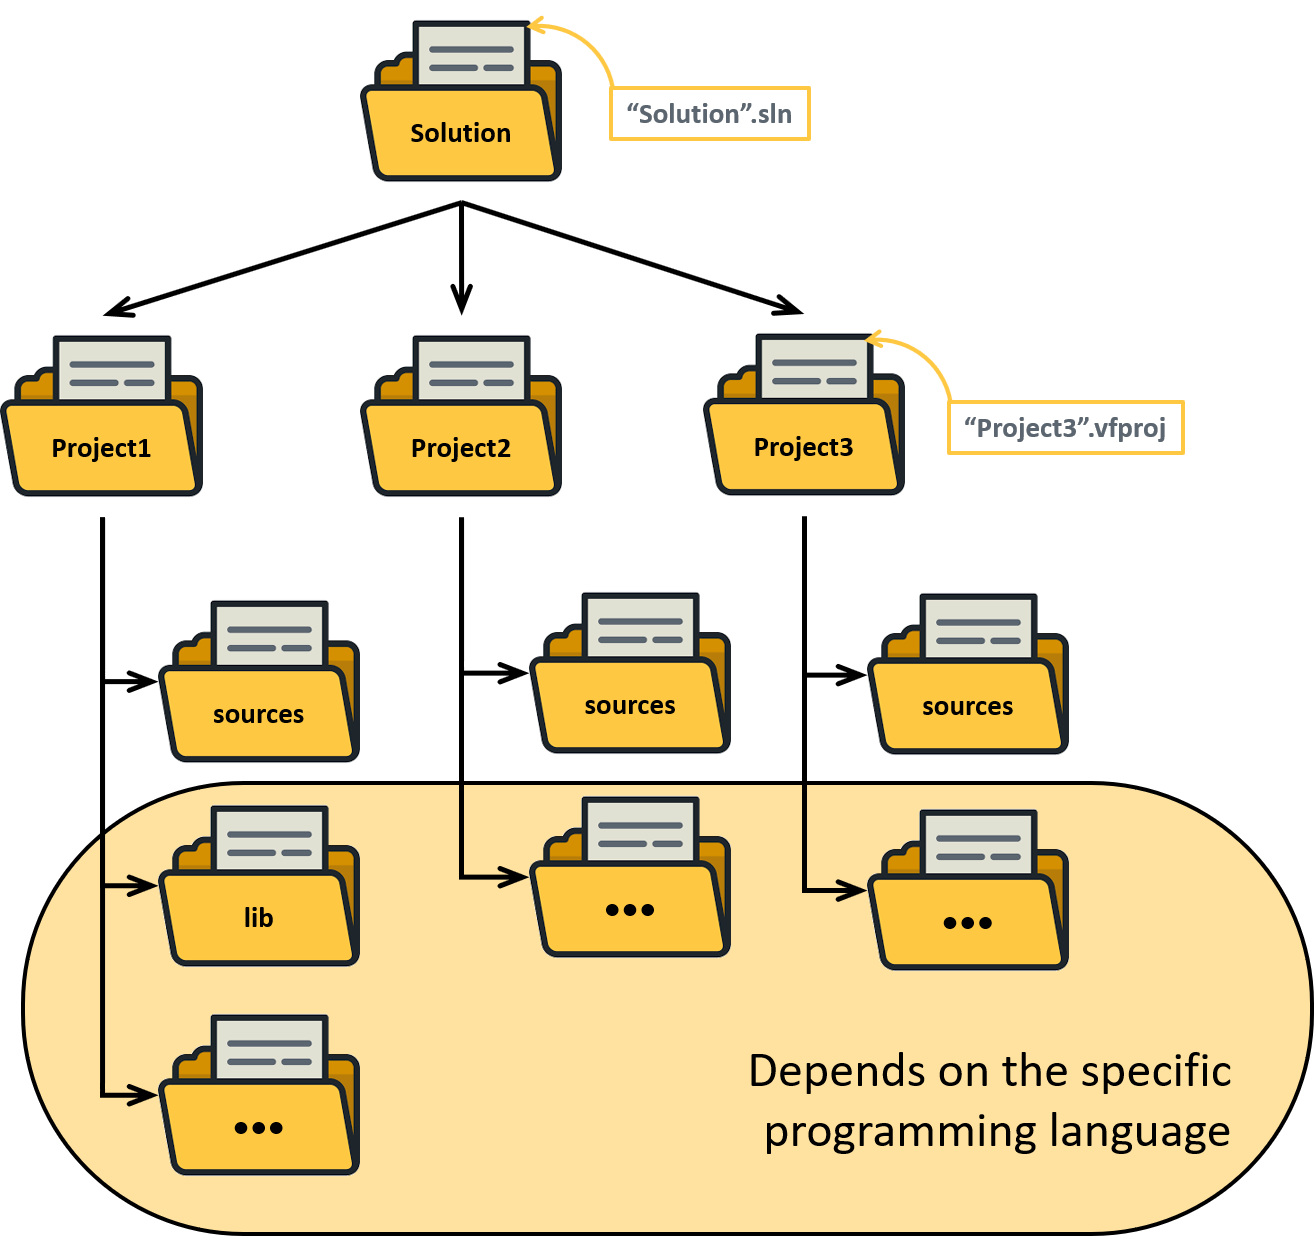
\includegraphics[width= \textwidth]{Figures/FolderScheme}
    \caption{Scheme of the main folders that we should have in a solution containing different projects.}
    \label{fig:FolderScheme}
\end{figure}

A program written in a human-readable programming language with our IDE is not understood by the computer. The Central Processing Unit (CPU) of the computer, in charge of the execution of the program, only processes machine code instructions which reduces the program to a number of very specific tasks in the registers of the CPU itself. The concepts of \textbf{Source} and \textbf{Object Codes} are essential. Both types of codes collect the computer instructions that conform our program. While the source code is written in a human-readable programming language, the object code is generated by the compiler and stores the program in a computer language like machine code (binary for example) or an intermediate language.

The different programming languages that exist store the mentioned codes in different types of files that can be distinguished by the file extension. Just as an example we will see that a source code written in Fortran language is stored in a \texttt{.f90} file while the object code generated by the compiler receives the extension of \texttt{.obj}. In the case of a C++ program, the source code can use the extension \texttt{.cpp} among others and the object code will be stored in the same extension as Fortran language (\texttt{.obj}). Apart from these files, a list of common used extensions can be found in a specific programming language (libraries, modules, images, scripts, etc.), this information is also treated during this guide.

%-----------------------
An important concept to handle is the difference between the \textbf{logical files/folders order} that is generated in our projects and the \textbf{real order} of the files and folders stored in the hard drive. In the first case, we add all the source codes, images, libraries, etc. to the project and we organize all the elements in the Solution explorer of the tool. We can create folders or move files as we want. However, each file can be stored anywhere in our hard drive, maybe in the folder of a different project/solution, in the desktop, in the cloud, etc. This is specially important for languages like Fortran where there is not relation between both schemes. We can add a library file to the logical folder called ``libraries'' while the real file is stored in our Desktop. The Fortran project will store the information about the location of the library. In addition, if we create a new file in that folder (using Visual Studio), it is by default stored in the project folder in the hard drive, but not necessarily in a folder called with the same name. The folders that organize all the necessary content for the program are different and we must manage not only the order used in the solution (seen in the solution explorer in Visual Studio) but also the real location of the files. %This behaviour forces us to know and control at all the time the files/folders structure in our project and the real structure in the hard drive.

It is not the same for languages like Python or JavaScript. Once the project is started, if we create a folder or a code file using Visual Studio, the same folder or file is created in our hard drive in the same location where our project and solution are (both projects and solutions are explained later). In this case we do not have to take an strict control of files since the structure is repeated and consistent. 

Let's think about a code file that we use in many different projects (stored in our desktop, outside our project folder, for example). If we are using Fortran, we can add that file to our project with no need of copying the file to the project folder. Different projects will have the path associated to the file and if we make a modification to the file, all the projects benefit from that update in the next compilation. Once again, this is different for languages like JavaScript. If we add the file to the project, a copy is automatically made in the project folder and a modification in the code stored in the desktop will be totally useless. If the file is used in 3 different projects, a modification in the code can become a mess. We strongly recommend to delete all files that has been previously copied to a project in order to avoid unnecessary duplications (there cannot be two files with the same name). If the code is going to be used in different projects we will build a library with that code (treated in each language) and include it in the different works.

\begin{IN}
    For all these reasons, we are going to follow the same files/folders scheme in our projects from now on. Whether it is automatically created or not, we have to store all the source codes in a folder called ``sources'' inside our folder project (see Figure \ref{fig:FolderScheme}). If the folder is not created by default in both the real and the logical folder scheme, we have to do it manually. In addition, a list of files and folders are created together with the source files in order to make the project work properly. These additional elements depend on the programming language we are using and they would be treated in the specific chapter. As a practical implementation of this topic, take a look at the example \ref{sec:Example2}.
\end{IN}
%-----------------------

Nevertheless, our programs are not only comprised by code files. Visual Studio works with the concepts of projects and solutions, each of them with their \textbf{configuration files and extensions associated}. It is important to clarify the nomenclature that the program gives to the project and solution files since we are going to live together with them from now on. Simplifying, it could be said that a \textit{project} is a specific program written in a programming language while a \textit{solution} is a set of different programs. In the official Microsoft Visual Studio documentation a project is defined as:

\begin{center}
    \begin{minipage}{0.7\linewidth}
        \vspace{3pt}
        {\small
            ``...In a logical sense, a project contains of all the source code files, icons, images, data files and anything else that will be compiled into an executable program or web site, or else is needed in order to perform the compilation. A project also contains all the compiler settings and other configuration files that might be needed by various services or components that your program will communicate with.''
        }
        \begin{flushright}
            (\url{https://msdn.microsoft.com/en-us/library/b142f8e7.aspx})
        \end{flushright}
        \vspace{3pt}
    \end{minipage}
\end{center}

\newpage
Related to solutions, the Visual documentation says: 

\begin{center}
    \begin{minipage}{0.7\linewidth}
        \vspace{3pt}
        {\small
            ``A project is contained, in a logical sense and in the file system, within a solution, which may contain one or more projects, along with build information, Visual Studio window settings, and any miscellaneous files that aren't associated with any project. In a literal sense, the solution is a text file with its own unique format; it is generally not intended to be edited by hand.
            
            A solution has an associated *.suo file that stores settings, preferences and configuration information for each user that has worked on the project.''
        }
        \begin{flushright}
            (\url{https://msdn.microsoft.com/en-us/library/b142f8e7.aspx})
        \end{flushright}
        \vspace{3pt}
    \end{minipage}
\end{center}

%-----------------------

%-----------------------

Both the solution and the project have files associated. The file where the solution is stored has \texttt{.sln} extension and contains information that the environment uses to load it, load the projects within the solution and other information attached. As an example, we can find there the file format version, the newest version of Visual Studio that saved the file, the older version of VS that can open the solution and a list of parameters needed for loading the project files. In the case of the project, the extension of the file depends on the programming language used. If an Intel Fortran project has been created, the extension is \texttt{.vfproj} while in the case of a C++ compiler, \texttt{.icproj} would be the extension. This file stores information about the configuration of the project in the different building modes; Release, Debug and those created by us. It also stores the name and relative path of all the files needed for opening and building the project and the admitted extensions that can be opened. 

The solution and project files are XML files (Extensible Markup Language), this means that the data structure is machine-readable and human-readable at the same time. Although both kind of files are automatically generated by Visual Studio and they are not made for being modified by hand, we can do it if required. We could open the file with a text editor, read the information and change parameters directly with no need of using VS. The solution settings for each user are stored in the \texttt{.suo} file that Visual Studio automatically creates when the solutions is saved. Unlike the mentioned files, this one is stored in a binary format so it is not human-readable and can not be modified by hand. 

All the configuration files mentioned are physically stored in our hard drive, in the folder reserved for the solution and the projects.




\FloatBarrier
\section{Example 1} \label{sec:Ex2}

In order to help the reader in the first steps with Visual Studio, a repository has been created in GitHub with the solutions and projects explained here. Apart from the examples created in the guide, some extra content can be found, specially in the fields of Applied Maths, Simulation software with Fortran, Energy efficiency in buildings or Embedded software (C++). The repository is located in the url: \url{https://github.com/jahrWork} (Figure \ref{fig:repository}).

\begin{figure}
    \centering
    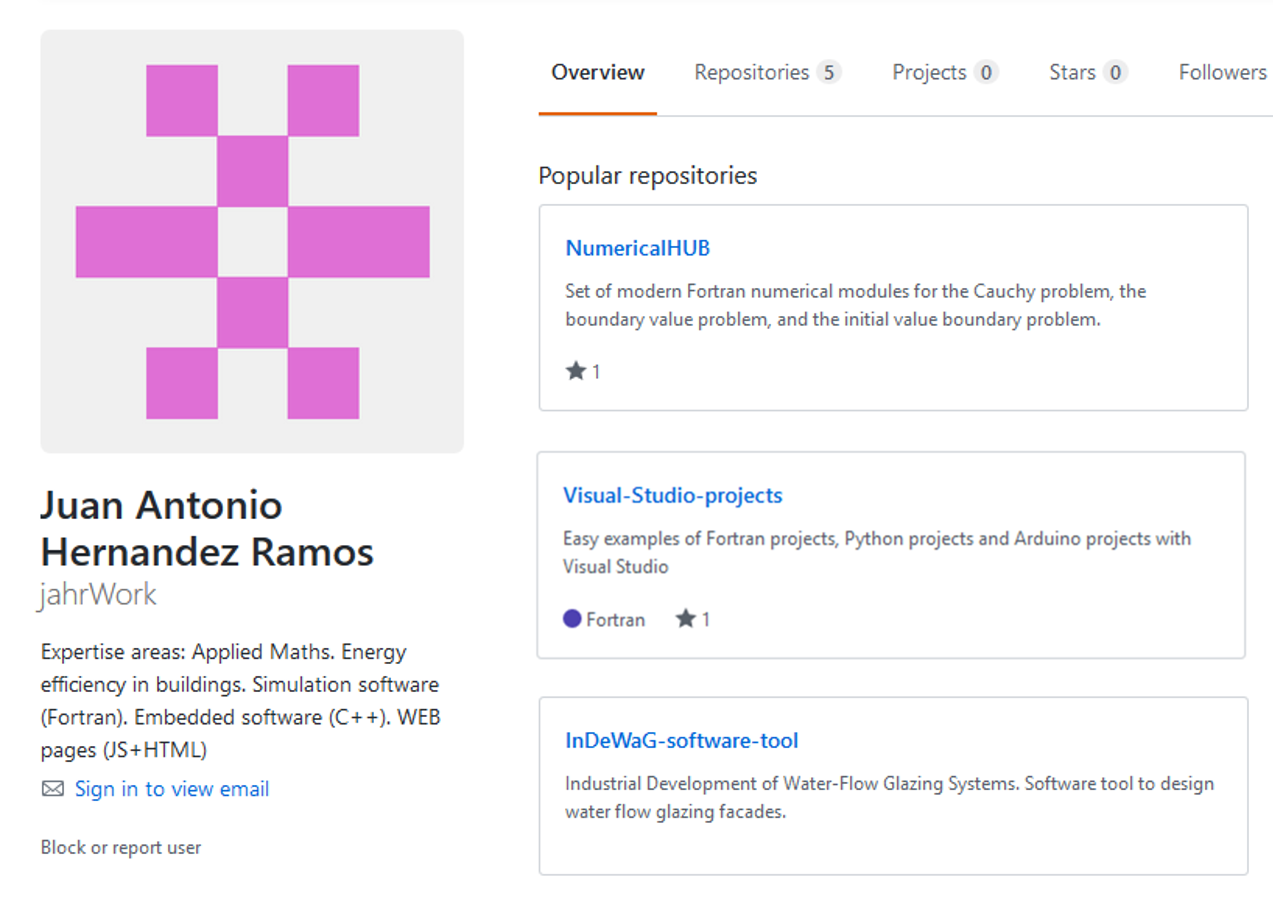
\includegraphics[width= \textwidth]{Figures/repository2}
    \caption{jahrWork repository in GitHub created by Juan Antonio Hernandez Ramos.}
    \label{fig:repository}
\end{figure}

Let's download, open and execute an example of this repository in order to get familiar with the solutions and projects. Follow these steps:

\begin{enumerate}[nosep]
    \item Open the url of the repository in your browser.
    \item Click on \textit{Visual-Studio-projects}.
    \item Click on the green button (\textit{Clone or download}) and click on \textit{Download ZIP}.
    \item In the folder where the ZIP file has been downloaded, unzip the folder and open it. 
    \item Double click on \texttt{Projects.sln} in order to open the solution in Visual Studio. If you just want to open the projects of a specific language, open the folder you want and double click on the \texttt{.sln} file.
    \item You find in the Solution Explorer a mix of projects in different programming languages, make right click on \textit{MainFortranGraph} and click on \textit{Set as StartUp Project} in order to select this project as the execution by default when clicking on the start button.
    \item Click on \textit{BUILD/Build MainFortranGraph} and wait until VS finishes.
    \item Click on \textit{DEBUG/Start Without Debugging} or press \texttt{Ctrl+F5}. The result of the execution is the plot of a sine curve.
\end{enumerate}
 

\FloatBarrier
\section{Example 2} \label{sec:Example2}

It is assumed now that a working version of Visual Studio is already installed in your computer (see chapter \ref{ch:VS}). In this section we create a unique solution called ``Semester1'' and as many projects as milestones have to be completed during the semester. We use Fortran language so the proper compiler must be already installed (see chapter \ref{sec:FortranIns}). The files and folders structure mentioned above is used for this example. 

Follow these steps:

\begin{enumerate}[nosep]
    \item Open your installed version of Visual Studio.
    \item Click on \textit{File/New/Project...} (Figure \ref{fig:Pro1}).
    \item In the \textit{Intel(R) Visual Fortran} menu select \textit{Console Application} and then click on \textit{Main Program Code}.
    \item Write the name of the first project to create in the field \textit{Name}, e.g. ``Milestone1''. Notice that the solution gets the same name by default. 
    \item Change the \textit{Location} of the solution, a directory will be created there.
    \item Write now the name of the solution ``Semester1'', it does not have to be the same as the name of the project (Figure \ref{fig:Intro1}).  
    \item Select the option \textit{Create directory for solution}.
    \item Click on \textit{OK}.
\end{enumerate}

\begin{figure}
    \centering
    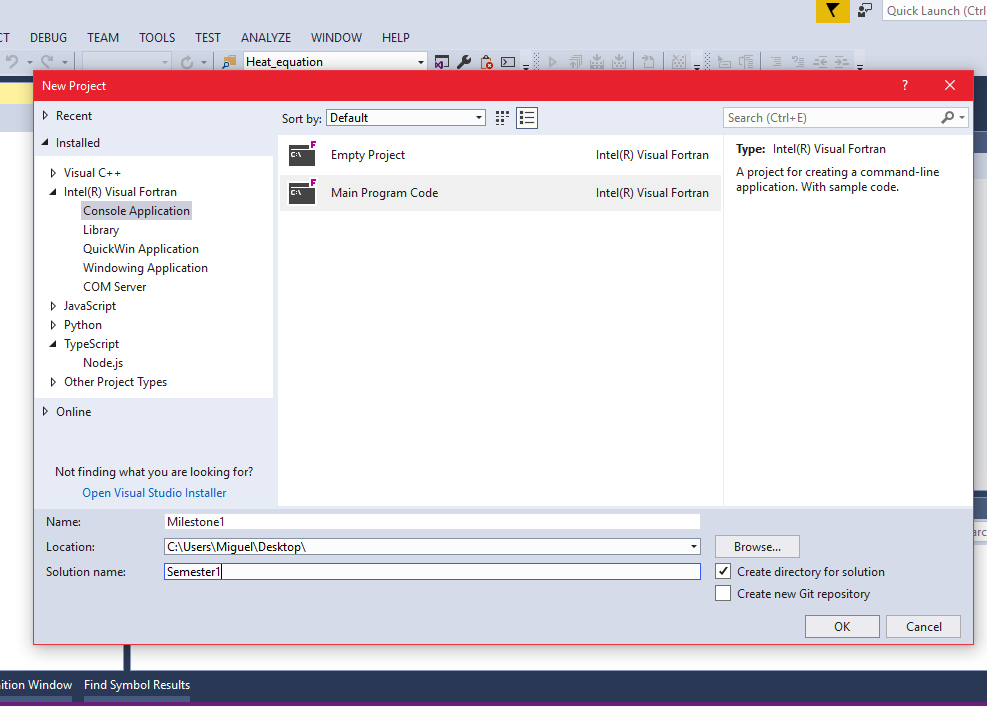
\includegraphics[width= 0.9\textwidth]{Figures/Intro1}
    \caption{Creation of a Fortran project within a solution in Visual Studio.}
    \label{fig:Intro1}
\end{figure}

Open now the path where your new solution has been created and open your solution folder. You find a \texttt{.sln} file with the name ``Semester1'' and a folder \texttt{Milestone1} containing the project data. Right now in this project folder you have a file \texttt{Milestone1.vfproj} with the configuration of the project, this configuration data is read by VS when the solution is opened. In addition, the first source code file \texttt{.f90} (with the same name of the project) has been created.

The folders structure is really different in the Solution Explorer of Visual. Three folders appear inside the project domain: \textit{Header Files}, \textit{Resource Files} and \textit{Source Files}. The last one contains the file \texttt{Milestone1.f90} mentioned above, with the main program code in Fortran (the Figure \ref{fig:Intro2} shows the initial structure of folders and files). In this code the ``Hello World'' example is already written so we can build the project and execute it without debugging. The results will be printed in a command window. 

\begin{figure}
    \centering
    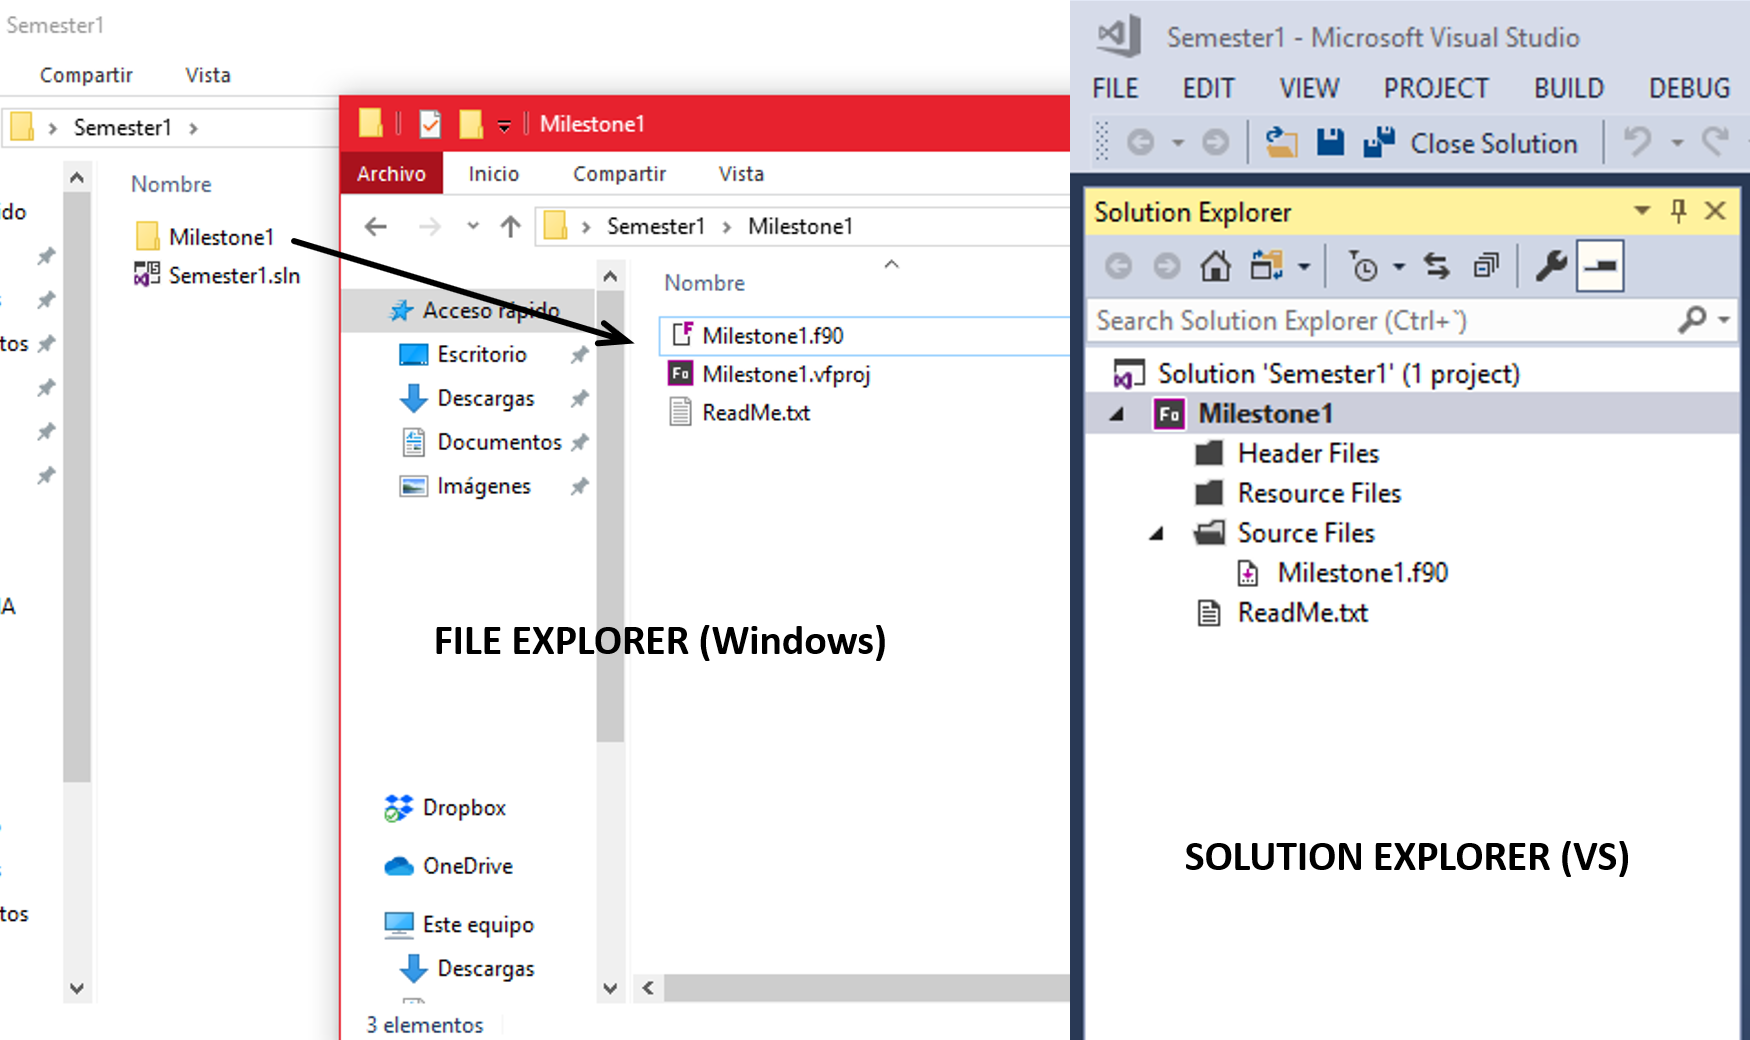
\includegraphics[width= 0.9\textwidth]{Figures/Intro2}
    \caption{Initial folders and files structure in the File Explorer of Windows and the Solution Explorer of Visual Studio.}
    \label{fig:Intro2}
\end{figure}

However, our first project is going to grow and some files and folders will be created. The following steps show how to imitate the structure seen in the Figure \ref{fig:FolderScheme} in order to maintain a strict folder order. 

\begin{enumerate}[nosep]
    \item Open in the File Explorer of Windows OS the project folder:
    
        \texttt{...\textbackslash Semester1\textbackslash Milestone1}.
    
    \item Create there a folder called ``sources''. This folder will contain all the source codes of your program. 
    \item Still using the File Explorer of Windows OS, cut the file \texttt{Milestone1.f90} and paste it inside the recently created folder. The Figure \ref{fig:Intro3} shows the final structure of folders and files.
    \item If you try to open this file in VS (double click on the name of the file in the Solution Explorer of the IDE), you will receive an error since the file is not in the initial location anymore. 
    \item Remove this file in the Solution Explorer by making right click on the name of the file and pressing \textit{Remove} and then clicking on \textit{Remove} once again.
    \item Make right click on the name of the folder \texttt{Source Files} in the Solution Explorer and click on \textit{Add/Existing item...}. Open ``sources'' and select \texttt{Milestone1.f90}. The file is once again in the project but with the new location. 
    \item From now on, all your codes can be stored in the same file ``sources'' (referring to the real order of the files) and they all can be stored in ``Source Files'' (logical order seen by the Solution Explorer). 
\end{enumerate}

Finally, all the projects to be created during the rest of the semester (Milestone2, Milestone3, etc.) can be stored in the same solution. The section \ref{sec:Include} tells how to include new projects and files in a solution already created. At the end of the semester you will have something like the Figure \ref{fig:Intro4}.

\begin{figure}
    \centering
    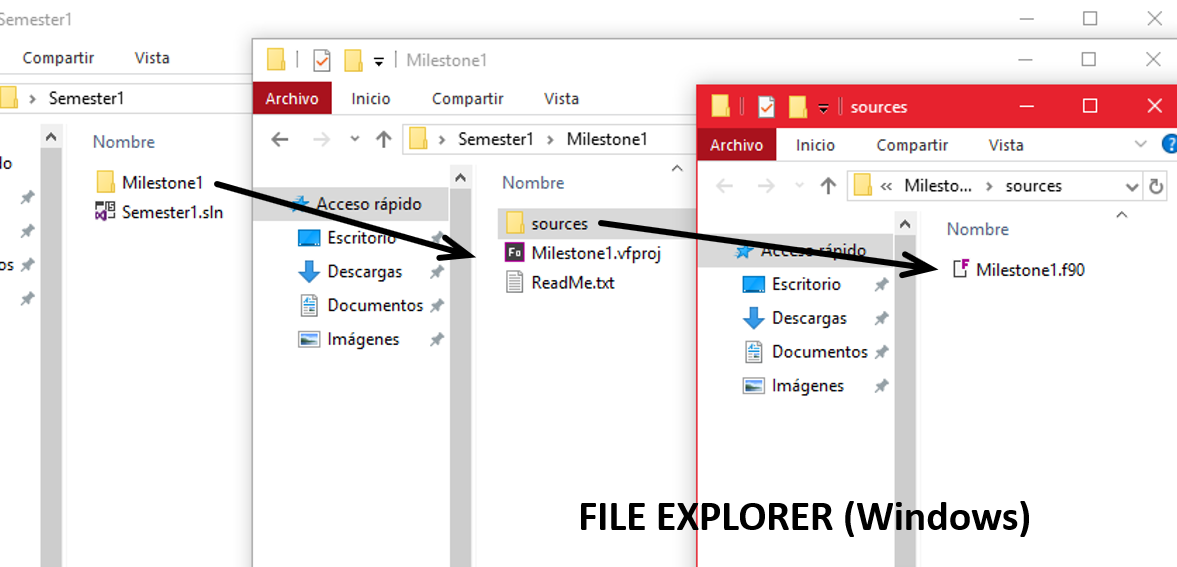
\includegraphics[width=  \textwidth]{Figures/Intro3}
    \caption{Folders and files structure in the File Explorer of Windows after organizing the Fortran project.}
    \label{fig:Intro3}
\end{figure}

\begin{figure}
    \centering
    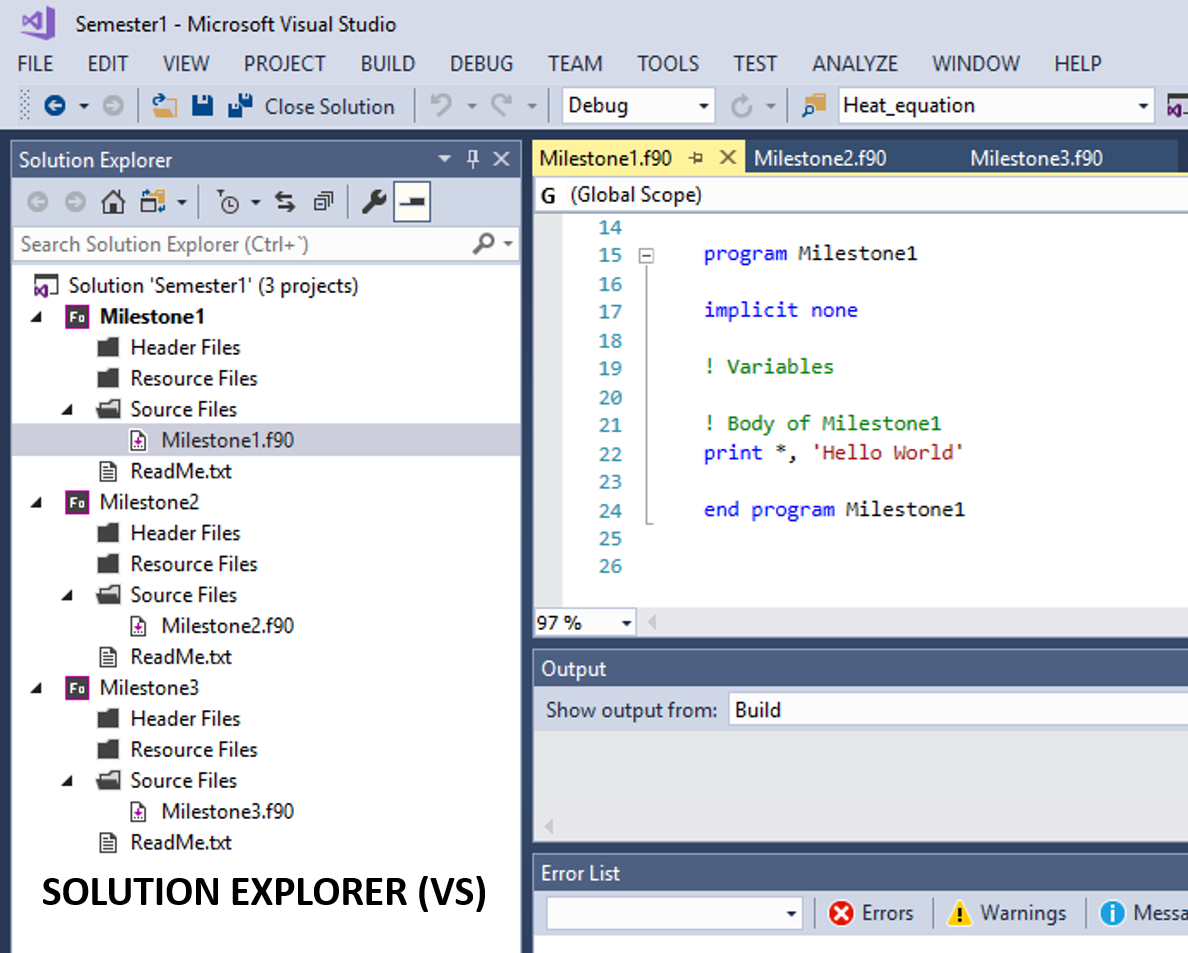
\includegraphics[width= \textwidth]{Figures/Intro4}
    \caption{Folders and files structure in the Solution Explorer of Visual Studio after creating three projects in the same solution.}
    \label{fig:Intro4}
\end{figure}






    
    \chapter{Visual Studio} \label{ch:VS}

    \FloatBarrier
    \section{Installing Visual Studio}

The first thing we are going to do is to install the latest version of Visual Studio, the IDE, in our computer. We have to \textbf{download the installer} of the program in the tab \textit{Downloads} of the official website (\url{https://visualstudio.microsoft.com/es/downloads/}). There, Microsoft offers the installers for the Community, Professional and Enterprise versions\footnote{In the same webpage Microsoft give us the possibility of downloading another tool: Visual Studio Code. In the introduction of this guide we explain why we use Visual Studio instead of this editor.}. Please notice that Professional and Enterprise releases have to be paid in case no license is obtained. However, the Community version is free and it is enough in most of the cases for the use we are going to make. If you are interested in the \textbf{VS Enterprise distribution} see how to install it with an academic license in the section \ref{sec:Enterprise}.

\begin{IN}
    \begin{itemize}
        \item Please notice that Visual Studio \textbf{MUST be installed in the first place}. The compilers, interpreters and extensions needed will be included later and with them all the tools that ensures the compatibility with all releases of Visual Studio installed in the computer.
        \item The examples of this book are created using Visual Studio 2017 and 2019. Typically, the Microsoft webpage offers the latest version of the IDE, however, you will find a previous distribution to download in case your computer is running an older Windows version (like Windows 8 for example).
    \end{itemize}
\end{IN}

When opening the url we quickly find the section reserved for the last release of Visual Studio (see Figure \ref{fig:VisualDownload}). In case the Visual Studio downloads are not shown, we can look for it by scrolling down the webpage or writing ``Microsoft Visual Studio'' in the space reserved for the search of downloads. We can obtain the installer of the Community version by clicking on \textit{Free Download }in that distribution.  A file is downloaded on our computer, the name should be something similar to \texttt{vs\_yyyyyyyy\_xxxxx.exe} where the distribution appears instead of ``y'' and a number of version appears in the place of the ``x''. We have chosen the Community version so we obtain a file similar to \texttt{vs\_community\_\_2074385403.1558468341.exe}. In case a more complete IDE version is needed, later it is explained how to obtain a student license and download the Enterprise distribution of the tool.

\begin{figure}
    \centering
    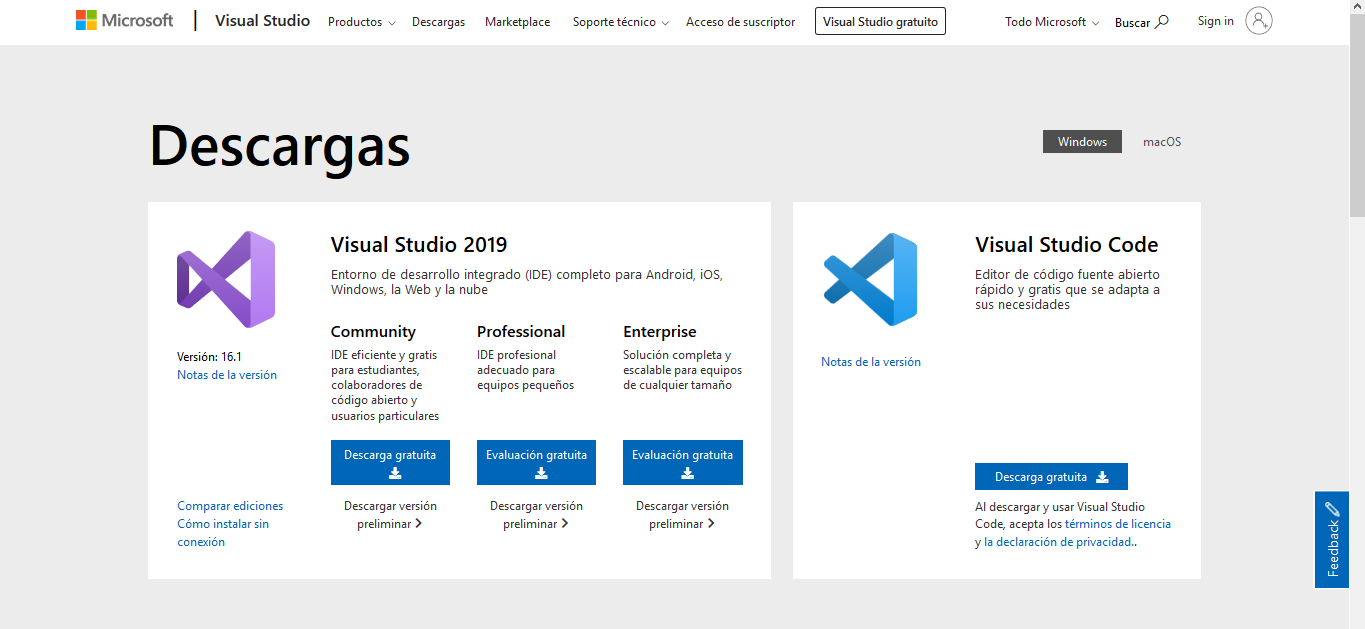
\includegraphics[width= \textwidth]{Figures/VisualDownload}
    \caption{Downloads tab of Microsoft Visual Studio webpage where the different installers for the distributions available can be downloaded.}
    \label{fig:VisualDownload}
\end{figure}

\newpage
Installing Visual Studio Community version:

\begin{enumerate}
    
    \item Execute the installer you have obtained. Accept first that the execution is done as an administrator and later accept the privacy conditions and the terms of the license of the software by clicking on \textit{Continue}. Wait for the program to download and start installing (see Figures \ref{fig:Instalacion-1} and \ref{fig:Instalacion0}).
    
    \item When finished, some options will appear in a window. There are four different tabs: Workloads, Individual Components, Language Packages and Installation folder. This tool called Visual Installer is essential for obtaining compilers and other tools used with different programming languages. In Workloads we choose \textit{Desarrollo para el escritorio con C++} and in Language Packages we choose: English or both Spanish and English (see figure \ref{fig:Instalacion1}).
    
    \item Click on \textit{Install} and wait (it might be slow).
    
    \item Once finished close all windows and restart the computer.
    
%    \item Execute Visual Studio. The first time some welcome windows appear (see figure \ref{fig:Instalacion2}), first we are going to Start Session. Although Community distribution is free for the people we first obtain a license for 30 days. In order to activate the product we have to initiate session. Click on Initiate Session. In the window that appears use your institutional email (finished with \textit{@alumnos.upm.es}), you will be redirected to the organization's sign-in page of the UPM. There you have to write again the same email and the password for that account and confirm the process. A webpage with the header ``Servicio de Identidad de RedIRIS'' may appear.
    \item Execute Visual Studio. The first time some welcome windows appear (see figure \ref{fig:Instalacion2}), first we are going to Start Session. Although Community distribution is free for the people we first obtain a license for 30 days and we have to initiate session in order to activate the product. Click on Initiate Session and in the new window that appears use your Microsoft account or your institutional email\footnote{If you use the institutional email of the UPM (finished with \textit{@alumnos.upm.es}), you will be redirected to the organization's sign-in page of the UPM. There you have to write again the same email and the password for that account and confirm the process. A webpage with the header ``Servicio de Identidad de RedIRIS'' may appear.}, in case you do not have a Microsoft account create it using the available link: \textit{Create one!}.
    
    \item Now the IDE starts to configure everything so it can take awhile. An Start window appears but you can click on \textit{Continue without code} and you access directly to the environment.
    
%    \item Notice that in the top right part of the IDE it is shown that you have already started session. If you click on the letter of your name and ``Account Configuration'' (see figure \ref{fig:Instalacion3}) you will see that your credentials are activated. In the right part of that window it may say that you are using a 30 days license, click on ``Search for an updated license'' and it automatically activate the product since you are using a personal session (see figure \ref{fig:Instalacion4}). 
    \item Now you have to check if the product is already activated with a license. Notice that the initial of your name appears in the top right part of the IDE so you have already started session. If you click on the letter of your name and \textit{Account Configuration} (see figure \ref{fig:Instalacion3}) you will see that your credentials are activated. In the right part of that window it may say that you are using a 30 days license, click on \textit{Search for an updated license} and it automatically activates the product (see figure \ref{fig:Instalacion4}).
    
    \item Your IDE is ready to work now. 
    
\end{enumerate}

\begin{figure}
    \centering
    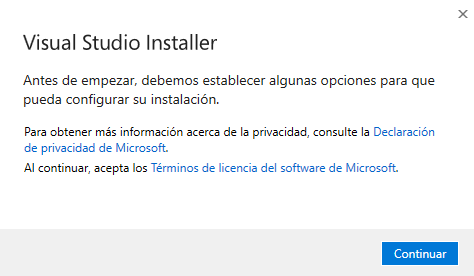
\includegraphics[width=  \textwidth]{Figures/Instalacion-1}
    \caption{First window that appears when executing the Visual Studio installer.}
    \label{fig:Instalacion-1}
\end{figure}

\begin{figure}
    \centering
    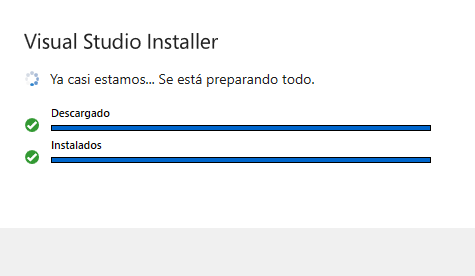
\includegraphics[width= \textwidth]{Figures/Instalacion0}
    \caption{Download and installation process of the Visual Studio environment.}
    \label{fig:Instalacion0}
\end{figure}

\begin{figure}
    \centering
    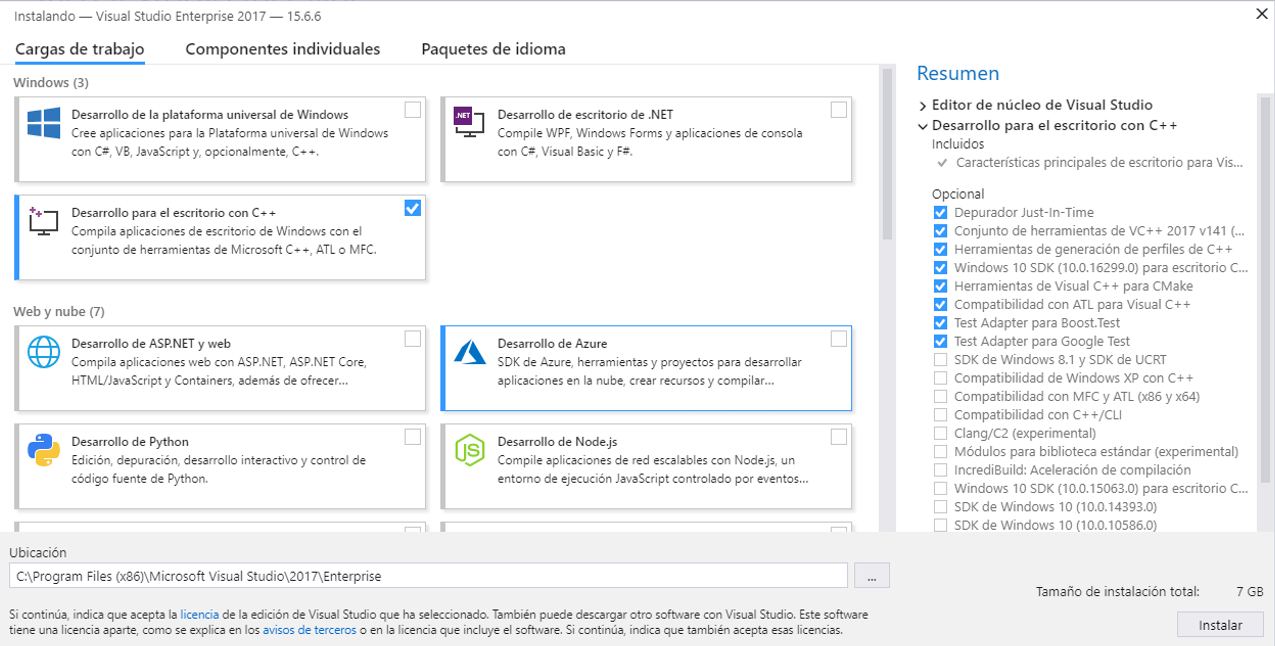
\includegraphics[width= \textwidth]{Figures/Instalacion1}
    \caption{Workload to be chosen in the installation process, \textit{desarrollo para el escritorio con C++} is selected in this step. In language package we choose at least English.}
    \label{fig:Instalacion1}
\end{figure}

\begin{figure}
    \centering
    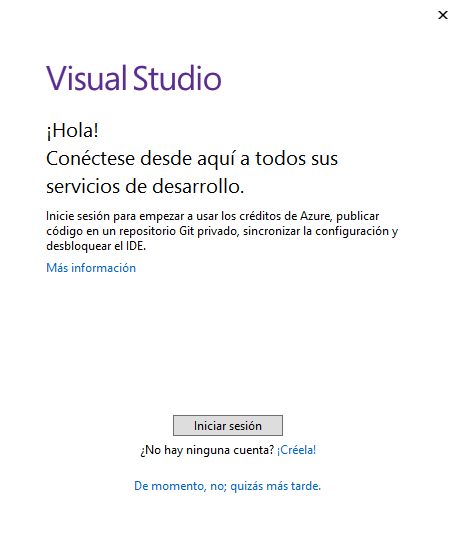
\includegraphics[width=0.7 \textwidth]{Figures/Instalacion2}
    \caption{Start window that appears after the installation, we have to start session now in order to use the options of Community version with no limit.}
    \label{fig:Instalacion2}
\end{figure}

\begin{figure}
    \centering
    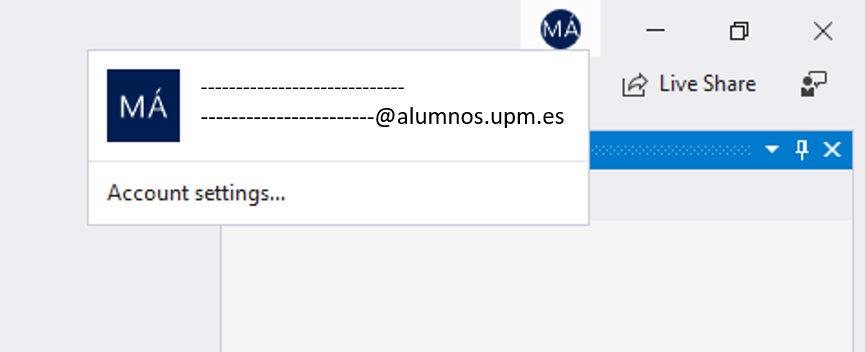
\includegraphics[width= \textwidth]{Figures/Instalacion3}
    \caption{Account Configuration inside the IDE, here we can activate the license and manage our accounts. You can use an institutional email or the Microsoft account.}
    \label{fig:Instalacion3}
\end{figure}

\begin{figure}
    \centering
    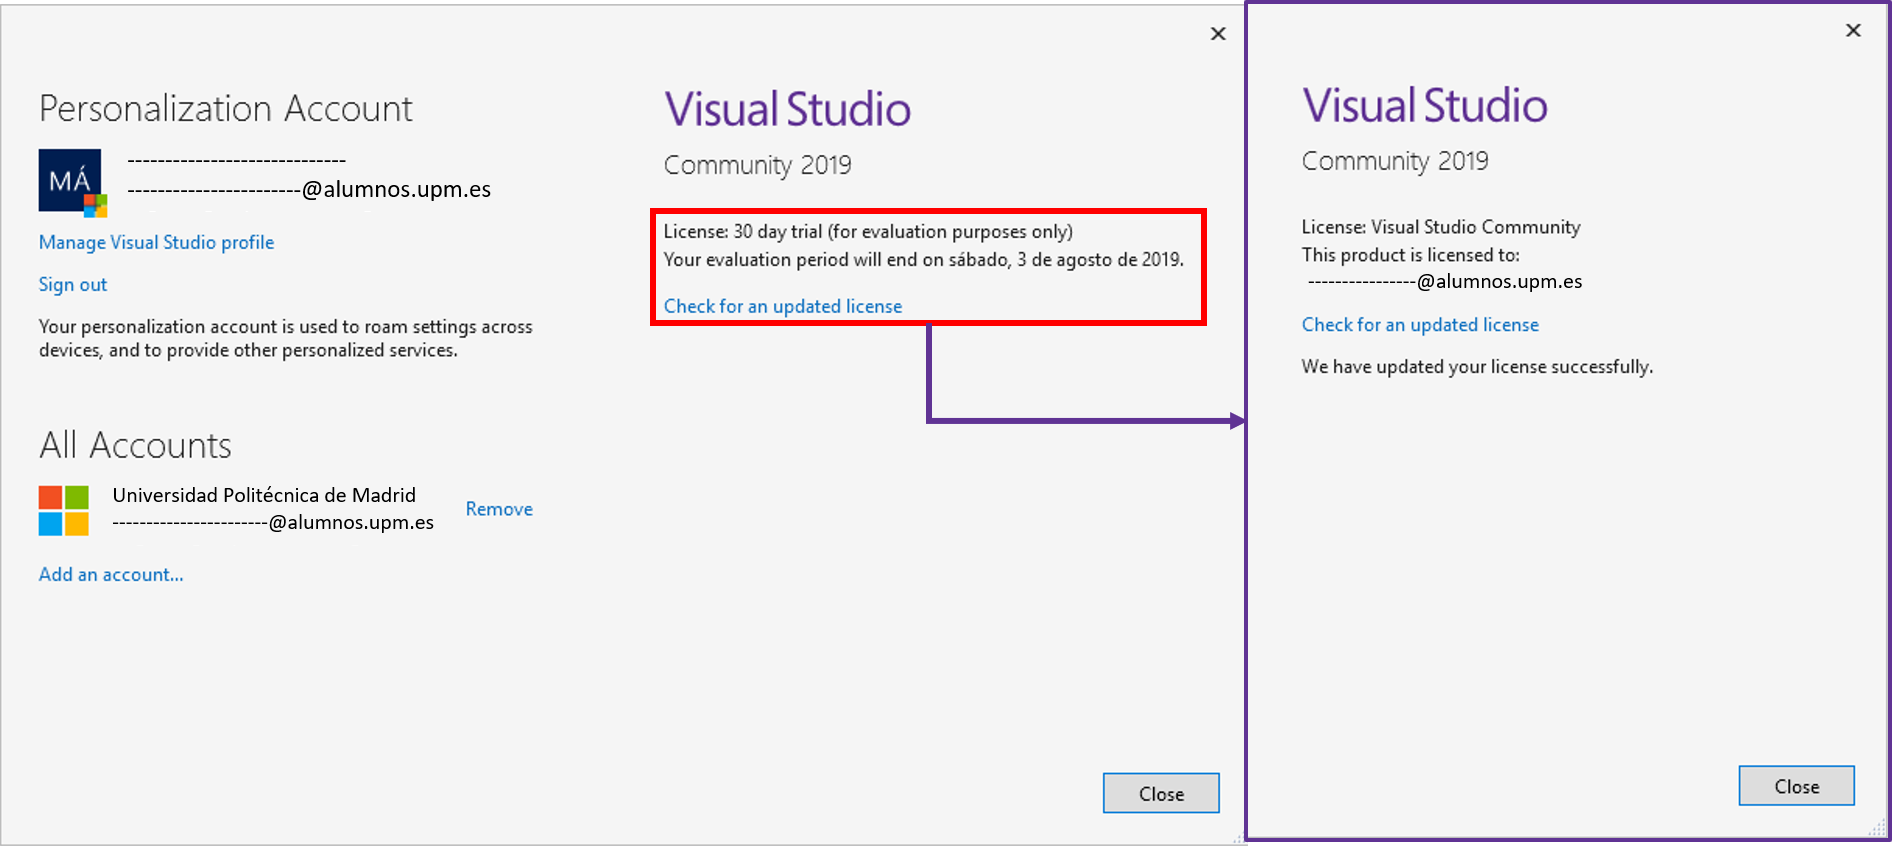
\includegraphics[width= \textwidth]{Figures/Instalacion4}
    \caption{Account Configuration menu, click on \textit{Search for an updated license} if your product is not already activated.}
    \label{fig:Instalacion4}
\end{figure}


Together with the environment itself, the \textbf{Visual Studio Installer} has been included in our computer, we can check it in the Start menu of Windows. We have seen this tool before during the process (Figure \ref{fig:Instalacion1}) and we are going to open it a few more times if we install all the programming languages and tools explained in this guide. For example, all the necessary tools needed for writing Cordova projects (smartphone applications) or the minimum templates used in a basic webpage can be installed using this installer.

It is interesting to become familiarized with the different ways of installing new functionalities, tools, extensions and updates in this IDE. First of all, we can use the \textbf{Visual Studio Installer} which can be opened through Windows OS using its shortcut as an administrator and also through the IDE by clicking on \textit{Tools/Get Tools and Features...}. Both ways show us the workloads that are already installed and the new functionalities available. We can also click on \textbf{\textit{Tools/Extensions and Updates...}} and navigate through the big amount of complements that appears. For example, the Arduino tool that is provided by \textit{Visual Micro} in order to write, upload, debug Arduino programs or burn microcontrollers with Visual Studio can be installed using this window. Finally, some programming languages like Python needs from the \textbf{installation of packages}, a topic that is treated further in the section \ref{sec:Python}.

\begin{IN}
    \begin{itemize}
        \item You are going to create a lot of projects in Visual Studio from now on. Even though the menu for creating projects is in the same place for all the programming languages (\textit{File/New/Project...}), we have noticed that the window that appears in the different versions of the IDE (2017 vs 2019 for example) differs. The fields to fill and the name of the available projects are the same but the menu is different; in Visual Studio 2017 you will find something like Figure \ref{fig:Pro2} while in the 2019 version something like Figure \ref{fig:C++1}.
        
        \item The Visual Studio installer has to be periodically updated. If you are going to install anything with the VS installer and a message appears when opening the tool, do not doubt in updating it by clicking on the pertinent option. Once finished you can resume the installation process. 
    \end{itemize}
\end{IN}


    \FloatBarrier
    \section{Configuring Visual Studio features} \label{sec:ConfigVS}

Now we are going to look through a list of useful functions and general common features that Visual Studio offers. All of them, when controlled, make the process of programming simpler:

\begin{enumerate}[nosep]
    \item Language
    \item Line numbers
    \item Navigation through files
    \item Look for references
    \item Open the definition of source functions and variables
    \item Show description of intrinsic and new functions
    \item Executing the program: \textit{Start without Debugging}
    \item Outlining blocks
    \item Additional requirements
    \item Common IDE configuration
    \item Windows inside the IDE
    \item Find in Files, Find and Replace
\end{enumerate}

\begin{enumerate}
	%%%%%%%%%%%%%%%%%%%%%%%%%%%%%%%%%%%%%%%%%%%%%%%%%%%%%%%%%%%%%%%%%%%%%%%%%%%%%%%%%C
	\item \textbf{Language}
	
	This manual has been written assuming that the IDE is configured in English, if you have used Spanish as default language, it can be changed in \textit{Tools/Options/International Settings}. There are options and commands with no intuitive translation to Spanish so we recommend getting used to the English version of the IDE and the English name of the programming concepts.
	
    
	%%%%%%%%%%%%%%%%%%%%%%%%%%%%%%%%%%%%%%%%%%%%%%%%%%%%%%%%%%%%%%%%%%%%%%%%%%%%%%%%%C
	\item \textbf{Line numbers} 
	
    %	Why showing line numbers is useful can be clear, but there are good practices that appear when our code is going to be shown in a text document (\LaTeX). It is useful to write before some subroutines, functions or other pieces of code a comment with the line number itself. For example, if our subroutine starts in the line 345, we can write a comment in that line saying ``this is the line 345''. Hence, the code is ``fixed'' in that position. We must not move it when expanding the program so it is interesting to reserve some space before and after every subroutine and function in case new lines have to be added. When writing documentation about our code in \LaTeX, it looks for the code and extracts some lines and the specific part of the program will always be in the same position among all the program.
    The line numbers are unique assignments for each of the code lines of your program (see Figure \ref{fig:LineNumbers}). This essential tool is used in all the programming languages mentioned in this guide, they are specially helpful when a list of errors appears in the compilation and each error must be found (in a specific file and line) in order to fix them. It is a good idea to change the configuration of the IDE to show them by default, independently of the language. Go to \textit{Tools/Options...} and in the menu \textit{Text Editor/All Languages/General} select the option \textit{Line numbers}. These numbers are also an easy way of referencing your code in case of writing documentation about it. 
    
    \begin{figure}
        \centering
        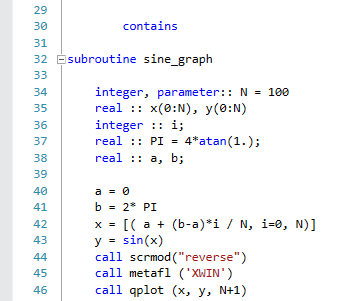
\includegraphics[width=0.7\textwidth]{Figures/LineNumbers}
        \caption{Example of the line numbers that leads all the code lines of a program.}
        \label{fig:LineNumbers}
    \end{figure}
	
	
    \newpage
	%%%%%%%%%%%%%%%%%%%%%%%%%%%%%%%%%%%%%%%%%%%%%%%%%%%%%%%%%%%%%%%%%%%%%%%%%%%%%%%%%C
	\item \textbf{Navigation through files}
	
	There are some basic functionalities that are very useful when managing big codes. The following features are activated by default in the IDE and both simplify the navigation across files. %others should be set in the configuration of Visual.
    
    \textbf{Navigation buttons:} \textit{Navigate Backward} and \textit{Navigate Forward} (Figure \ref{fig:Commands2}) have the same roles as Back and Forward in Windows OS but, instead of navigate across folders, we navigate across our opened and recently viewed codes.
    
    \begin{figure}
        \centering
        
\includegraphics[width= 0.3 \textwidth]{Figures/Commands2}
        \caption{Navigation buttons: \textit{Navigate Backward} and \textit{Navigate Forward}.}
        \label{fig:Commands2}
    \end{figure}
    
    
    %%%%%%%%%%%%%%%%%%%%%%%%%%%%%%%%%%%%%%%%%%%%%%%%%%%%%%%%%%%%%%%%%%%%%%%%%%%%%%%%%C
    \item \textbf{Look for references}
    
    Even more powerful tools when we navigate through codes are \textit{Go To Definition} and \textit{Find All References}. In order to enable the possibility of looking for all references, we click on \textit{Tools/Options.../Text Editor/Fortran/Advanced} and we select \textit{True} in the option \textit{Enable Find All References} (as can be seen in the Figure \ref{fig:Commands3}).
    
    \textbf{Find All References} function, as the name says, will look for the text we want in the whole project. If it is a variable, we can know how many times (and where) is used, changed, printed, etc. and if it is a subroutine we can find where is called and where is defined. In order to use it we have to click with the right button in the name of the element and click in this option.
    
    \begin{figure}
        \centering
        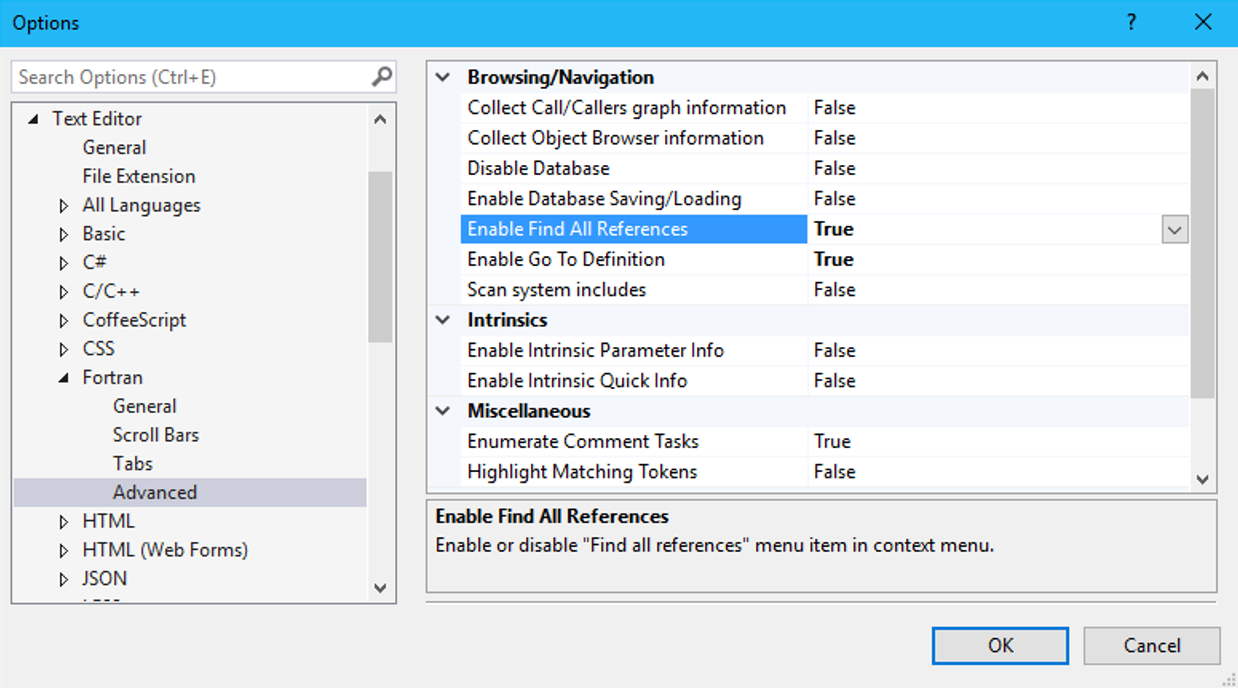
\includegraphics[width= \textwidth]{Figures/Commands3}
        \caption{\textit{Enable Find All References} and \textit{Enable Go To Definition} options to activate in the Visual Studio configuration.}
        \label{fig:Commands3}
    \end{figure}
    
    \begin{IN}
        Notice that Visual Studio has a very useful search engine that can be accessed with toolbars. The command needed is \textit{Find in files} or just \textit{Find} and it can also be minimised and put everywhere in the screen, ready to be used whenever. It is treated later in the item \ref{list:FIND}.
    \end{IN}
    
    \newpage
    %%%%%%%%%%%%%%%%%%%%%%%%%%%%%%%%%%%%%%%%%%%%%%%%%%%%%%%%%%%%%%%%%%%%%%%%%%%%%%%%%C
    \item \textbf{Open the definition of source functions and variables}
    
    Exactly like the previous tool, \textit{Go to Definition} function have to be enabled in \textit{Tools/Options.../Text Editor/Fortran/Advanced} and selecting \textit{True} in the option \textit{Enable Go To Definition} (see the Figure \ref{fig:Commands3}).
    
	\textbf{Go to Definition} function allows us to find the declaration of any variable in our code. If we for example manage a big program with multiple files and we do not know the meaning of a variable, we can click with the right button of our mouse in the variable and select this option. The window automatically moves to the line where the variable is declared, whether it is in the same file or in a different one (opening then the specific module or file with the declaration). If this tool is used with a subroutine or function, a different file will also be opened in a new window, showing then the definition of the requested piece of code. It is important to notice that, for example in the case of Fortran, it does not work if the subroutine is in a module or library already compiled but if we have included the source code in our project, we will be able to navigate quickly through files.
    
    
	%%%%%%%%%%%%%%%%%%%%%%%%%%%%%%%%%%%%%%%%%%%%%%%%%%%%%%%%%%%%%%%%%%%%%%%%%%%%%%%%%C
    \item \textbf{Show description of intrinsic and new functions}
	
	\textit{Enable Intrinsic Parameter Info} and \textit{Enable Intrinsic Quick Info} make faster the writing of code, both show quick information about functions and subroutines dynamically. To activate these features go to the menu \textit{Tools/Options.../Text Editor/Fortran/Advanced} and mark \textit{True} in the mentioned names (see Figure \ref{fig:Commands4}). The first one, \textbf{Enable Intrinsic Parameter Info}, ``\textit{displays the signature of an intrinsic in a tooltip when a user types the parameter list start character}''. This means that some essential information about the procedures and arguments will appear when typing a parenthesis after an intrinsic function or subroutine. The Figure \ref{fig:Commands5} shows an example with the cosine function. The second option, \textbf{Enable Intrinsic Quick Info}, displays intrinsic information and descriptions when we place the pointer over an intrinsic name. In the Figure \ref{fig:Commands6}, for example, a list of arguments associated to the subroutine is shown when the pointer stays on the function \texttt{Wave\_equation\_2D}.
	
	\begin{figure}
		\centering
		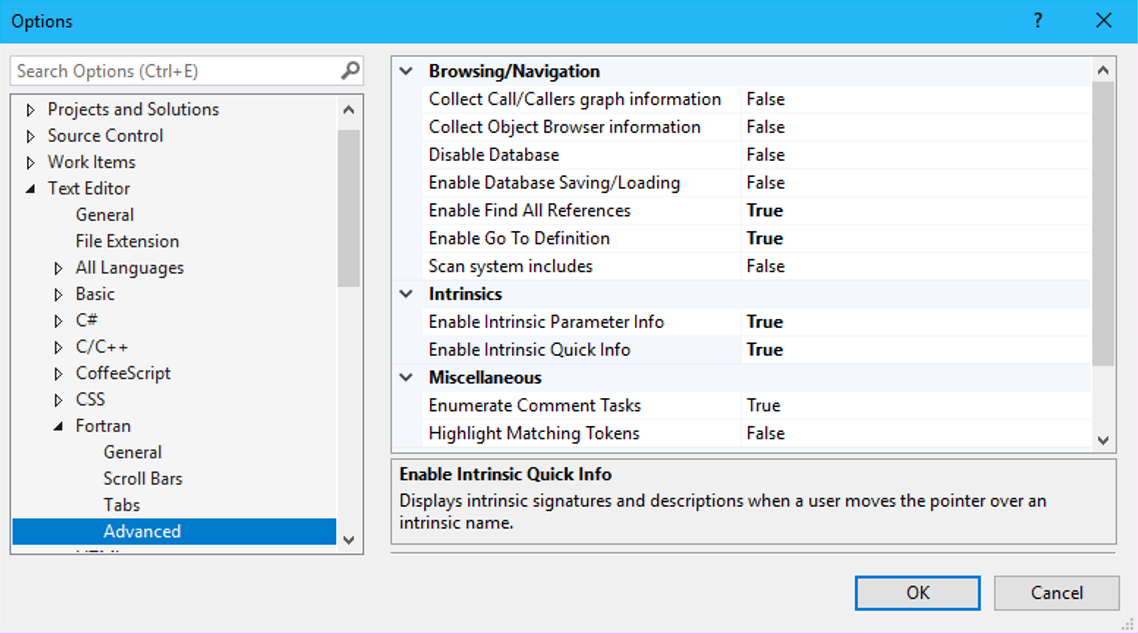
\includegraphics[width=  \textwidth]{Figures/Commands4}
		\caption{\textit{Enable Intrinsic Parameter Info} and \textit{Enable Intrinsic Quick Info} are both really useful when our codes become long and they are spread in multiple source files.}
		\label{fig:Commands4}
	\end{figure}
	
	\begin{figure}
		\centering
		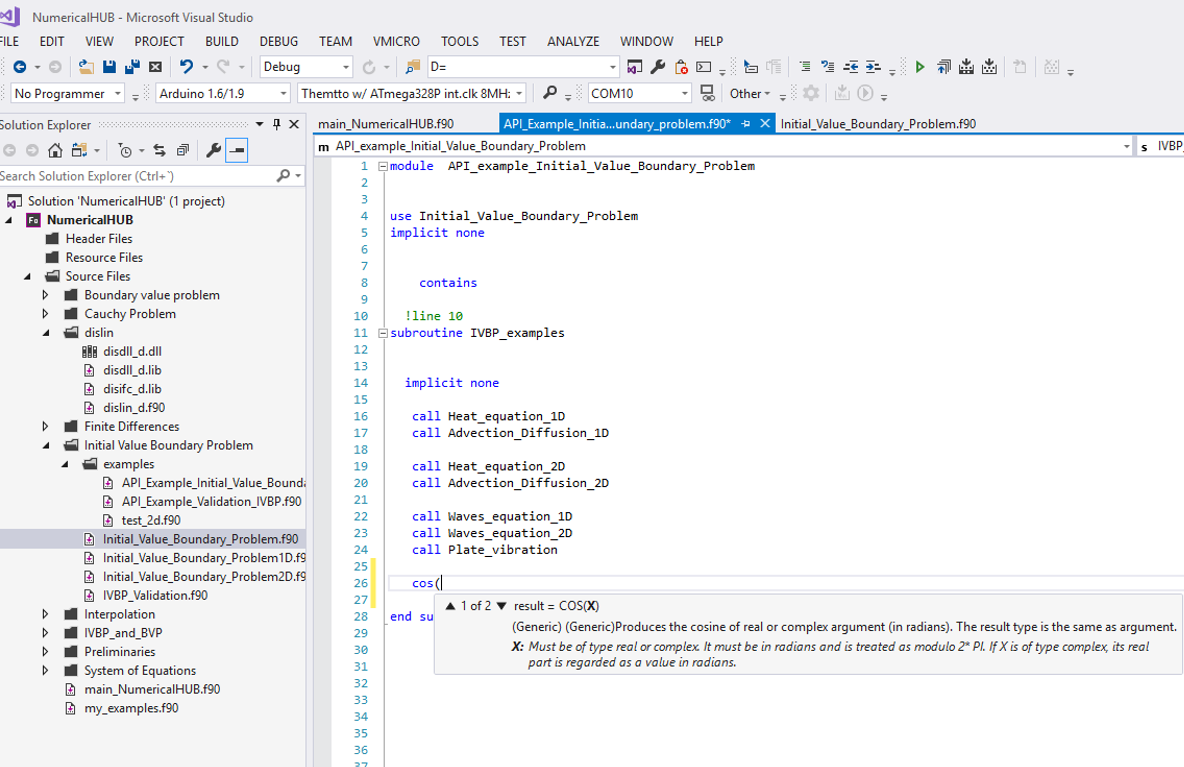
\includegraphics[width= \textwidth]{Figures/Commands5}
		\caption{Example of \textit{Intrinsic Parameter Info}.}
		\label{fig:Commands5}
	\end{figure}
	
	\begin{figure}
		\centering
		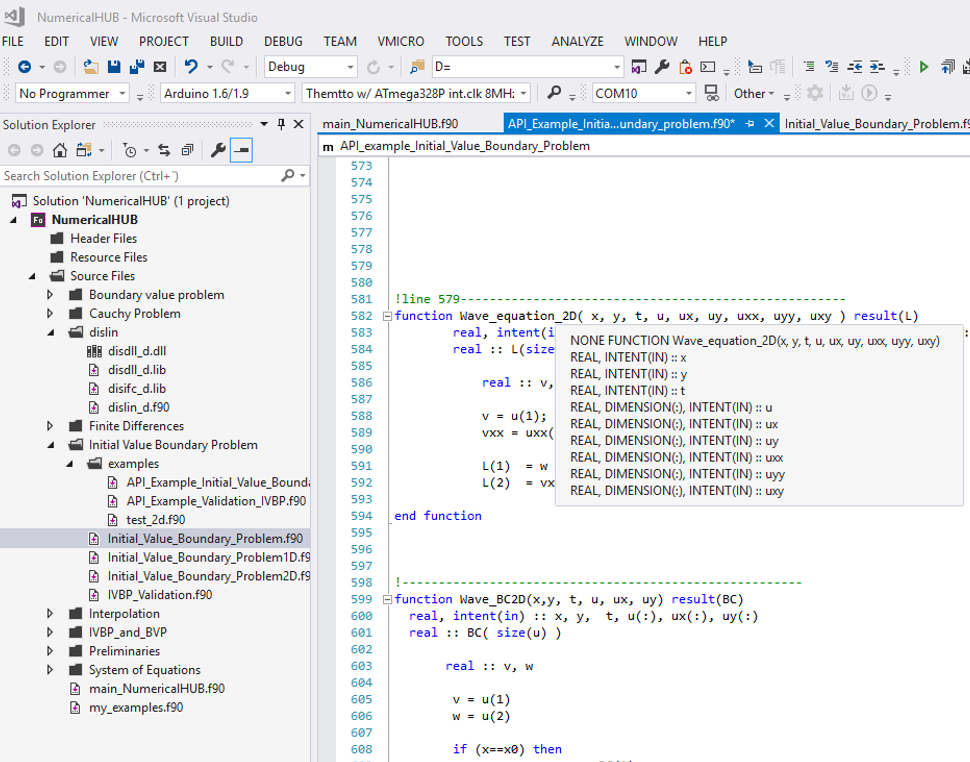
\includegraphics[width= \textwidth]{Figures/Commands6}
		\caption{Example of \textit{Intrinsic Quick Info}.}
		\label{fig:Commands6}
	\end{figure}
	
    
    \FloatBarrier
    %%%%%%%%%%%%%%%%%%%%%%%%%%%%%%%%%%%%%%%%%%%%%%%%%%%%%%%%%%%%%%%%%%%%%%%%%%%%%%%%%C
    \item \textbf{Executing the program: \textit{Start without Debugging}}
    
    This essential command of Visual Studio allows to \textbf{run the application/program} in all the different programming languages treated here. Once the program is written it can be executed by clicking on \textit{DEBUG/Start without Debugging}, pressing \textit{Ctrl+F5} or pressing the icon
    
    %\raisebox{-\mydepth}{\fbox{
\includegraphics[height=2\myheight]{Figures/StartSymbol}}}
    \begin{figure}[H]
        \centering
        
\includegraphics[width= 0.1\textwidth]{Figures/StartSymbol}
        %\caption{Example of \textit{Intrinsic Quick Info}.}
        %\label{fig:Commands6}
    \end{figure}
    
    of your toolbars. If you cannot see the mentioned icon in your toolbars take a look at the section \ref{sec:Shortcuts}.
    
    Notice that Visual Studio will launch your application without attaching the Debugger, you won't be able to pause the execution by breakpoints or use default debugging tools of the IDE. However, this is by far the most common method for executing programs in this guide. The behaviour of the command depends on the specific language used. For example, in Fortran it \textbf{saves} the modified files, \textbf{compiles}, \textbf{links} and \textbf{executes} all the project selected in the Solution Explorer. By contrast, in Python this command invokes the interpreter and the code is read and interpreted so the results can be shown in a command window.
    
    %%%%%%%%%%%%%%%%%%%%%%%%%%%%%%%%%%%%%%%%%%%%%%%%%%%%%%%%%%%%%%%%%%%%%%%%%%%%%%%%%C
    \item \textbf{Outlining blocks}
    
    \textbf{Outlining the source code} is one of the most common code folding patterns that IDEs and code editors offer. This feature allows to collapse a code block to a single line normally based on the syntax of the specific language used (other mechanisms appear depending on the indentation, the tokens or the preferences of the user). In general, the user can hide and show pieces of code that define a structure e.g. functions, subroutines, loops, if statements, etc. Then the code can be easily managed (specially if there is a large amount of text in the program) since only the headers of the hidden block are seen. Getting an overview of code and navigating through is now easier without being distracted by other code. The Figure \ref{fig:Outlining} shows an example.
    
    \begin{figure}
        \centering
        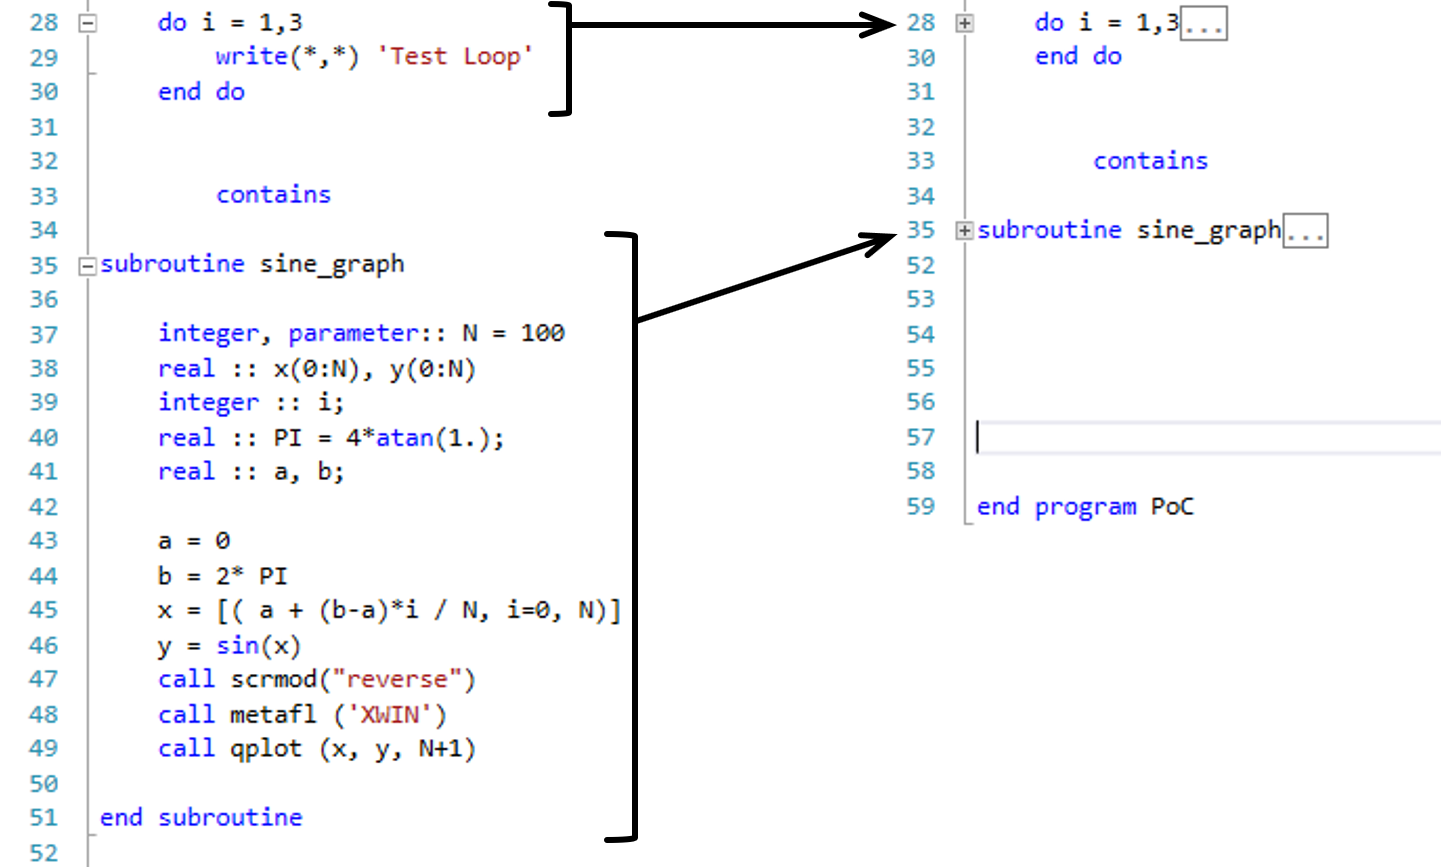
\includegraphics[width= \textwidth]{Figures/Outlining}
        \caption{Example of two pieces of code hidden by the user, one is a loop and the other a subroutine. By clicking on + or - we can deploy or hide the code.}
        \label{fig:Outlining}
    \end{figure}

    Depending on the language you are configuring the way to activate these features can vary, as an example we can go to \textit{TOOLS/Options.../Text Editor} and deploy the Fortran options. There click on \textit{Advanced} and in the menu called \textit{Outlining} mark \textit{True} in the options \textit{Enable Outlining} (which is actually activated by default) and \textit{Outline Statement Blocks} in case you also want to outline statements like loops. Notice that this options could be in a different menu for each programming language.
    
    If there is a piece of code where the outlining option does not appear automatically and you want to hide it, just do the following: select all the text to be outlined, right click on the selection, deploy \textit{Outlining} menu and click on \textit{Hide selection}. Then, that block of text can be shown and hidden on demand. 
    
    
    %%%%%%%%%%%%%%%%%%%%%%%%%%%%%%%%%%%%%%%%%%%%%%%%%%%%%%%%%%%%%%%%%%%%%%%%%%%%%%%%% 
    \item \textbf{Additional requirements}
    
    There are some tools that are common for a lot of Microsoft programs and in the case of the software development can be really useful. First of all, the different \textbf{extensions of the files} created in a software project are essential and the whole guide is full of references to some kind of files. Make sure that you have already activated in your Windows OS the option that shows the extensions of the files. If it is not activated, open any folder in your computer, click on \textit{View} and mark the option \textit{File name extensions}. From now on, you will see when a file is a C++ source code, a library or maybe a Fortran module.
    
    Part of the Visual Studio potential can be accessed using the \textbf{right button} of the mouse, exactly like the context menu of Windows OS. The options shown depend on the element where we deploy the pop-up menu and it is desirable to become familiarised with some commonly used functions. Just as an example, \textit{Go To Definition} and \textit{Find All References} will appear if we use the right button in the code (variables, calls to functions, intrinsic functions, etc.). If this button of the mouse is used in the solution explorer we can see different behaviour in the case of clicking on the name of projects and  the name of the solution. In the project the pop-up menu mainly shows the possibilities of Building, Rebuilding and Cleaning the project, adding folders or files and opening the properties of the project (which we will see in other chapters how important they are). However, in the name of the solution, the menu shows similar options but related to the whole solution (Build, Rebuild, Clean, Add existing or new projects, Rename the solution, open the solution properties, etc.). Try opening this menu in different places to get used to it.
    
    Exactly like in Windows OS we can make \textbf{bigger or smaller} what it is displayed in the screen, with the codes it is similar. Once you have your first piece of code opened in the IDE, try to make it bigger or smaller by pressing \texttt{Ctrl} and moving the scroll wheel of the mouse. The same effect could be achieved with the mouse pad.
    
    Finally, two different ways of \textbf{selecting pieces of code} can be used. The common way is pointing the cursor of the mouse in one line of the code, press \texttt{Ctrl+Shift} and click on a different part, all the lines between these two point will be selected. An useful alternative in order to select a vertical block of text is achieved by pressing the \texttt{Alt} key at the same time that the left button of the mouse and dragging the mouse in those lines we want to select.
    
    %%%%%%%%%%%%%%%%%%%%%%%%%%%%%%%%%%%%%%%%%%%%%%%%%%%%%%%%%%%%%%%%%%%%%%%%%%%%%%%%% 
    \item \textbf{Common IDE configuration}
    
    We can click on \textbf{\textit{Tools/Options...}} and start customizing the IDE in the \textbf{\textit{Environment}} menu. For example, the colour theme in the \textit{General} section (Dark, Light, Blue, etc.) or the auto-saving information frequency in the \textit{AutoRecover} tab can be decided here. We can also change the fonts and colours of the programming language or the default options for the \textit{Startup} (first window that appears when opening Visual Studio). 
    
    Since some compilers (e.g. GFortran) do not recognise tabs as characters, we could find warnings each time we compile a code with tabs instead of spaces. Hence, it is recommended to check that \textit{Insert Spaces} is marked in the \textit{Tabs} menu of the \textbf{\textit{Text Editor}} section (at least in the programming languages you are interested in).
    
    %%%%%%%%%%%%%%%%%%%%%%%%%%%%%%%%%%%%%%%%%%%%%%%%%%%%%%%%%%%%%%%%%%%%%%%%%%%%%%%%% 
    \item \textbf{Windows inside the IDE}
    
    Related to the different \textbf{windows} around the environment, the behaviour is the same as Windows OS. We can change position, make them fixed or floating, configure different options, etc. We can decide for each window in a little arrow located in the right upper part, also close those we do not need or open new ones in \textbf{\textit{View}} tab. \textit{Solution Explorer}, \textit{Properties Window}, \textit{Bookmark Window} or \textit{Output} are some windows we are going to need from now on. The Figure \ref{fig:Config1} shows an example of distribution of two essential windows: \textbf{Solution Explorer} and \textbf{Output}, we can choose our favourite position and move them. If we want to move the windows we grab it and Visual Studio will show us some default positions we could choose, we just have to drop it in the little boxes shown (or drop it in a floating point).
    
    \begin{figure}
        \centering
        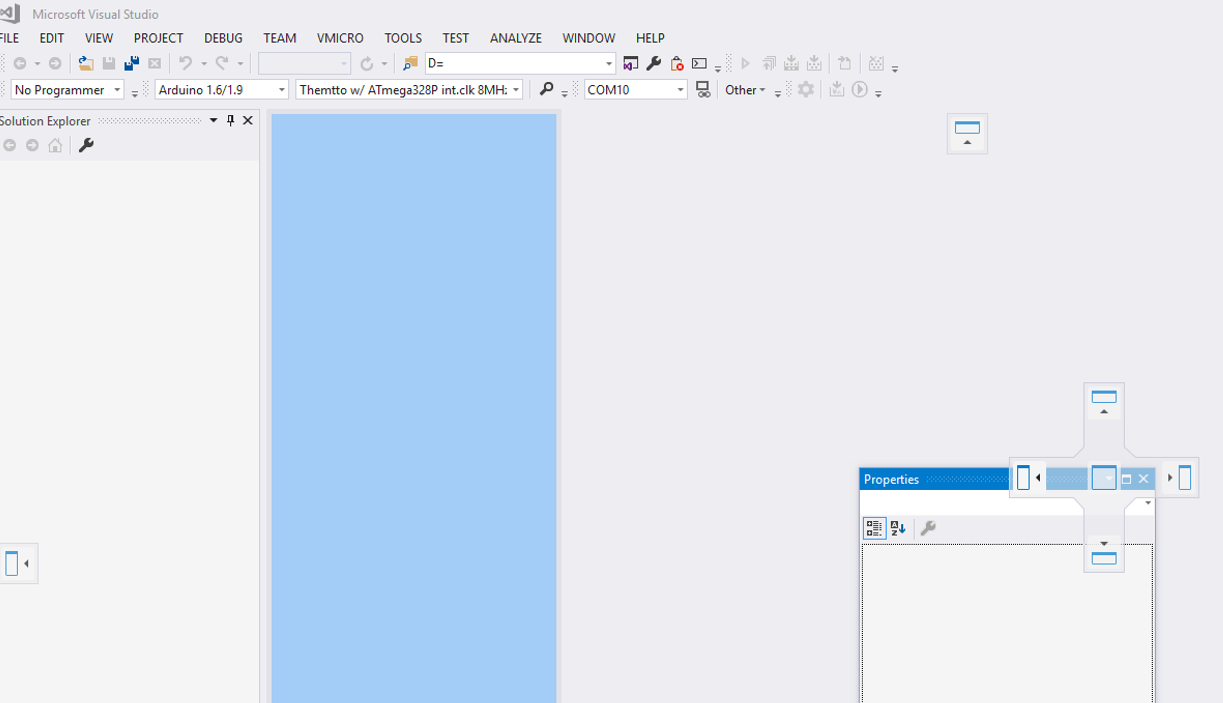
\includegraphics[width= \textwidth]{Figures/Config1}
        \caption{Example of windows distribution with a Fortran project already opened, \textit{Solution Explorer} and \textit{Output} windows are going to be intensively used.}
        \label{fig:Config1}
    \end{figure}

    \newpage
    %%%%%%%%%%%%%%%%%%%%%%%%%%%%%%%%%%%%%%%%%%%%%%%%%%%%%%%%%%%%%%%%%%%%%%%%%%%%%%%%%C
    \item \textbf{Find in Files, Find and Replace} \label{list:FIND}
    
    \textit{Find in Files} is a powerful Visual Studio feature that allows to search in a set of files terms. It can look for the term in the entire solution, only in the opened document, in the opened project, etc. This feature is complemented by the tool \textit{Replace in Files} which can automatically replace all the terms of a project or document by another term. Both tools can be found in the same window: \textit{Find and Replace}. 
    
    Open the window by clicking on \textit{Edit/Find and Replace/Find in Files}, it will be shown at the right part of the IDE by default. Then you can change the position of the window, hide it temporally (with the option of showing it quickly), make it floating or close it, all can be done with the symbols in the top-right part of the window. Once you have the tool opened, change between both features and write a term to look for or replace. The results of the search will appear in the \textit{Find Results} window, which is automatically opened, then it is possible to navigate through the different results in the code itself by pressing \textit{Find previous} and \textit{Find Next}. 
    
    It is a commonly used feature in the IDE so we recommend to maintain the window accessible in the environment. It is treated how to show new commands and toolbars in the section \ref{sec:Shortcuts}. Take a look at the Figure \ref{fig:Config4-2} and check the symbol of the tool \textit{Find in Files}. In addition, \textit{Go To Find Combo} bar is shown in the same toolbar and both icons have to be activated since they are not shown by default.
  

\end{enumerate}


    \vspace{-0.5cm}
    \FloatBarrier
    \section{Importing the environment configuration}
    
This manual is accompanied by a settings file called \texttt{Exported-2019-07-03.vssettings} (or updated name) which makes automatically all the changes explained in this guide. Open this url to download the file:

\url{https://github.com/jahrWork/Visual-Studio-projects}
 
We can import this configuration and then all the options treated will be automatically applied. Go to \textit{Tools/Import and Export Settings/Import selected environment settings} and click on \textit{Next}, in the next window decide if creating or not a backup of your actual configuration, depending on your needs. Click on \textit{Next} again and then in \textit{Browse}, look for the file downloaded from the Git repository and open it. Finally click on \textit{Next} and \textit{Finish}.    
    
If you change the configuration of the environment it is interesting to make a \textbf{backup copy} of the configuration in order to restore it easily if you reinstall Visual Studio, work in two different computers or change your personal computer. Go to \textit{Tools/Import and Export Settings/Export selected environment settings}, click on \textit{Next} twice and choose where to save it.
    
\begin{IN}
    \begin{itemize}
        \item Please notice that the file \texttt{Exported-2019-07-03.vssettings} (or similar name) that comes with this manual only stores the \textbf{IDE configuration} and not the preferences and options related to the project configurations of the different programming languages.
            
        \item It is also important to notice that the configuration file could keep \textbf{sensitive information}, which means that maybe some options store links to folders in the computer where the configuration was made and exported. In this case, when the IDE follows the links an error message appears and you must change the link to the corresponding folder in your computer. This can also happen when you create your own configuration files and use it in more than one computer.  
    \end{itemize}
\end{IN}
    

    \section{Modifying shortcut icons} \label{sec:Shortcuts}

The Figure \ref{fig:Commands} shows some commands that are going to be highly used when programming so we recommend to enable the quick access in the toolbars. The first two of them comment and uncomment the code selected and next two decrease and increase the indentation. The fifth one is the \textit{Start without Debugging} button (already explained) and the last active buttons are in charge of compiling and building our program. While the first compiles the current file, the second builds the project or library selected and the last builds the whole solution (which we know can contain more than one project). These functionalities will be explained in the chapters of the different programming languages. 

\begin{figure}[h]
    \centering
    
\includegraphics[width= 0.9 \textwidth]{Figures/Commands}
    \caption{Very useful commands when programming, it is advisable to show them in the toolbars.}
    \label{fig:Commands}
\end{figure}

\vspace{0.5cm}
We can personalise all the \textbf{toolbars} and \textbf{commands} that the IDE shows and it can be done in two ways. Firstly, by clicking on the right part of each toolbar we see the option \textit{Add or Remove Buttons} which deploys a list of default options for that bar (Figure \ref{fig:Config2}). Secondly, we can click on \textit{Tools/Customize} and we access two tabs: \textit{Toolbars} (Figure \ref{fig:Config3}), which can show and hide a big list of toolbars and \textit{Commands} where we can select any of them, add and delete commands and also add new buttons that are not in the bar by default (figures \ref{fig:Config4-2}, \ref{fig:Config4} and \ref{fig:Config4-3}). 

In these mentioned figures we can see that the \textit{Text Editor}, \textit{Standard}, \textit{Build} and \textit{Micro} toolbars are shown. The Figure \ref{fig:Config4-2} shows that \textit{Standard} bar includes new commands like \textit{Find in Files}, \textit{Solution Explorer} and \textit{Properties Window} while \textit{Build} bar (figure \ref{fig:Config4}) includes \textit{Compile} command and the most important; \textbf{\textit{Start without debugging}}.\label{StartwD} It is necessary to have quick access to this command because most of the times we won't use the default debugger and we just want to run the code directly without debugging. Finally, the toolbar \textit{Text Editor} (figure \ref{fig:Config4-3}) is really useful while writing code because of the \textit{Comment} and \textit{Uncomment} commands or the new ones added, \textit{Line Indent} and \textit{Line Unindent}. We should take the time to organize buttons and include those we use more. 

\begin{figure}[h]
    \centering
    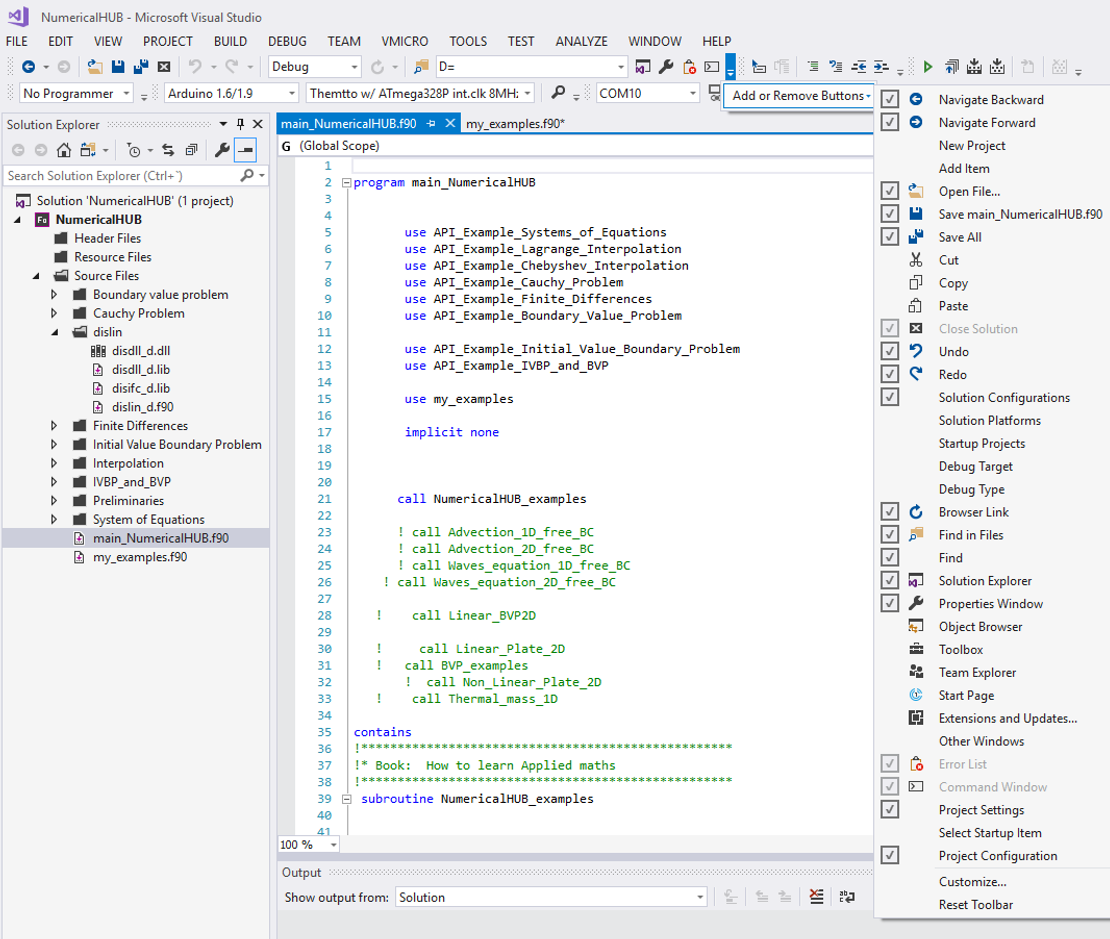
\includegraphics[width=\textwidth]{Figures/Config2}
    \caption{Add and Remove options for the buttons that appear in the toolbars.}
    \label{fig:Config2}
\end{figure}

\begin{figure}[h]
    \centering
    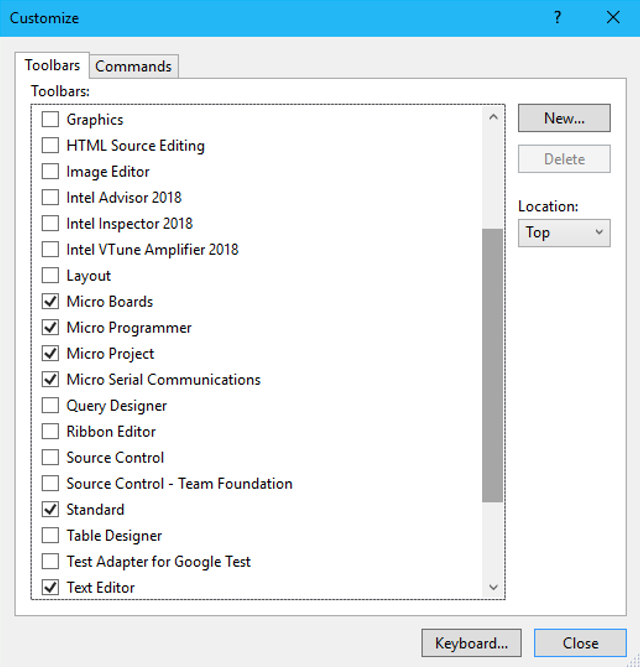
\includegraphics[width= \textwidth]{Figures/Config3}
    \caption{\textit{Toolbars} tab in the menu \textit{Tools/Customize}, it allows to show and hide toolbars for the IDE.}
    \label{fig:Config3}
\end{figure}

\begin{figure}[h]
    \centering
    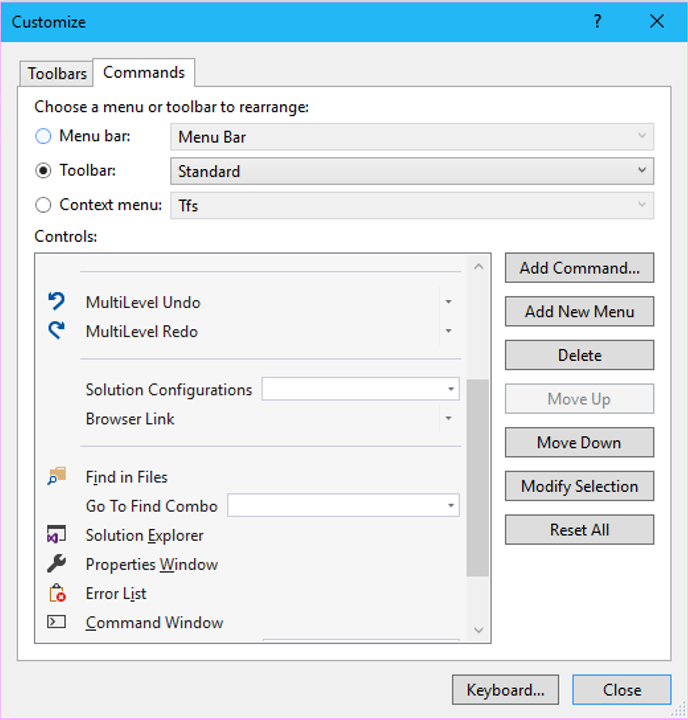
\includegraphics[width= 0.6\textwidth]{Figures/Config4-2}
    \caption{\textit{Commands} tab in the menu \textit{Tools/Customize}, it adds commands to the selected toolbar or menu, in this case the \textit{Standard} Toolbar.}
    \label{fig:Config4-2}
\end{figure}

\begin{figure}[h]
    \centering
    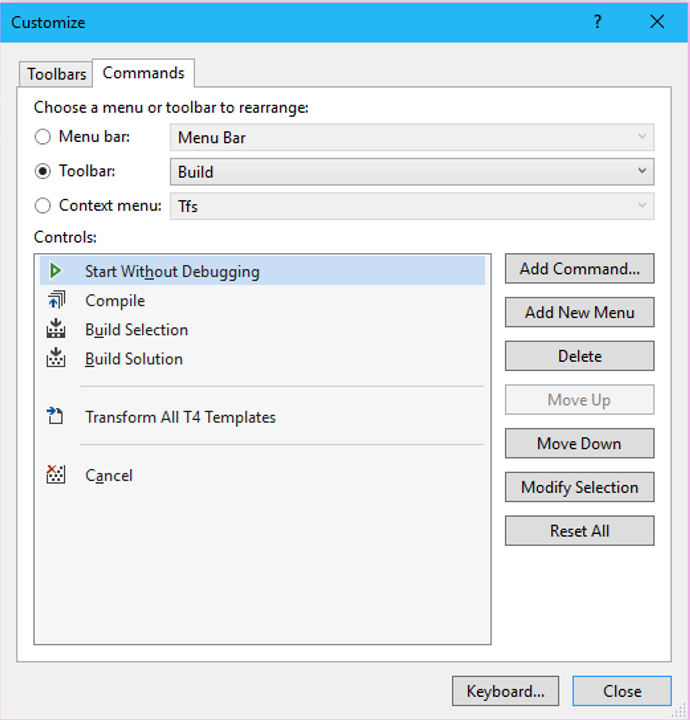
\includegraphics[width= 0.6\textwidth]{Figures/Config4}
    \caption{\textit{Commands} tab in the menu \textit{Tools/Customize}, it adds commands to the selected toolbar or menu, in this case the \textit{Build} Toolbar.}
    \label{fig:Config4}
\end{figure}

\begin{figure}[h]
    \centering
    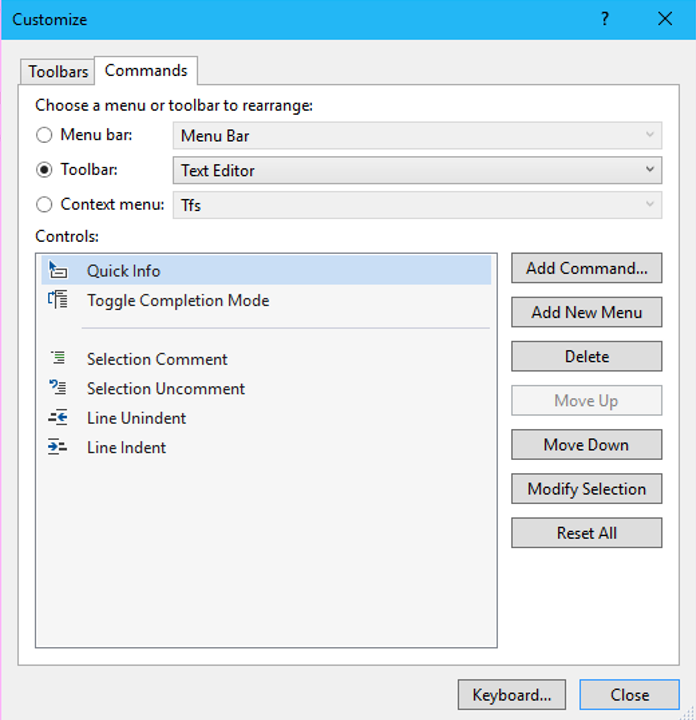
\includegraphics[width= \textwidth]{Figures/Config4-3}
    \caption{\textit{Commands} tab in the menu \textit{Tools/Customize}, it adds commands to the selected toolbar or menu, in this case the \textit{Text Editor} Toolbar.}
    \label{fig:Config4-3}
\end{figure}
    

    
    
    

    \FloatBarrier
    \section{Enterprise distribution of Visual Studio} \label{sec:Enterprise}

If you are interested in the Enterprise distribution of Visual Studio you can download the installer from the same webpage used for the Community version (\url{https://visualstudio.microsoft.com/es/downloads/}) or follow all the steps mentioned below. In this case you need an academic license to activate the product. We are going to see how to obtain that license using \textit{Azure Dev Tools for Teaching}, a Microsoft repository created for university departments and students.

Obtaining an academic license and the installer for Visual Studio Enterprise. 

\begin{enumerate}
    \item Click directly on (Figure \ref{fig:ExtraA}):
    
     \url{https://azureforeducation.microsoft.com/devtools}
    \item Click on the blue button \textit{Sign In} and Initiate session using your institutional email (finished with \textit{@alumnos.upm.es}, Figure \ref{fig:ExtraB}).
    \item You will be redirected to the authentication service of the UPM. Write your email once again and write the password for that email account (Figure \ref{fig:ExtraC}).
    \item After accepting a message that allows you to maintain the session opened, you access the Microsoft Azure environment with the tab \textit{Education} shown (Figure \ref{fig:ExtraD}).
    \item There, you may see the last release of Visual Studio in the right part of the window. However, you can also click on \textit{Software}, look for \textit{Visual Studio Enterprise} in the list or write it in the search bar.
    \item Click on the name of the tool and you will have access to the download of the installer and the Key for activating the product (Figure \ref{fig:ExtraE}). 
    \item Download the installer for the Enterprise distribution and keep safe the Key, you are going to use it later.    
\end{enumerate}

\begin{figure}
    \centering
    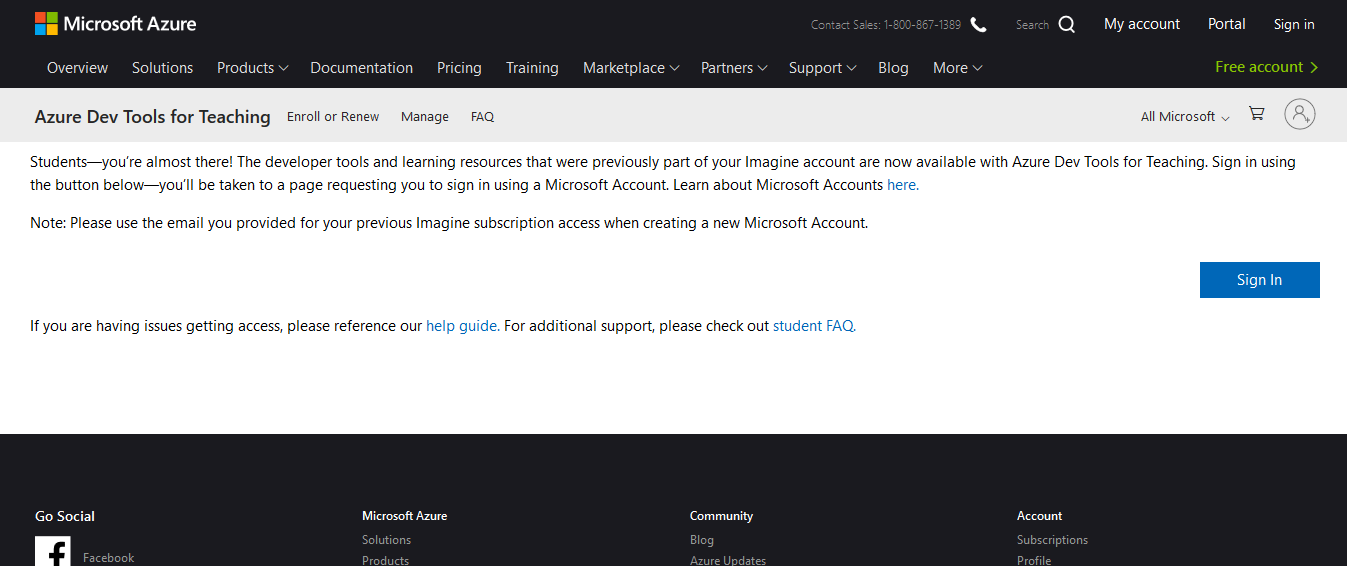
\includegraphics[width= \textwidth]{Figures/ExtraA}
    \caption{Main webpage of Microsoft Azure Dev Tools for Teaching where we have to click on \textit{Sign In}.}
    \label{fig:ExtraA}
\end{figure}

\begin{figure}
    \centering
    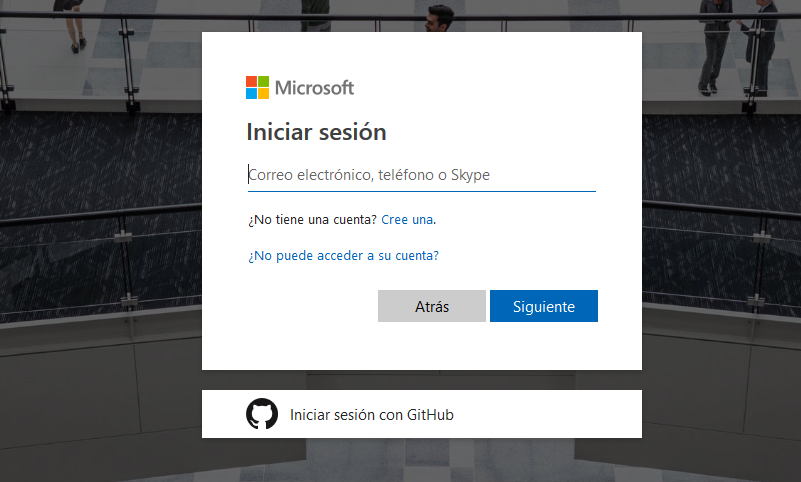
\includegraphics[width= \textwidth]{Figures/ExtraB}
    \caption{Start session window, the institutional email must be used here (finished with @alumnos.upm.es).}
    \label{fig:ExtraB}
\end{figure}

\begin{figure}
    \centering
    
\includegraphics[width= \textwidth]{Figures/ExtraC}
    \caption{Authentication service of the UPM, you must use your institutional email and the same password used in the email account.}
    \label{fig:ExtraC}
\end{figure}

\begin{figure}
    \centering
    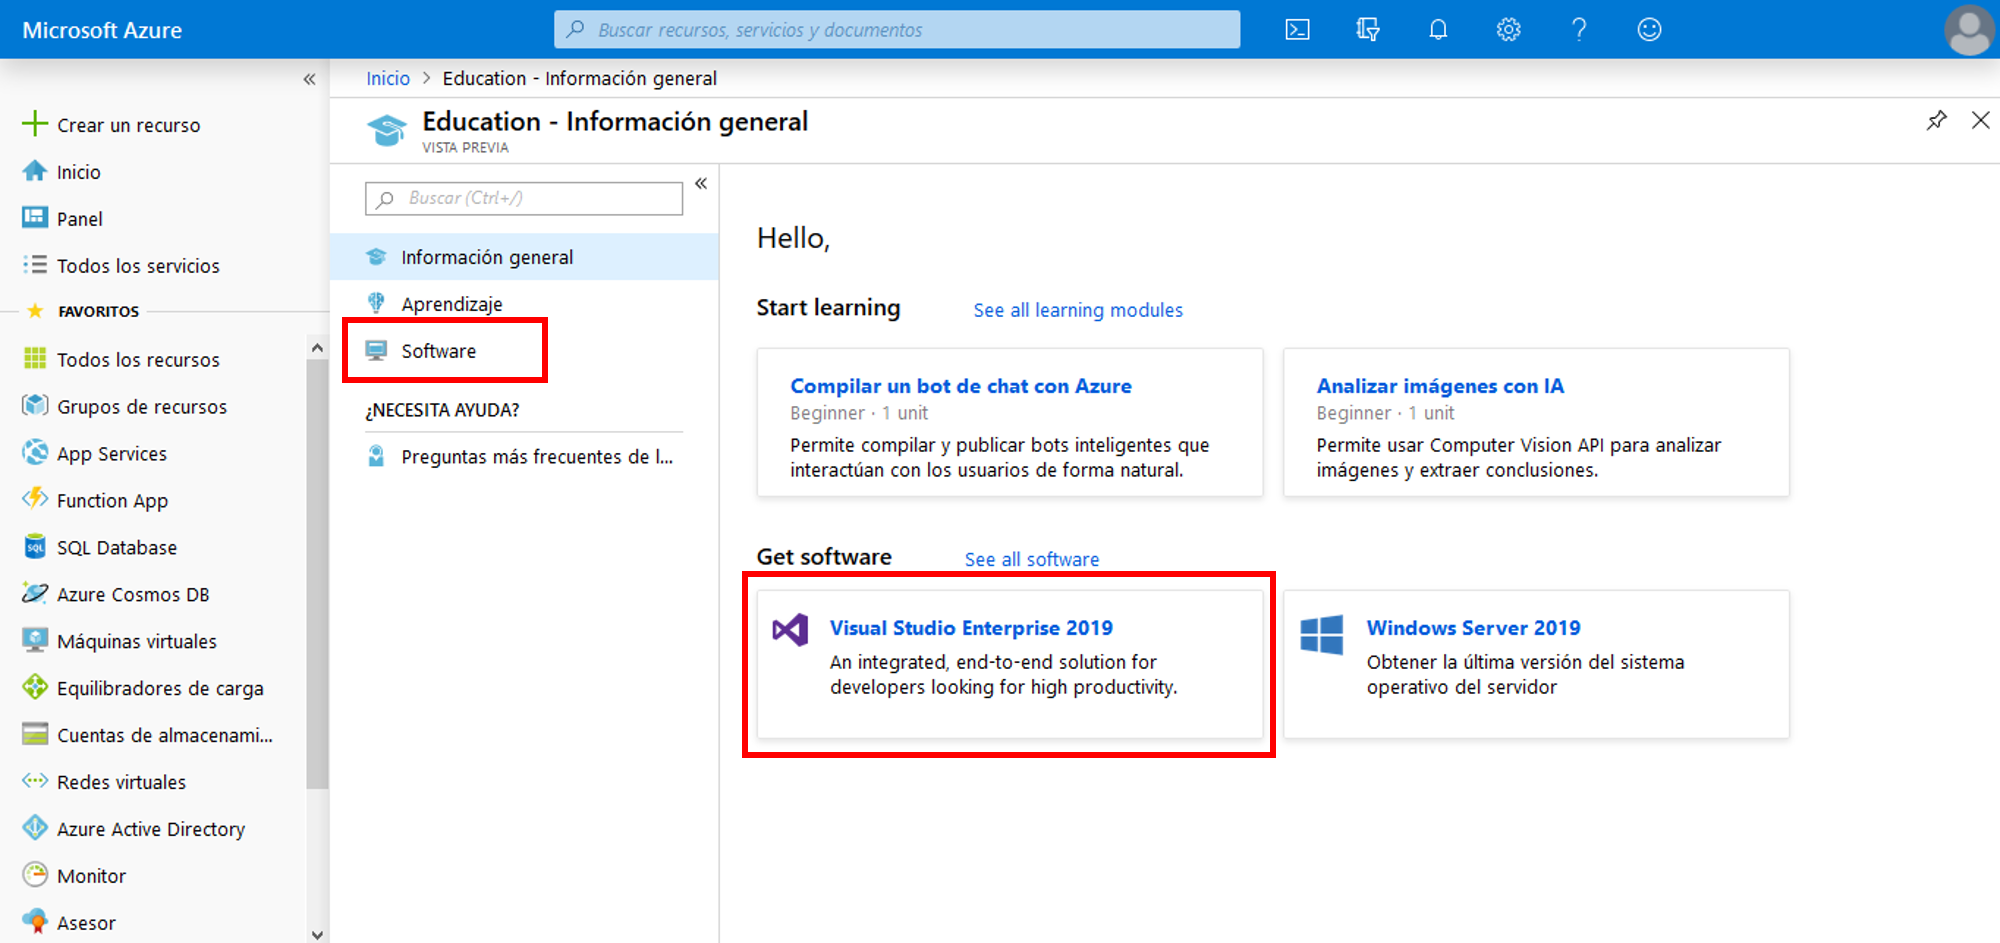
\includegraphics[width= \textwidth]{Figures/ExtraD}
    \caption{Start window of Microsoft Azure, Visual Studio Enterprise is already shown but we could look for it in the \textit{Software} space if needed.}
    \label{fig:ExtraD}
\end{figure}

\begin{figure}
    \centering
    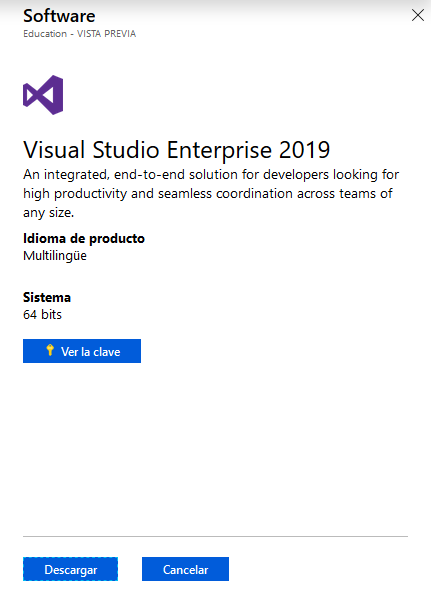
\includegraphics[width= 0.6 \textwidth]{Figures/ExtraE}
    \caption{Menu where we can download the installer of Visual Studio Enterprise and consult the key used to activate the tool.}
    \label{fig:ExtraE}
\end{figure}

In order to install Visual Studio Enterprise version with an academic license in Windows you can follow the same process seen in the installation of the Community version, executing this time the installer of the Enterprise version. The name now is similar to \texttt{vs\_enterprise\_xxxxx.exe}. As a difference, in the step 7 you have to activate the product using your Key:

\begin{enumerate}
    \setcounter{enumi}{6}
    \item Notice that in the top right part of the IDE it is shown that you have already started session. If you click on the letter of your name and \textit{Account Configuration} (see figure \ref{fig:Instalacion3}) you will see that your credentials are activated. In the right part of that window it may say that you are using a 30 days license, click on \textit{Unlock with a Product Key} (see figure \ref{fig:Instalacion5}) and it will show a window waiting for the Key obtained (see figure \ref{fig:Instalacion6}). Click on \textit{Apply} and the message ``Product Key applied'' should appear. 
    \item Your IDE is ready to work now. 
\end{enumerate}

\begin{figure}
    \centering
    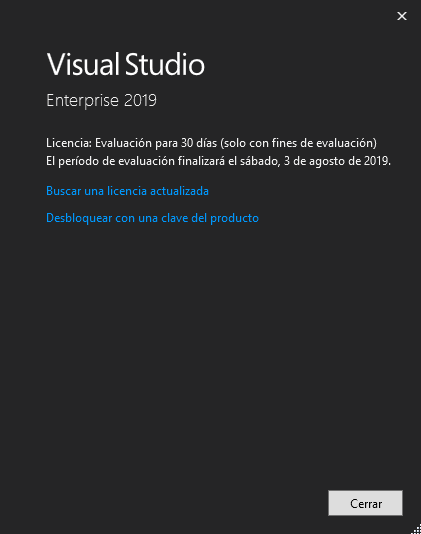
\includegraphics[width= 0.7\textwidth]{Figures/Instalacion5}
    \caption{License information in the Account Configuration window in the IDE, before activating the product you will have a 30 days license.}
    \label{fig:Instalacion5}
\end{figure}

\begin{figure}
    \centering
    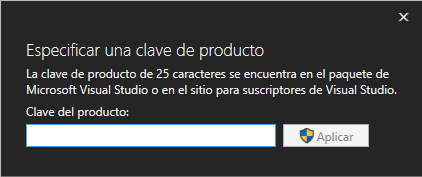
\includegraphics[width= 0.6\textwidth]{Figures/Instalacion6}
    \caption{Activation window, copy here the key obtained with \textit{Azure Dev Tools for Teaching} and click on \textit{Apply}.}
    \label{fig:Instalacion6}
\end{figure}



%------------------------------------------------------------------------------------------------------------------------------------------------------
%------------------------------------------------------------------------------------------------------------------------------------------------------
%As an example, we are going to see how to download Visual Studio with academic license using \textit{OnTheHub}, a repository where essential tools of the industry are offered to the universities.
%
%\begin{enumerate}
%    \item We click directly on this url; \url{http://e5.onthehub.com/WebStore/ProductsByMajorVersionList.aspx?ws=f1b11fc4-826f-e011-971f-0030487d8897&vsro=8&JSEnabled=1}.
%    \item Log in here (top right part of the window) using our institutional email (finished with \textit{@alumnos.upm.es}) and enter with same password as our personal account (figure \ref{fig:Proceso1}).
%    \item In the search line we write ``Visual Studio Enterprise 2017''. The first result that appears is our IDE, we click on \textit{Add to cart} and go to the Shopping Cart.
%    \item Follow the instructions shown. We will be asked for the name, surname and email for confirming the process (Figure \ref{fig:Proceso2} and \ref{fig:Proceso3}).
%    \item Once we complete the information, the details of the purchase appear with the Order Number and the License Key (an email with the purchase details is also sent to our account). Figure \ref{fig:Proceso4} shows the download button. Do not forget to store the License Key and the Order Number for future requests. 
%    \item Click on \textit{Download}. The file \textit{vs\_enterprise\_xxxxx.exe} should be downloaded in your downloads folder.      
%\end{enumerate}
%
%\begin{figure}
%    \centering
%    
\includegraphics[width= \textwidth]{Figures/Proceso1}
%    \caption{Home page of the software repository of Microsoft, we log in and search for Visual Studio 2017.}
%    \label{fig:Proceso1}
%\end{figure}
%
%\begin{figure}
%    \centering
%    
\includegraphics[width= \textwidth]{Figures/Proceso2}
%    \caption{Version of Visual Studio chosen, Enterprise 2017. We have to write name, surname and email.}
%    \label{fig:Proceso2}
%\end{figure}
%
%\begin{figure}
%    \centering
%    
\includegraphics[width= \textwidth]{Figures/Proceso3}
%    \caption{Shopping Cart with Visual Studio Enterprise 2017 chosen.}
%    \label{fig:Proceso3}
%\end{figure}
%
%\begin{figure}
%    \centering
%    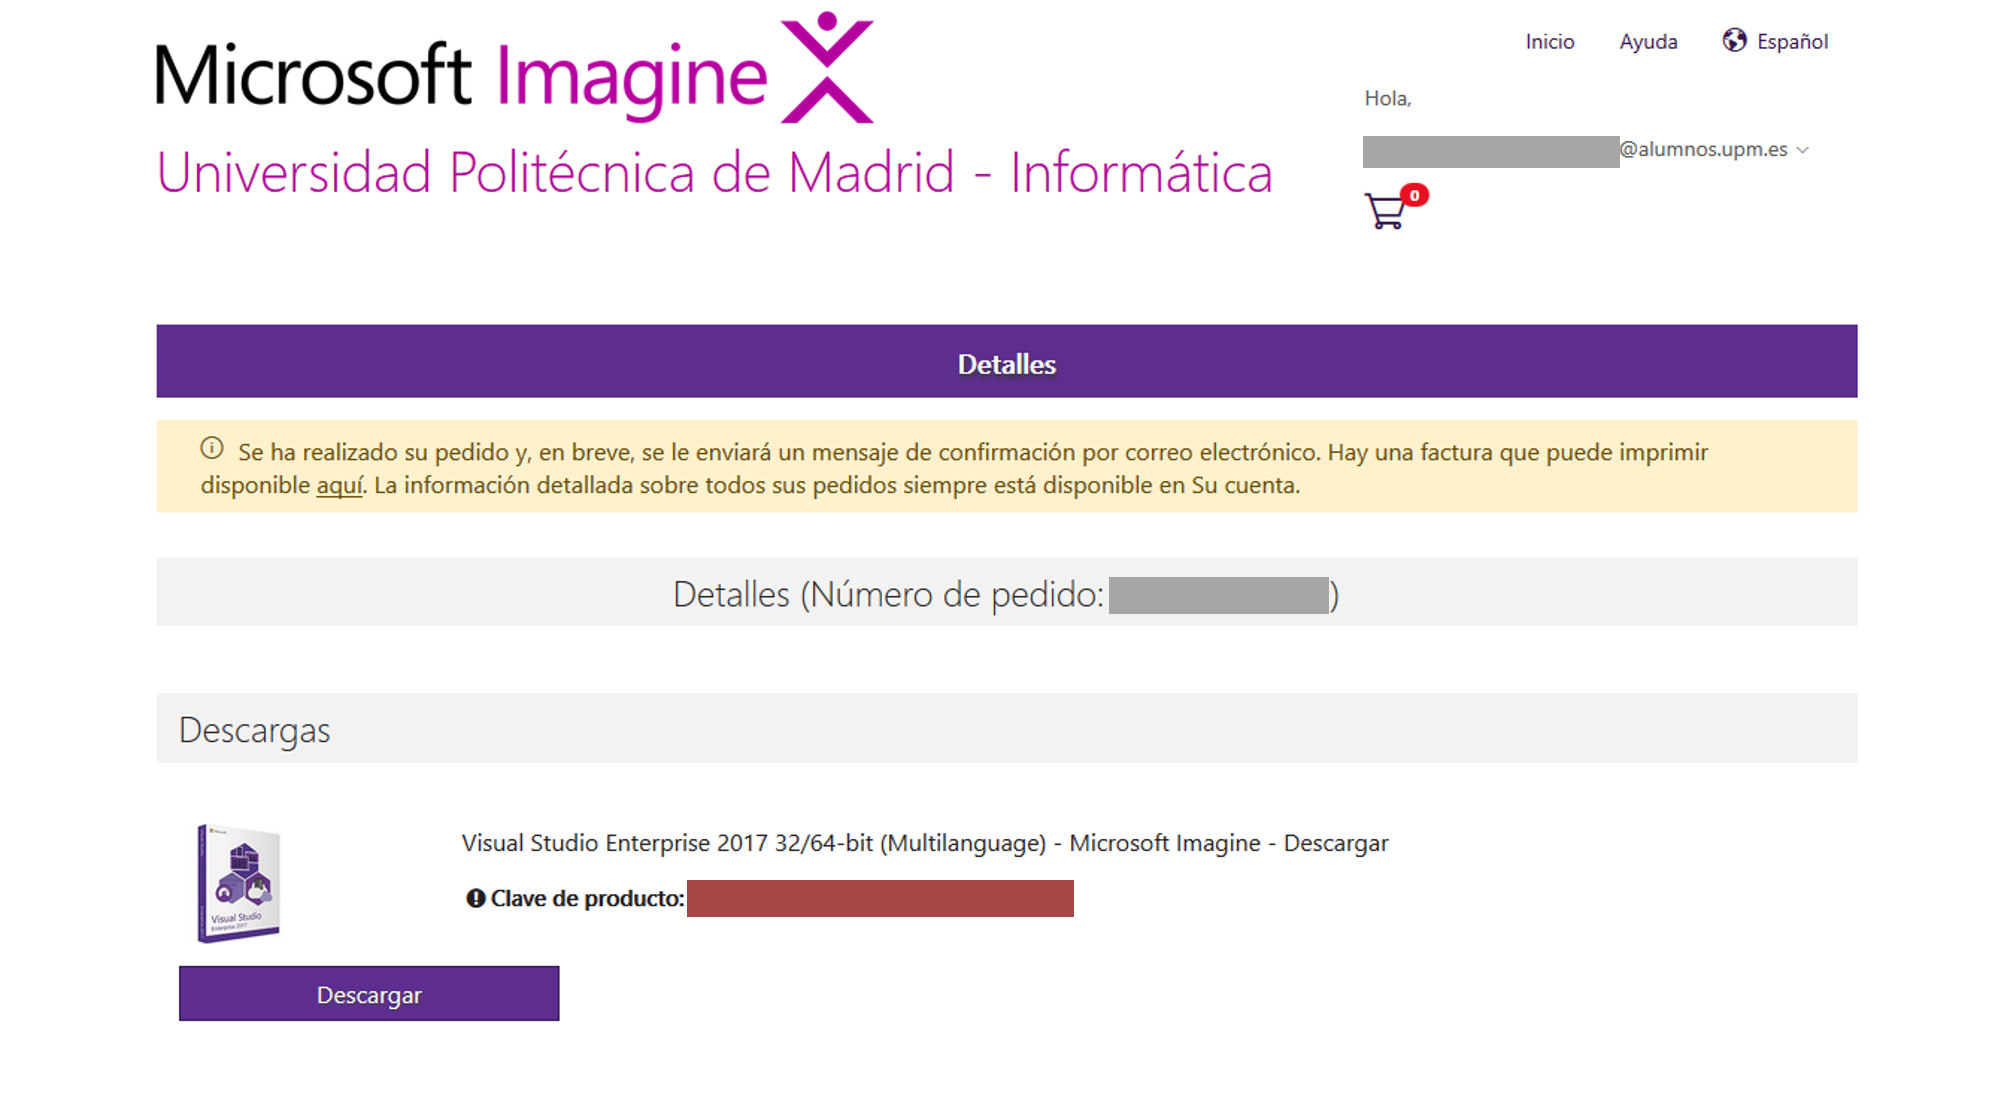
\includegraphics[width=  \textwidth]{Figures/Proceso4}
%    \caption{Details of our License Key and Order Number, we should save this information.}
%    \label{fig:Proceso4}
%\end{figure}
%------------------------------------------------------------------------------------------------------------------------------------------------------
%------------------------------------------------------------------------------------------------------------------------------------------------------



   
    % !TeX spellcheck = en
\chapter{Python Projects} \label{sec:Python}

    \FloatBarrier
    \section{Installing Python Interpreter}

Visual Studio supports Python projects and solutions by selecting during the Visual Studio installation the \textbf{Python Development} workload. If we do not have installed it yet, we can always do it when needed thanks to the Visual Studio Installer tool. In order to do that:

\begin{enumerate}
	\item Open \textit{Visual Studio Installer} application as an administrator.
	%\item It may happen that the program requires an upgrade. Click on \textit{Update} and wait for the installation to finish.
	\item Click on \textit{Modify} on the space reserved for your currently version of Visual Studio (Figure \ref{fig:vsi:list}). %If the \textit{Update} button were to appear instead, click on \textit{Update} and wait for the installation to complete, the \textit{Modify} button should be now available.
	\item Now, in the \textit{Workloads} tab, select \textit{Python Development}. Check that the first three elements of the optional modules to be installed are selected (\texttt{Python 3 xx-bit (3.x.x)} included), it can be checked on the right part of the window as it is shown in the Figure \ref{fig:vsi:mods}.
	\item Click on \textit{Modify} and wait until the installation has finished.
\end{enumerate} 

%After installation has finished Python projects can be created and configured at the IDE.

\begin{figure}
	\centering
	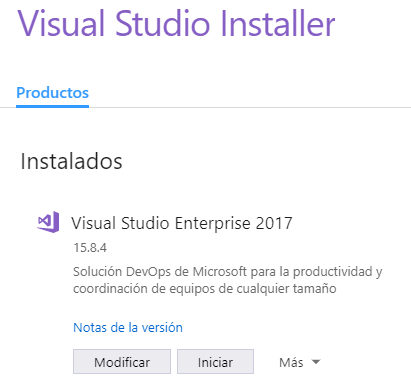
\includegraphics[scale=0.65]{./Figures/PT0.png}
	\caption{Main window of the Visual Studio Installer with the release Enterprise 2017 shown.}
	\label{fig:vsi:list}
\end{figure}

\begin{figure}
	\centering
	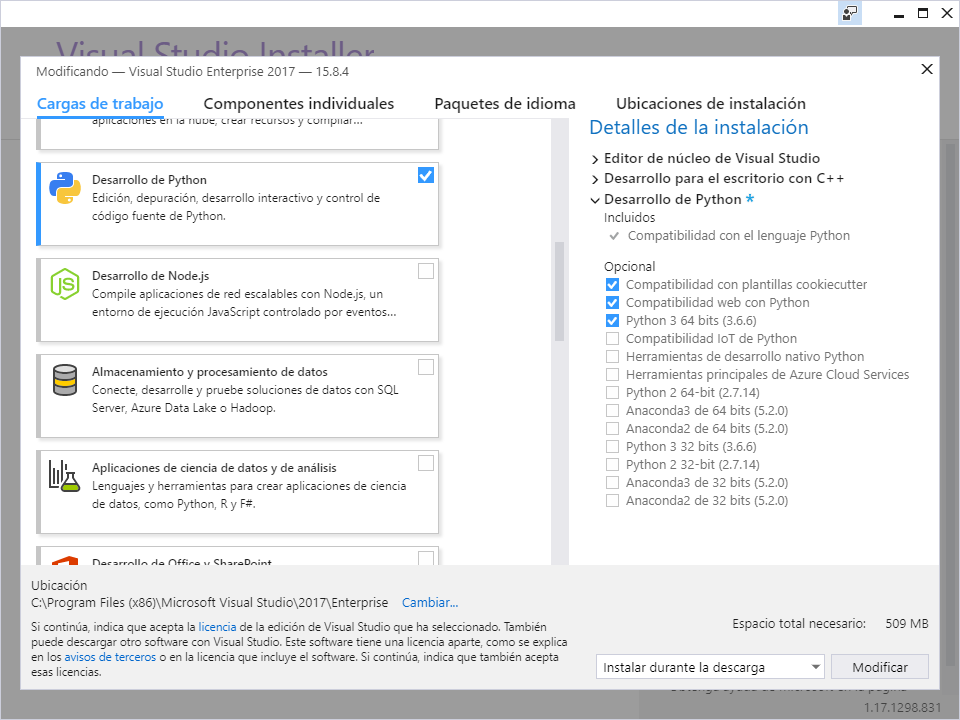
\includegraphics[scale=0.5]{./Figures/PT1V2.png}
	\caption{Workloads ready to be installed using the Visual Studio Installer. The Python development is already selected and the needed characteristics chosen.}
	\label{fig:vsi:mods}
\end{figure}


%This chapter consists of a several steps in order to get embedded Python 
%Project support.
%\begin{enumerate}
%\item Create a new project.
%
%On the top-left corner, check the option 
%\textbf{``FILE{$\rightarrow$}New{$\rightarrow$}Project...''}.
%\item Browse Python templates.
%
%On the newly opened window's left panel, expand the following arrow tree: 
%\textbf{``Installed{$\rightarrow$}Templates{$\rightarrow$}Python''}.
%
%
%
%\item Download additional Python Software.
%
%Hit on \textbf{``Get Python Tools for Visual Studio''} and click on \textbf{OK}.
%\ref{fig:PyStep1}
%%1
%
%
%A new tab will pop-up. Click on \textbf{``Download Python Tools for Visual 
%Studio''}.
%\ref{fig:PyStep2}
%%2
%
%\item Install additional Python Software.
%
%Upon finishing the download an installation will request Administrator 
%permissions, grant them by clicking on \textbf{``Execute''}.
%\ref{fig:PyStep34}
%%34
%
%During the installation wizard the user must accept the License Agreement terms 
%as well as close all Visual Studio running windows.
%
%To finish the installation, click on \textbf{``Finish''}. Run Visual Studio 
%again.
%\ref{fig:PyStep567}
%%567
%
%\item Create a new Python project.
%
%On the top-left corner, go to 
%\textbf{``FILE{$\rightarrow$}New{$\rightarrow$}Project...''} and start a any 
%Python project template on 
%\textbf{Installed{$\rightarrow$}Templates{$\rightarrow$}Python}.
%
%\ref{fig:PyStep8}
%%8
%
%\end{enumerate}
%
%
%\begin{figure}[h]
%    \centering
%    \caption{Selecting new Python Project without Python Tools.}
%    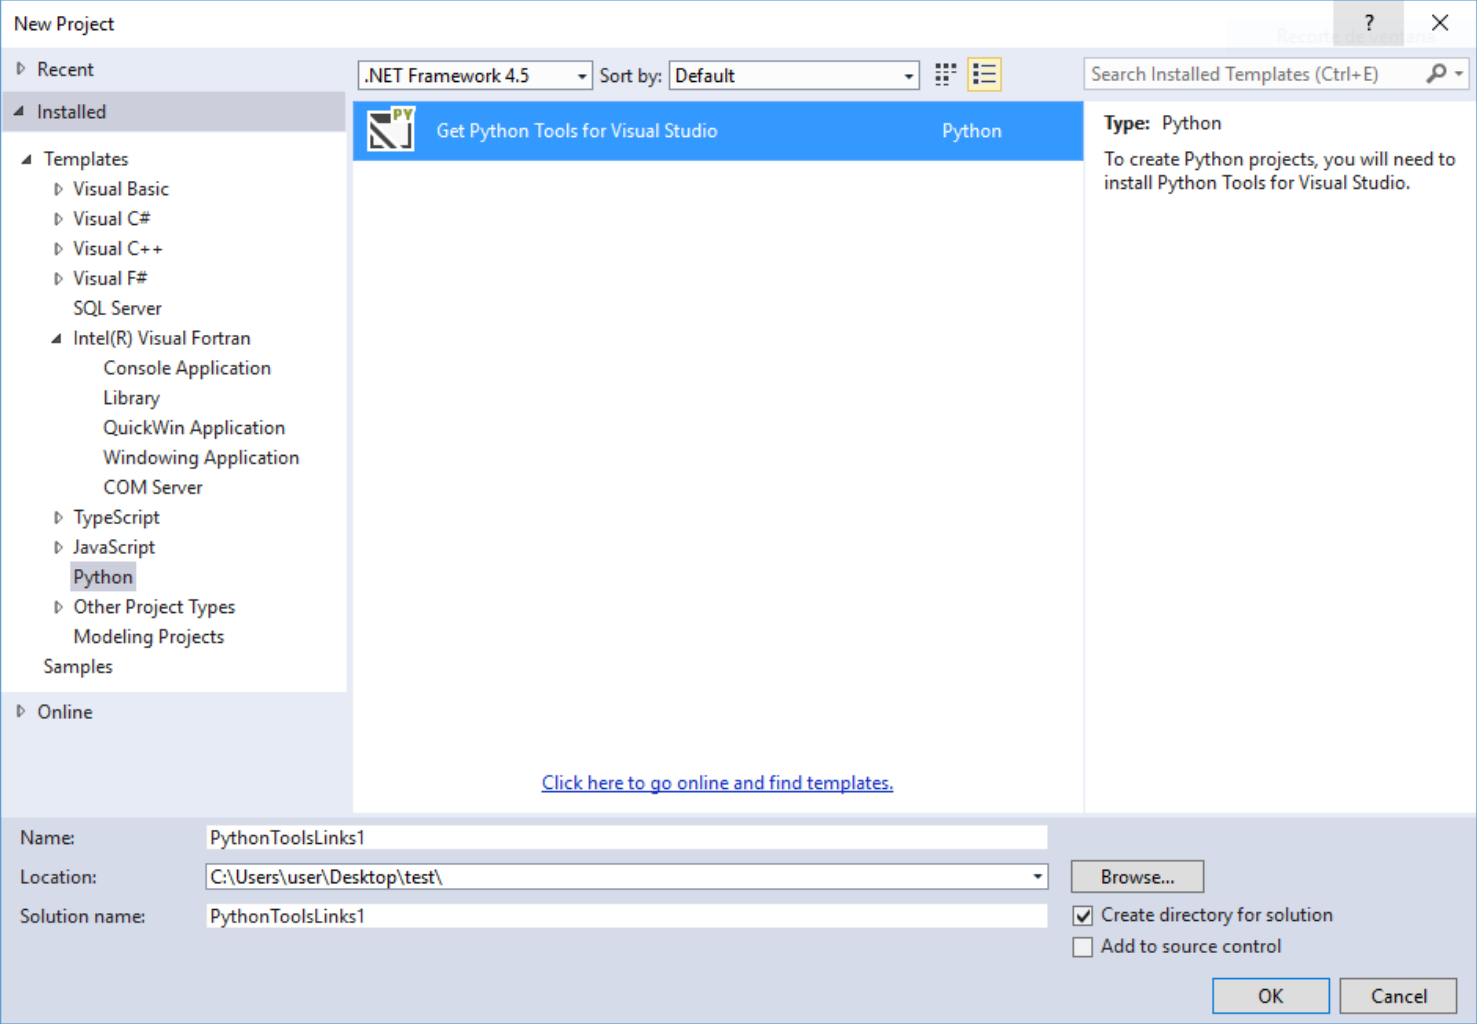
\includegraphics[width= 0.85 \textwidth]{Figures/step1v2.png}
%    \label{fig:PyStep1}
%\end{figure}
%
%
%\begin{figure}[h]
%    \centering
%    \caption{Visual Studio link to Python Tools Installer.}
%    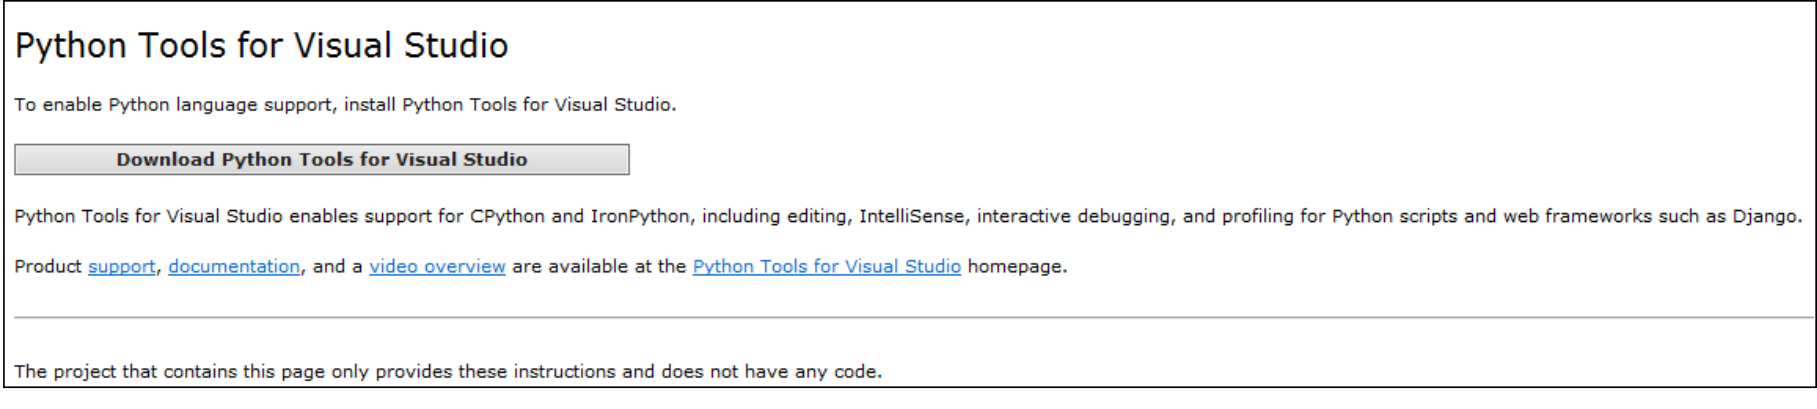
\includegraphics[width= 0.85 \textwidth]{Figures/step2v2.png}
%    \label{fig:PyStep2}
%\end{figure}
%
%\begin{figure}[h]
%\centering
%\caption{Python Tools Programs to be installed.}
%\begin{subfigure}[t]{.5\linewidth}
%\centering
%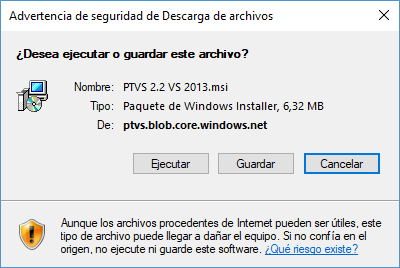
\includegraphics[width= 0.85 \textwidth]{Figures/step3.png}
%\end{subfigure}%
%\begin{subfigure}[t]{.5\linewidth}
%\centering
%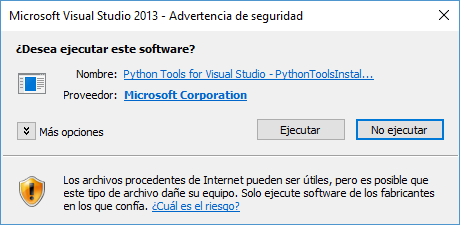
\includegraphics[width= 0.85 \textwidth]{Figures/step4.png}
%\end{subfigure}\\[1ex]
%\label{fig:PyStep34}
%\end{figure}
%
%\begin{figure}[h]
%\caption{Input and warnings from the Installation Setups.}
%\begin{subfigure}{.5\linewidth}
%\centering
%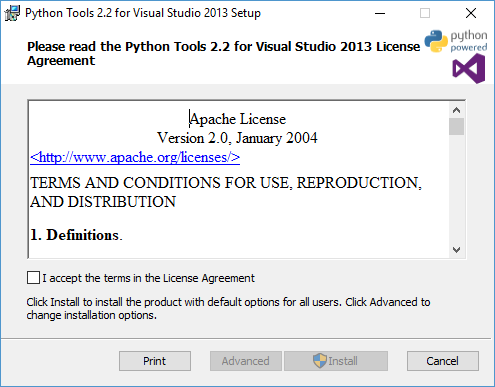
\includegraphics[width= 0.85 \textwidth]{Figures/step5.png}
%\end{subfigure}%
%\begin{subfigure}{.5\linewidth}
%\centering
%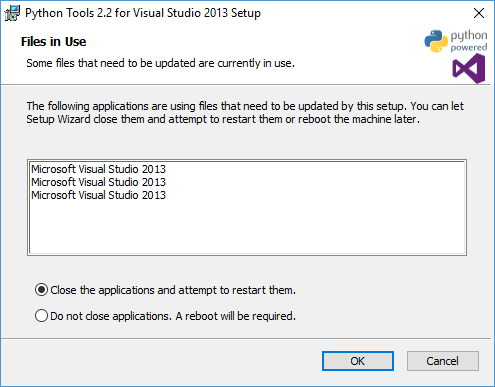
\includegraphics[width= 0.85 \textwidth]{Figures/step6.png}
%\end{subfigure}\\[4ex]
%\begin{subfigure}{\linewidth}
%\centering
%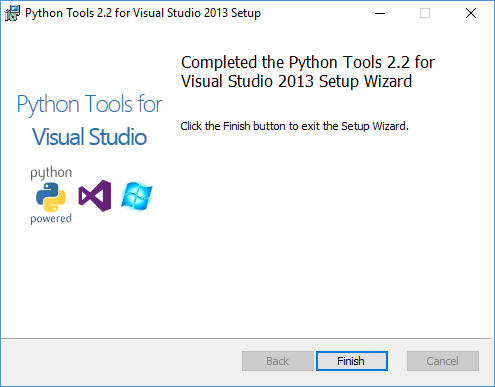
\includegraphics[width= 0.85 \textwidth]{Figures/step7.png}
%\end{subfigure}
%\label{fig:PyStep567}
%\end{figure}
%
%\begin{figure}
%\centering
%\caption{Selecting new Python Project with Python Tools.}
%\begin{normalsize}
%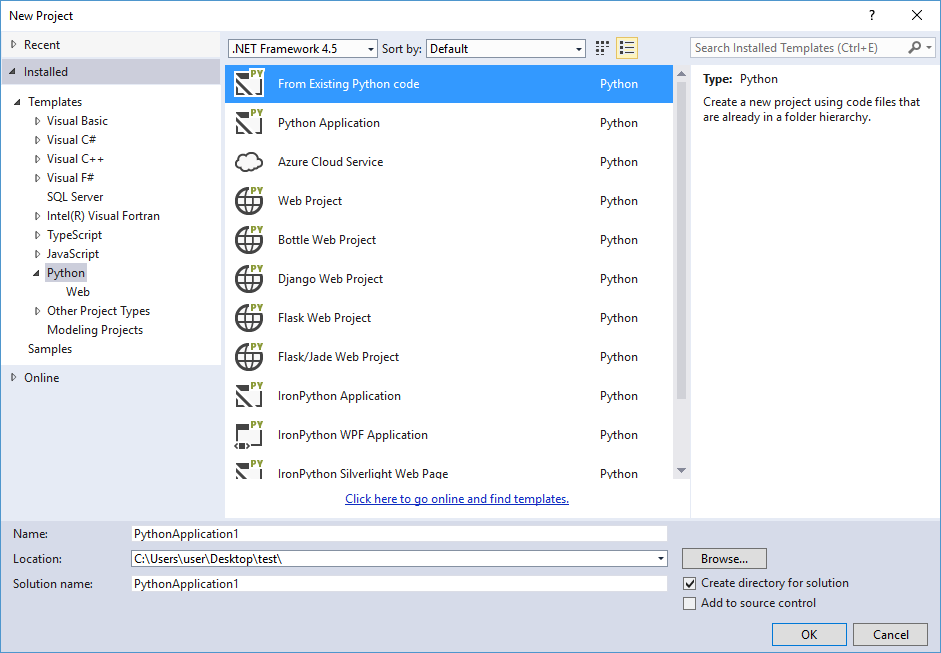
\includegraphics[width= 0.85 \textwidth]{Figures/step8.png}
%\end{normalsize}
%\label{fig:PyStep8}
%\end{figure}
%\clearpage


    
    \section{Create a Python project}

We will see during this guide that the process for creating a new project is similar for all the programming languages, in the case of a Python project:

\begin{enumerate}
	\item Open your version of Visual Studio.
	\item Click on \textit{File/New/Project...}
	\item In the \textit{Python} menu select \textit{Python Application}.
	\item Choose a name for the project (Figure \ref{fig:PP0}).
    \item Change the \textit{Location} of the solution, a directory will be created there.
	\item Select option \textit{Create directory for solution}.
	\item Choose the name of the solution, it does not have to be the same as the name of the project.	
	\item Click on \textit{OK}.
\end{enumerate}

\begin{figure}[h]
    \centering
    \includegraphics[width= \textwidth]{Figures/PP0V2.png}
    \caption{Window \textit{New Project} where creating a Python project.}
    \label{fig:PP0}
\end{figure}



    \section{Execute the ``Hello World'' example}

This first example ensures that the installation has finished correctly. Like in the rest of the programming languages, it writes a ``Hello World'' message on the console. In this case, there is not a template already written with this example so we will write it from scratch. Open the project created in the previous section, you will find a \texttt{.py} file with the same name as the project, open it and write the following code: %\vskip \baselineskip

\vspace{0.5cm} 
\begin{lstlisting}
     print("Hello World!")
\end{lstlisting}

Now, in order to execute this Python script, the interpreter has to be called for translating it to machine code dynamically:

\begin{enumerate}
	\item Click on \textit{DEBUG/Start Without Debugging} or click on the corresponding icon. The program is then executed on a new command prompt.
\end{enumerate}

\begin{IN}
    More project/solution examples with Python language can be downloaded from:
    
     \url{https://github.com/jahrWork/Visual-Studio-projects}.
\end{IN}

    \section{Installing and removing Python Packages}

Python can download projects developed by other people and include them in our own solutions. These projects or \textbf{packages} have been tested by experts to ensure a proper performance and can help us while coding with no need of developing the code from scratch. In order to install a package follow the next steps:

\newpage
\begin{enumerate}[nosep]
	\item Open your Python Project.
	\item If the Solution Explorer is not opened, click on \textit{View/Solution Explorer}.
	\item Unfold the \textit{Python Environments} menu inside the directory of the specific project in the solution explorer.
	\item Right click on \texttt{Python x.x (xx-bit)} and select \textit{Install Python package...} (Figure \ref{fig:pkg0}).
	\item Type the \textit{Package name} to be installed and press on \textit{Enter} (Figure \ref{fig:pkg1}).
	\item A new window will ask you for \textbf{Administrator privileges} as shown on Figure \ref{fig:pkg15}. Select the third option: \textit{Always elevate when installing or removing packages} and Visual Studio will grant permissions automatically.
    \item The process of downloading and installing starts.
	%\item On the \textit{Solution Explorer} tab on \textit{Solution 
	%%%name/Python Environments/Python x.x (xx-bit)} menu and check if the 
	%%%%\textbf{package} appears ().
\end{enumerate}

\begin{figure}[h]
    \centering
    \includegraphics[width= 0.9 \textwidth]{Figures/PPM0V1.png}
    \caption{First step to install new Python packages on the Python environment.}
    \label{fig:pkg0}
\end{figure}

\begin{figure}[h]
    \centering
    \includegraphics[width=0.6 \textwidth]{Figures/PPM1V2.png}
    \caption{Second step to install new Python packages on the python environment. Write here the name of the package to be installed.}
    \label{fig:pkg1}
\end{figure}

\begin{figure}[h]
	\centering
	\includegraphics[width=0.6 \textwidth]{Figures/PPM15.png}
	\caption{Confirmation of the administrator privileges in order to install or remove packages. Click on \textit{Always elevate when installing or removing packages}.}
	\label{fig:pkg15}
\end{figure}

\newpage
If a package is not needed anymore, it can be removed from the environment by following the next steps:

\begin{enumerate}
	\item Open a Python Project.
	\item Unfold the \textit{Python Environments/Python x.x (xx-bit)} menu in the Solution Explorer.
	\item Right click on the \textit{Package name} to be removed and select \textit{Remove} (Figure \ref{fig:pkg2}). 
\end{enumerate}

\begin{figure}[h]
    \centering
    \includegraphics[width= 0.9 \textwidth]{Figures/PPM2V1.png}
    \caption{Option reserved for removing those Python packages not needed from the Python environment.}
    \label{fig:pkg2}
\end{figure}

%\section{Configuring a Python Environment}
%
%In previous sections we've seen how to create Python projects with the default configuration of VS. As opposed to Fortran projects where a unique compiler makes use of selected source files, Python projects execute an script and the required source files with a configurable \textbf{Python Environment}. This environment is composed by the \textbf{Python Interpreter}, which specifies the programming language version (2.7, 3.5, 3.6, etc.), and the \textbf{installed packages} from other sources.
%
%On the \textbf{``Solution Explorer''} panel, check whether the \textbf{``Python 
%Environment''} option is expandable and contains a suitable environment.
%
%If affirmative, no more further steps are required, else continue to the 
%following step.
%
%\begin{enumerate}
%
%\item Right-click on \textbf{``Python Environment''} and select 
%\textbf{``Add/Remove Python Environments''}.
%\ref{fig:PyStep9}
%%9
%
%\begin{figure}[h]
%\centering
%\caption{Add a new Environment.}
%\includegraphics[width=0.85 \textwidth]{Figures/step9v2.png}
%\label{fig:PyStep9}
%\end{figure}
%
%\item Select an environment of your choice if any, and click on \textbf{``OK''}.
%\ref{fig:PyStep10}
%%10
%
%\begin{figure}[h]
%\centering
%\caption{Available Python Environments}
%\includegraphics[width=0.85 \textwidth]{Figures/step10.png}
%\label{fig:PyStep10}
%\end{figure}
%
%\end{enumerate}
%
%\section{Configure a custom Python Environment}
%
%It may happen that no environment has been detected or that the selected one 
%does not work (a warning icon is displayed next to it). In these cases a custom 
%configuration is needed.
%
%\begin{enumerate}
%
%\item Open the \textbf{``Python Environments''} panel by clicking on 
%\textbf{``VIEW{$\rightarrow$}Other Windows{$\rightarrow$}Python Environments''}.
%
%\item Select \textbf{``Custom...''}. Configure all the fields with your custom 
%installation. Click on \textbf{Apply} to save the changes. 
%\ref{fig:PyStep11}
%%11
%
%\begin{figure}[h]
%\centering
%\caption{Custom Python Environment installed on shared partition.}
%\includegraphics[width=0.75 \textwidth]{Figures/step11v2.png}
%\label{fig:PyStep11}
%\end{figure}
%
%\item On the \textbf{``Solution Explorer''} panel,right-click on 
%\textbf{``Python Environment''} and select \textbf{``Add/Remove Python 
%Environments''}. Select the newly created environment and hit the \textbf{OK} 
%button.
%\ref{fig:PyStep12}
%%12
%
%\begin{figure}[h]
%\centering
%\caption{New custom Python Environments available.}
%\includegraphics[width=0.85 \textwidth]{Figures/step12.png}
%\label{fig:PyStep12}
%\end{figure}
%
%\end{enumerate}
%
%%---------


%Sometimes due to Visual Studio not finding a suitable Python installation it is 
%necessary to edit the default configuration.
%
%The malfunctioning tents to happen with custom Python installations on 
%non-regular directories or Visual Studio selecting partially removed previous 
%working folders.
%
%If your project does not run properly when hitting the \textbf{``Start''} 
%button you must consider following this chapter's instructions.

%\section{Select a Python Environment}
%
%A Python Environment consists of the following elements.
%\begin{itemize}
%\item A python compiler \textbf{python(.exe)}, version 2.X or 3.X. Executes 
%python scripts.
%\item A python windowed interpreter \textbf{pythonw(.exe)}, which executes 
%commands written on a terminal.
%\item A python \textbf{library folder} where modules and package manager such 
%as \textit{pip} or \textit{easy\_install} are located.
%\end{itemize}
%
%All the elements must be located and correctly bound to the Operating System's 
%programs and libraries. This means that copy-pasting a certain module folder to 
%another environment will not work.
%
%On the \textbf{``Solution Explorer''} panel, check whether the \textbf{``Python 
%Environment''} option is expandable and contains a suitable environment.
%
%If affirmative, no more further steps are required, else continue to the 
%following step.
%
%\begin{enumerate}
%
%\item Right-click on \textbf{``Python Environment''} and select 
%\textbf{``Add/Remove Python Environments''}.
%\ref{fig:PyStep9}
%%9
%
%\begin{figure}[h]
%\centering
%\caption{Add a new Environment.}
%\includegraphics[width=0.85 \textwidth]{Figures/step9v2.png}
%\label{fig:PyStep9}
%\end{figure}
%
%\item Select an environment of your choice if any, and click on \textbf{``OK''}.
%\ref{fig:PyStep10}
%%10
%
%\begin{figure}[h]
%\centering
%\caption{Available Python Environments}
%\includegraphics[width=0.85 \textwidth]{Figures/step10.png}
%\label{fig:PyStep10}
%\end{figure}
%
%\end{enumerate}
%
%\section{Configure a custom Python Environment}
%
%It may happen that no environment has been detected or that the selected one 
%does not work (a warning icon is displayed next to it). In these cases a custom 
%configuration is needed.
%
%\begin{enumerate}
%
%\item Open the \textbf{``Python Environments''} panel by clicking on 
%\textbf{``VIEW{$\rightarrow$}Other Windows{$\rightarrow$}Python Environments''}.
%
%\item Select \textbf{``Custom...''}. Configure all the fields with your custom 
%installation. Click on \textbf{Apply} to save the changes. 
%\ref{fig:PyStep11}
%%11
%
%\begin{figure}[h]
%\centering
%\caption{Custom Python Environment installed on shared partition.}
%\includegraphics[width=0.75 \textwidth]{Figures/step11v2.png}
%\label{fig:PyStep11}
%\end{figure}
%
%\item On the \textbf{``Solution Explorer''} panel,right-click on 
%\textbf{``Python Environment''} and select \textbf{``Add/Remove Python 
%Environments''}. Select the newly created environment and hit the \textbf{OK} 
%button.
%\ref{fig:PyStep12}
%%12
%
%\begin{figure}[h]
%\centering
%\caption{New custom Python Environments available.}
%\includegraphics[width=0.85 \textwidth]{Figures/step12.png}
%\label{fig:PyStep12}
%\end{figure}
%
%\end{enumerate}

    \section{Include modules \& packages from other Projects}

Python Projects can ``import'' modules and packages from other projects on separated directories. With this way we can have the latest updates of an actively developed module or package without duplicating code. There are two ways for including external modules and packages:

\subsection*{Modules/Packages from the same solution}

\begin{itemize}
	\item In the solution explorer, in a project, right click on \textit{References} and select \textit{Add Reference...}
	\item Check Python Projects in order to import their modules and packages as shown on Figure \ref{fig:refs0}.
\end{itemize}

\begin{figure}[h]
    \centering
    \includegraphics[width= \textwidth]{Figures/PPR0.png}
    \caption{Available Python Projects for importing packages. Each project contains a package with the same name on its root directory.}
    \label{fig:refs0}
\end{figure}

\subsection*{Modules/Packages outside solution}

\begin{itemize}
	\item In the solution explorer, in a project, right click on \textit{Search Paths} and select \textit{Add Folder to Search Path...}
	\item Select the root folder where the Python module/package to be imported is located (see Figure \ref{fig:refs1}).
\end{itemize}

\begin{figure}[h]
    \centering
    \includegraphics[width=\textwidth]{Figures/PPR1.png}
    \caption{In this window we can look for the path of the package to be used by the Python Project.}
    \label{fig:refs1}
\end{figure}

   
    \chapter{Arduino Projects}

    \section{Install Visual Micro plug--in}
    
Visual Micro is a plug--in for Microsoft Visual Studio with C++ installed. It allows to create Arduino IDE compatible projects to 
develop embedded software using the power of the Visual Studio IDE. 

To install this plug--in, follow the next steps: 

\begin{enumerate} 
	
	\item Open your release of Visual Studio.
	\item Click on \textit{Tools/Add ext and updates...}.
	\item Select  \textit{Arduino IDE Visual Studio}.
	\item Close Visual Studio. 
	\item Visual Micro plug--in will start to install. 
	\item After Arduino IDE is installed, open Visual Studio.  
	\item Click on  \textit{VICRO/Ide/configure IDE location...} and  specify where your Arduino folder is located. 
	\item Click \textit{OK}.
		
\end{enumerate}



    \section{Create an Arduino Project}

\begin{enumerate} 
	
	\item Open your release of Visual Studio.
	\item Click on \textit{File/New/Project...} (Figure \ref{fig:Pro1}).
	\item In the \textit{Visual C++} menu select \textit{Arduino Project}.
	\item Change \textit{Name} (project name) to ``HelloWorld''. 
	\item Change the \textit{Location} of the solution to \textit{/Desktop}.
	\item Change the \textit{Solution name} to ``ArduinoProjects''.  
	\item Select option \textit{Create directory for solution}.
	\item Click \textit{OK}.		
\end{enumerate}

Visual Studio will create a folder in the Desktop with the name ``ArduinoProjects'' to hold the complete solution. Inside this folder another folder named ``HelloWorld'' will contain the project \texttt{HelloWorld.ino}. In this case this project contains only one file. In order to be compatible with the Arduino IDE this folder and the Arduino \texttt{.ino} file should have the same name. 

\vspace{0.5cm}
    \section{Execute the ``Hello world'' with Arduino}

Now it is a good practice to determine if the Arduino compiler is properly installed. To verify the installation, we need an Arduino board and we will proceed with the following steps: 

\begin{enumerate} 
	
	\item Download the latest version of the Arduino IDE and unzip its content to same folder. 
	\item Open the visual studio solution that we have created in the last section.
	\item Select the location of the Arduino IDE from the VMICRO tab of the Visual Studio window. 
	\item Select the specific Arduino board that we have.
	\item Plug the Arduino board with a USB wire. 
	\item Select the Serial port in which the Arduino board is discovered: COM1, COM2, ...
	\item Copy and paste the following code in the \texttt{HelloWorld.ino} file:  \vskip \baselineskip 
	
	\lstinputlisting[language=C, firstline=1, lastline=27]{Listing/Helloworld.cpp}

	\item Click on \textit{VMICRO/Build and Upload}.
	\item After the output windows shows: ``The upload process has finished'', click on the serial monitor for the selected port (Figure \ref{fig:arduino}). It will open a serial COM17 window showing the results of the program. Every 5 seconds, the message : ``Hello World'' will appear on the serial terminal.
    
	\begin{figure}[h]
		\centering
		\includegraphics[width= 10cm]{Figures/Arduino.png}
		\caption{Icon to open the Serial monitor close to the selected port: COM17}
		\label{fig:arduino}
	\end{figure}
 
\end{enumerate}


\begin{IN}
    More project/solution examples with Arduino can be downloaded from \url{https://github.com/jahrWork/Visual-Studio-projects}.
\end{IN}

    \section{Configuring complex projects}
    
Visual Studio is useful when we  are dealing with very complex projects in which many libraries of different codes files are involved. 
	
Besides of the internal libraries of the Arduino IDE, Visual Studio can share external libraries with the Arduino project as any other programming language. 
To specifically configure some project, we propose to start from a simple project to increase gradually the complexity by adding different external libraries. 	

To do that, we will start from a new project named: \textit{Automation}. This project is going to blink a led by using an external file or shared item named: \textit{Leds}. 

\newpage
\begin{enumerate} 
	\item Open the visual studio solution that we have created: \textit{ArduinoProjects}. 
	\item Add a new Arduino project to the same solution named: \textit{Automation} as we did to create ``HelloWorld''.  
	\item Add a new share item:
	 \textit{File/New/Project/Add/Visual C++/Arduino Shared Code Project}.
	\item Select \textit{Add to solution}.
	\item Name \textit{Leds} the new project. 
	\item Create two files: \texttt{LedClass.h} and \texttt{LedClass.cpp} inside this share item. 
	\item Copy and paste the following code in the \texttt{Ledclass.h} file: 
	
    %\newpage
	\lstinputlisting[language=C, firstline=2, lastline=27]{Listing/LedClass.h}
	
    %\newpage
	\item Copy and paste the following code in the  \texttt{Ledclass.cpp} file: 
	
	\lstinputlisting[language=C, firstline=2, lastline=27]{Listing/Ledclass.cpp}
	
	\item Right click on \textit{References} of the project \textit{Automation}, then click on \textit{Add references} and select \textit{Leds}.
	
    \item Click on \textit{VMICRO/Build and Upload}.
\end{enumerate} 

	
%\section{Arduino FAQ}


    \FloatBarrier
    \section{Installing C++ Compiler}

If you have installed Visual Studio following this guide you do not have to install anything else since the C++ compiler was included in the first steps. 

In case you do not have the necessary tools already included in the IDE open the Visual Studio Installer as an administrator and click on \textit{Modify}. We have to select in the \textit{Workloads} (in the tab reserved for Windows) the default tools related to ``Development for Desktop with C++'' (see Figure \ref{fig:Instalacion1}). We click on \textit{Modify} and wait for the process to finish the download and installation. 



    \FloatBarrier
    \section{Create a C++ project}

To create a C++ project, proceed with the following steps: 

\begin{enumerate}
    \item Open Visual Studio.
    \item Click on \textit{File/New/Project...} (Figure \ref{fig:Pro1}).
    \item Deploy the field \textit{Language} and select \textit{C++}, then click on \textit{Empty Project} (see Figure \ref{fig:C++1}).
    \item Change the \textit{Project Name}, for example ``HelloWorld'' in this case (see Figure \ref{fig:C++2}). 
    \item Change the \textit{Location} of the solution.
    \item Change the \textit{Solution name} to ``C++Projects''.  
    \item Click on \textit{Create}.
\end{enumerate}

\begin{figure}
    \centering
    \includegraphics[width= \textwidth]{Figures/C++1}
    \caption{Window for creating a project in Visual Studio 2019 Community version. We have filtered by C++ and chosen Empty Project.}
    \label{fig:C++1}
\end{figure}

\begin{figure}
    \centering
    \includegraphics[width= \textwidth]{Figures/C++2}
    \caption{In this window we can create a new Project, a new Solution and specify the names for both and the location for the folders.}
    \label{fig:C++2}
\end{figure}

    
    
    \FloatBarrier
    \section{Execute the ``Hello world'' example with C++}
    
Now we are going to execute our first example in C++, the Hello World program. Firstly, include a new source file to the project by clicking with the right button in the folder ``Source Files'' and on \textit{Add/New Item...} (see Figure \ref{fig:C++3}). Secondly, choose \textit{C++ File (.cpp)} in the tab \textit{Installed/Visual C++}, change the name of the file to \texttt{HelloWorld.cpp} and click on \textit{Add} (Figure \ref{fig:C++4}). You will find a blank file where copying the following code: \vskip \baselineskip 

\begin{lstlisting}[language=C++, caption={Hello World example in C++.}, label={lst:C++example}]
#include <iostream>
using namespace std;

int main() 
{
    cout << "Hello, World!";
    return 0;
}
\end{lstlisting}

To compile, link and execute the program follow the next steps (the box in Figure \ref{fig:C++5} shows the icons for building and executing the project):

\begin{enumerate}
    \item Click on \textit{BUILD/Build solution} or click on the corresponding icon. The program is compiled and linked (Figure \ref{fig:C++5}). 
    \item Click on \textit{DEBUG/Start Without Debugging} or click the corresponding icon. The program is executed. 
\end{enumerate}
 
\begin{IN}
    More project/solution examples with C++ language can be downloaded from: 
    
     \url{https://github.com/jahrWork/Visual-Studio-projects}.
\end{IN}


\begin{figure}
    \centering
    \includegraphics[width= \textwidth]{Figures/C++3}
    \caption{Menu where adding new or existing files to our project.}
    \label{fig:C++3}
\end{figure}

\begin{figure}
    \centering
    \includegraphics[width= \textwidth]{Figures/C++4}
    \caption{Window where choosing the C++ File. Name it ``HelloWorld'' and add it to the project. The \texttt{.cpp} file stores the source code for a C++ program.}
    \label{fig:C++4}
\end{figure}    
 
\begin{figure}
    \centering
    \includegraphics[width= \textwidth]{Figures/C++5}
    \caption{Final aspect of the project, click on \textit{Build the project} and execute it without debugging to see the result.}
    \label{fig:C++5}
\end{figure}    
 

    
    \chapter{Fortran Projects}


\vspace{0.5cm} 

    \FloatBarrier
    \section{Installing Fortran Compiler} \label{sec:FortranIns}
    
As it has been said before, we need now the compiler of the programming language we are interested in. Hence, Intel\textregistered\hspace{0.05cm} Fortran Compiler must be installed in the computer and it should be recognized by the Visual Studio environment (previously installed). We are going to use an academic license, follow the steps below:
%We need now the Fortran Compiler developed by Intel, it is in charge of generating code for IA-32 and %Intel 64 processors (and some other compatible processors) and have to be installed through Intel %Parallel Studio XE.

%\vspace{1cm}

\begin{IN}
    \begin{itemize}
        \item Please notice that Visual Studio \textbf{MUST be installed in the first place}. Do not continue with this installation if the IDE is not already installed in your computer.
        \item The packages used for the installation of Intel\textregistered\hspace{0.05cm} Fortran Compiler are the \textit{Intel\hspace{0.04cm}\textregistered\hspace{0.05cm} oneAPI Base Toolkit} and \textit{Intel\hspace{0.04cm}\textregistered\hspace{0.05cm} oneAPI HPC Toolkit}. Try to install always the latest version of the compiler offered by Intel in order to ensure the compatibility with the latest version of Visual Studio.
    \end{itemize}
\end{IN} 

\newpage
\begin{itemize}
    \item[a)] Downloading \textit{Intel\hspace{0.04cm}\textregistered\hspace{0.05cm} oneAPI Base Toolkit} for students:
    \begin{enumerate}
        \item We first go to the official website of Intel Developer Zone, click on the next url to see the available tools:
   
        \url{https://software.intel.com/content/www/us/en/develop/}
        
        \url{articles/free-intel-software-developer-tools.html}
        
        \item First of all, sign in if you already have an Intel account, you can find the option in the right upper part of the window. If you do not have an Intel Account create it by clicking on \textit{Sign In} and then \textit{Sign up here}.
            \begin{itemize}
                \item Fill in all the Personal Information (you can use your institutional email in the field \textit{Business Email Address}). Click on \textit{Next Step} when finished.
                \item Click on \textit{Submit} for the Terms and Conditions.
                \item Verify your e-mail address by clicking on the link available in the verification email you have received.
                \item Sign In now with your new account in the previous url. 
            \end{itemize}
        \item In order to obtain first the Base Toolkit click on \textit{Get the Base Kit} (Figure \ref{fig:Proceso2A}).
        \item Now choose from the available options, in this case \textit{Windows/Web \& Local/Local} and click on \textit{Download} (Figure \ref{fig:Proceso2B}).
        \item Save the file in your computer.
    \end{enumerate}   
    
    \item[b)] Downloading \textit{Intel\hspace{0.04cm}\textregistered\hspace{0.05cm} HPC Toolkit} (High-Performance Computing) for students:   
    \begin{enumerate}
        \item Follow the same process in order to download the HPC Toolkit clicking now on \textit{Get the HPC Kit} in the third step (Figure \ref{fig:Proceso2A}).
        \item Save the file in your computer.
    \end{enumerate} 

    \item[c)] Installing both tools:
    \begin{enumerate}
        \item Now you have both installers downloaded in your computer. Double click first on the installer of the Base Toolkit, named something similar to:
        
         \texttt{w\_BaseKit\_p\_XXXX.X.X.XXXX\_offline.exe}.
        \item Accept the installation as an administrator and click on \textit{Extract} the temporary files needed by the installer. Wait until the process finishes. 
        \item In the first window that appears click on \textit{Continue} and in the next one mark the option \textit{I accept the terms of the license agreement}, click on \textit{Continue} for the Recommended Installation (Figure \ref{fig:Proceso2C}). 
        \item Now the installer shows warnings related to the needed modules (this step should not block the installation so we continue with the process), click on the right arrow. 
        \item Make sure the integration with your current version of Visual Studio is marked (Figure \ref{fig:Proceso2D}), click on the right arrow.
        \item In the last window you have to decide about consenting or not the collection of private information, choose your options and click on \textit{Install}.
        \item Wait until the process finishes (it can be slow) (Figure \ref{fig:Proceso2E}). 
        \item When finished click on \textit{Go to Installed Products} and then close the installer. 
        \item Follow the same process described with the other installer, named something similar to \texttt{w\_HPCKit\_p\_2021.1.0.2682\_offline.exe}.
    \end{enumerate}
\end{itemize}

After the installation has finished we can start creating our Fortran projects and executing programs.

\begin{figure}
    \centering
    \includegraphics[width=\textwidth]{Figures/Proceso2A}
    \caption{This website shows different toolkits offered by Intel. We are interested in the Base toolkit (always needed) and HPC toolkit (High-Performance Computing).}
    \label{fig:Proceso2A}
\end{figure}

\begin{figure}
    \centering
    \includegraphics[width=  \textwidth]{Figures/Proceso2B}
    \caption{Second step of the download, select these options and click on \textit{Download}.}
    \label{fig:Proceso2B}
\end{figure}

\begin{figure}
    \centering
    \includegraphics[width= \textwidth]{Figures/Proceso2C}
    \caption{First window that appears in the installation, follow the \textit{recommended installation} after accepting the \textit{terms of the license agreement}.}
    \label{fig:Proceso2C}
\end{figure}

\begin{figure}
    \centering
    \includegraphics[width=\textwidth]{Figures/Proceso2D}
    \caption{Second step of the installation. Make sure the integration with your current version of Visual Studio is marked}
    \label{fig:Proceso2D}
\end{figure}

\begin{figure}
    \centering
    \includegraphics[width= \textwidth]{Figures/Proceso2E}
    \caption{Fourth step of the installation, wait until all the tools are installed.}
    \label{fig:Proceso2E}
\end{figure}



%\begin{IN}
%    \begin{itemize}
%        \item Please notice that Visual Studio \textbf{MUST be installed in the first place}. Do not continue with this installation if the IDE is not already installed in your computer.
%        \item The package used for the examples of this book is the \textit{version 2018 Update 3} of \textit{Intel\textregistered\hspace{0.05cm} Parallel Studio Cluster Edition}. However, you should install the latest version of the compiler offered by Intel\textregistered\hspace{0.1cm} in order to ensure the compatibility with the latest version of Visual Studio.
%    \end{itemize}
%\end{IN} 
%
%\begin{itemize}
%   	\item[a)] Downloading Intel\textregistered\hspace{0.05cm} Fortran Compiler with academic license:
%   	\begin{enumerate}
%   		\item We first go to the official website of Intel Developer Zone, click on the next url: \url{https://software.intel.com/en-us/qualify-for-free-software/student}.
%   		\item Click on \textit{Windows*} option of Intel\textregistered\hspace{0.05cm} Parallel Studio XE (Figure \ref{fig:ProcesoA}).
%   		\item We have to accept four options related to the use we are going to make of the software, we mark all of them and click on \textit{Accept} (Figure \ref{fig:ProcesoB}).
%   		\item Now we have to complete some personal information (Figure \ref{fig:ProcesoC}). It is important to write the institutional email in the box so we can receive the serial number for the installation and the confirmation email for the account we are creating.
%   		\item Click on \textit{Submit}.
%   		\item Fill in the form for the Intel Fortran \textit{Register an Account} (Figure \ref{fig:ProcesoCC}).
%   		\item Click on \textit{Register an Account}. We should receive a confirmation email now.
%   		\item This email has a download option and a Serial Number, keep this number somewhere in case you need to reinstall the tool in the future. 
%   		\item Click on download and select \textit{Intel\textregistered\hspace{0.05cm} Parallel Studio Cluster Edition for Windows* (all tools)} and \textit{version 2018 Update 3}.
%   		\item In order to avoid future problems during compilations we click on \textit{Full Package} in the Download Options. The file: \textit{parallel\_studio\_xe\_2018..... .exe} should be downloaded in your computer (Figure \ref{fig:ProcesoD}).
%   	\end{enumerate}
%
%   	\item[b)] Installing:
%   	\begin{enumerate}
%   		\item Execute the file \textit{parallel\_studio\_xe\_2018..... .exe}. 
%   		\item Click on \textit{Next} in the first step (Figure \ref{fig:ProcesoE}).
%   		\item Then we have to decide about consenting or not the collection of private information, choose your options.
%   		\item Click \textit{Next} once again.
%   		\item Now the installer shows warnings related to the needed modules (this step should not block the installation so we continue with the process), click on \textit{Next}. 
%   		\item Provide the Serial Number received in the email. 
%   		%\item The application finds automatically our license and it indicates that is going to %install tools for all Visual Studio versions found, which is what we need.
%   		\item The final step is clicking on \textit{Install} and waiting (it can be slow).
%   	\end{enumerate}
%\end{itemize}
%
%After the installation has finished we can start creating our Fortran projects and executing programs.
%
%\begin{figure}
%   	\centering
%   	\includegraphics[width=0.8\textwidth]{Figures/ProcesoA}
%   	\caption{Different available options for the installation, choose Windows version.}
%   	\label{fig:ProcesoA}
%\end{figure}
%
%\begin{figure}
%   	\centering
%   	\includegraphics[width=0.8  \textwidth]{Figures/ProcesoB}
%   	\caption{Select all the conditions and click on \textit{Accept}.}
%   	\label{fig:ProcesoB}
%\end{figure}
%
%\begin{figure}
%   	\centering
%   	\includegraphics[width=0.7 \textwidth]{Figures/ProcesoC}
%   	\caption{Personal Information to complete in order to get the license.}
%   	\label{fig:ProcesoC}
%\end{figure}
%
%\begin{figure}
%   	\centering
%   	\includegraphics[width=0.6 \textwidth]{Figures/ProcesoCC}
%   	\caption{\textit{Register an Account} form in Intel Developer Zone, after filling in all the information click on \textit{Register an Account}.}
%   	\label{fig:ProcesoCC}
%\end{figure}
%
%\begin{figure}
%   	\centering
%   	\includegraphics[width=0.6 \textwidth]{Figures/ProcesoD}
%   	\caption{Downloading page of Intel Parallel Studio, here, choose \textit{Intel Parallel Studio Cluster Edition for Windows* (all tools)} and \textit{version 2018 Update 3}.}
%   	\label{fig:ProcesoD}
%\end{figure}
%
%\begin{figure}
%   	\centering
%   	\includegraphics[width= 0.8\textwidth]{Figures/ProcesoE}
%   	\caption{These options are shown before installation. Select those marked here and click on \textit{Next}.}
%   	\label{fig:ProcesoE}
%\end{figure}



    \FloatBarrier
    \section{Create a Fortran project}

To create a Fortran project, proceed with the following steps: 

\begin{enumerate}
    \item Open your version of Visual Studio.
    \item Click on \textit{File/New/Project...} (Figure \ref{fig:Pro1}).
    \item In the \textit{Intel(R) Visual Fortran} menu select \textit{Console Application} and then click on \textit{Main Program Code}.
    \item Choose a name for the project (Figure \ref{fig:Pro2}). 
    \item Change the \textit{Location} of the solution, a directory will be created there.
    \item Choose the name of the solution, it does not have to be the same as the name of the project.  
    \item Select the option \textit{Create directory for solution}.
    \item Click on \textit{OK}.
\end{enumerate}


    \section{Compile, link and execute the ``Hello world" example}

In order to check that everything is correctly installed, we will run the easiest example. This is usually called the ``Hello world" example. This example is written automatically when we select 
\textit{Main Program Code}. This program opens the window console, writes the message ``Hello world" and after pressing the enter key, it closes the window console. 

If we want to execute this Fortran program, a translation to machine code must be done. This compiling and linking process is done automatically by Visual Studio by clicking the right button and is accomplished by the two following steps. Assuming the file is called ``p1'' for example, first the source file \texttt{p1.f90} is translated to an object code \texttt{p1.o} and then it is linked to other components to create an executable file: \texttt{p1.exe}. 
  
\newpage
To compile, link and execute the program follow the next steps:

\begin{enumerate}[nosep]
	\item Click on \textit{BUILD/Build solution} or click on the corresponding icon. The program is compiled and linked. 
	\item Click on \textit{DEBUG/Start Without Debugging} or click the corresponding icon. The program is executed. 
\end{enumerate}
    
%\lstinputlisting[language=Fortran, firstline=1, lastline=6]{Listing/Hello_world.f90}   

\begin{IN}
    More project/solution examples with Fortran language can be downloaded from: 
    
     \url{https://github.com/jahrWork/Visual-Studio-projects}.
\end{IN}


    \section{Include new projects and new files} \label{sec:Include}

Before learning how to include files in our project (whether new or existing ones), it is interesting to understand the difference between the logical order that is generated in our solution and the real order of the files stored in the hard drive. This concept has been introduced at the beginning of this guide and it is specially important for the case of Fortran. When our project grows, we include files and folders in the solution explorer in order to have all the source codes, images, libraries, etc. organized. However, each file can be stored anywhere in our hard drive, maybe in the folder of a different project/solution, in the desktop, in the cloud, etc. 

Think for example in a library that we use for different projects, it can be stored in a generic folder that is not related to the projects at all. It is responsibility of the programmer to have also the files organized in the computer in order to avoid problems when linking the project (e.g avoiding changes of files location). As an example see the Figure \ref{fig:Config2}, we see in the Solution explorer a large number of folders but if we open the project we find that all the source codes are stored in the same folder (including also the libraries and modules of dislin).

On one hand, in the case of Fortran, in the solution explorer we find three folders by default: \textit{Source}, \textit{Resource} and \textit{Header Files}. We typically use the Source folder for all the source codes written for the project while the other two are empty. Create the most appropriate structure inside \textit{Source} folder (by creating new folders for example) and organize the project. The libraries and modules can also be included there. 

On the other hand, in the hard drive the structure is different, choose the most comfortable for your purposes. Apart from the \texttt{.sln} and the \texttt{.suo} files in the solution folder and the \texttt{.vfproj} file in the project folder (all essential for the project), we find the folders associated to the results of the build and compilation processes. If we build the project in the Release configuration, a \texttt{Release} folder appears with the \texttt{.obj} and \texttt{.mod} files, the executable, etc. If it is built in Debug mode, the same happens with a \texttt{Debug} folder. We suggest to create a \texttt{sources} folder inside the project path and store there all the \texttt{.f90} real files with the source code.

We can check in the solution location that after creating the solution and project, a \texttt{.sln} file, a folder with the name of the project and a \texttt{.vfproj} file inside have appeared. If the Solution is already created and we just want to open it we can double click on the \texttt{.sln} file or click on \textit{File/Open/Project/Solution...} in the IDE and look for our \texttt{.sln} file. 

\textbf{Include another project} in that solution:
\begin{enumerate}[nosep]
    \item Click on \textit{File/New/Project...}.
    \item In the \textit{Intel(R) Visual Fortran} menu select \textit{Console Application} and then click on \textit{Empty Project}.
    \item Write the name of the new project.
    \item In \textit{Solution} select the option \textit{Add to solution}.
    \item Click on \textit{OK}.
    \item Before closing Visual Studio do not forget to click on \textit{Save All}.
\end{enumerate}
    
\begin{figure}[h]
    \centering
    \includegraphics[width=\textwidth]{Figures/Pro1}
    \caption{First step in order to create a solution with a Fortran project.}
    \label{fig:Pro1}
\end{figure}

\begin{figure}[h]
    \centering
    \includegraphics[width= \textwidth]{Figures/Pro2}
    \caption{Second step in order to create a solution with a Fortran project.}
    \label{fig:Pro2}
\end{figure}

\label{Including}\textbf{Including files} in a project is easy:
\begin{enumerate}[nosep]
    \item Right click on the name of the project (in the solution explorer).
    \item Click on \textit{Add}.
    \item Click on \textit{New Item...} if you are going to start from scratch (or click in \textit{Existing Item...} if you add it from an existing one).
    \item Click on \textit{Fortran Free-form File (.f90)}.
    \item Write the name of the file.
    \item Click on \textit{Add}.
\end{enumerate}

\begin{IN}
    \begin{itemize}     
        \item By default, the created file appears in the source folder but we can grab and drop it in the root location of the project so it appears in the same level as Source, Resource and Header folders. 
        \item For those files that we include in our project from a different location (not the folder where we store all the project), we have to bear in mind that Visual Studio will \textbf{look for it in the original location the next time} and thus we cannot change location. A better option would be saving a copy in our project folder and include it from there.
    \end{itemize}
\end{IN}



    \FloatBarrier
    \section{Configuring compilation options}
    
In the section \ref{sec:ConfigVS} we have seen how to configure general VS settings, however, notice that those options are not related to the \textbf{Fortran project configuration}. For each project inside our solution (or any project we create from now on) we have to define some compilation properties. Actually, it is possible to define some properties for every \textbf{individual source code file} (by clinking right button on the name of the file and clicking on properties) but we are going to treat here some of the properties that involve \textbf{the whole project}.

With the project opened and selected in the solution explorer we have to click on \textit{Project/Properties}, the changes we make now will only affect to the chosen project. First of all check in this window that the \textit{Configuration} selected is the Active one, which means, if you are running the application in Release mode, then change the properties of the Release mode (and the same if you are running the program in a different configuration). A change applied only to the Debug mode won't affect to the rest of configurations. The configuration (or mode) that you are modifying in the window opened can be checked in the top-left part of the window itself. 

\begin{IN}
    \begin{itemize}  
        \item If we have selected a specific file in the solution explorer (and not the whole project) the properties shown in the window opened are the \textbf{individual file properties}. Hence, take care of what is marked in the solution explorer.
        
        \item In addition, notice that a change in the properties of the project will change all internal files \textbf{except those properties of files that we have changed individually}. 
        
        For example, if we mark \textbf{\textit{8 (/real\_size:64)}} in \textit{Fortran/Data/default Real KIND} in a \texttt{example.f90} file and we change the same option in the project configuration (let's say to \textbf{\textit{16 (/real\_size:128)}}), all files are modified but \texttt{example.f90} does not. What's more, a red spot appears in the symbol of the file in the solution explorer notifying this condition. Furthermore, if the option does not have the compiler's default value, the value itself appears in bold in the configuration window.
    \end{itemize}
\end{IN}

Now let's take a look at some important compiler options that can be found in the window \textit{Project/Properties}:

\begin{enumerate}[nosep]
    \item Default Real KIND
    \item Stack
    \item Heap arrays
    \item Automatic Reallocation
    \item Traceback Information
    \item Runtime Error Checking
    \item Treat Warnings As Errors
    \item Warn For Non-standard Fortran
    \item Compile Time Diagnostics
\end{enumerate}



\newpage
\begin{enumerate}
    
    %%%%%%%%%%%%%%%%%%%%%%%%%%%%%%%%%%%%%%%%%%%%%%%%%%%%%%%%%%%%%%%%%%%%%%%%%%%%%%%%%C
    \item In \textit{Fortran/Data/\textbf{Default Real KIND}} we can change the default value to ``8 (/real\_size:64)''. Then, when we write in our code 
    
    \textcolor{black}{\texttt{real :: x}}  
    
    the default kind of the x will be 8 bytes (double precision) and we do not have to specify 
    
    \texttt{real(kind=8) :: x} 
    
    every time we declare a variable in double precision. When we use this trick, we get used to write only \texttt{real :: x} in our programs and not mix different precisions in the same code. 
    
    Using this compilation option, when we want to run our program with simple precision, we just have to change the value and the whole program will be executed with simple precision. The following example shows both ways of executing the same program and demonstrates that the results can be different depending on the compiler options. \label{Configuration1}
    
    Execute the following code changing the \textit{Default Real KIND} value in the compiler options, first with the value by default (simple precision) and then forcing the code to be executed in double precision. \vskip \baselineskip
    
    \lstinputlisting[language=Fortran, firstline=1, lastline=24]{Listing/ExManual2.f90}

    In the first case you are going to obtain this:
    
    \begin{verbatim}
Declaration of x with - real(4):: x
Maximum value  3.4028235E+38
Minimum value  1.1754944E-38
Round_off  1.1920929E-07
Significant digits           6
Declaration of y with - real :: y
Maximum value  3.4028235E+38
Minimum value  1.1754944E-38
Round_off  1.1920929E-07
Significant digits           6
    \end{verbatim}
    
    While in the second one, the results are:
    
    \begin{verbatim}
Declaration of x with - real(4):: x
Maximum value  3.4028235E+38
Minimum value  1.1754944E-38
Round_off  1.1920929E-07
Significant digits           6
Declaration of y with - real :: y
Maximum value  1.797693134862316E+308
Minimum value  2.225073858507201E-308
Round_off  2.220446049250313E-016
Significant digits          15
    \end{verbatim}
    
\begin{IN}
    \begin{itemize}
\item Notice how in both cases the \verb|x| is a simple precision real number since we are forcing the program to declare this variable as \verb|kind=4|. Then, the upper limit for this variable is around \texttt{E+38} as the \verb|huge(x)| function returns, the lower limit is around \texttt{E-38} according to \verb|tiny(x)| function and we can trust the first 6 significant digits of the number (\verb|epsilon(x)| calculates this value). 

\item However, the behaviour of the \verb|y| is really different. In the declaration of the variable we have not specified the kind of the real variable. As said before, in the first execution (\textit{Default Real KIND} 4), the compiler treats \verb|y| as simple precision and in the second execution (\textit{Default Real Kind 8}) the variable is treated as double precision. Hence, the limits for \verb|y| in the second case are those related to double precision (\texttt{E+308}, \texttt{E+308} and 15 significant digits). In conclusion, the same code can return different results depending on the compilation options.
    \end{itemize}
\end{IN}   
    

    %%%%%%%%%%%%%%%%%%%%%%%%%%%%%%%%%%%%%%%%%%%%%%%%%%%%%%%%%%%%%%%%%%%%%%%%%%%%%%%%%C
    \item \textbf{Stack Overflow} can occur in our software for many reasons. It happens when the stack memory overflows and occupies other memory regions, then the stack pointer exceeds the stack bound \citep{stack} (concepts like call stack can be found in \citep{stack2}). Since the problem is to allocate more memory on the stack than the maximum that fits (too large local arrays or infinite recursion for example) one solution is to extend the size of the stack. We can change the configuration by clicking on \textit{Linker/Command Line/Additional Options:} and writing ``/STACK:100000000''.
    
    %%%%%%%%%%%%%%%%%%%%%%%%%%%%%%%%%%%%%%%%%%%%%%%%%%%%%%%%%%%%%%%%%%%%%%%%%%%%%%%%%C
    \item \textbf{Heap allocation} is another method to avoid stack overflow in our programs. The heap is one of the three memories used by a Fortran application, it is dynamically allocated, bigger than the Stack in size but also slower. However, if your program needs from large automatic arrays (those whose size is defined by routine arguments) or makes arithmetic with large arrays (temporary arrays are normally stored in the stack) it can be a good idea to automatically store those arrays in the Heap, instead of stack. In order to do that click on \textit{Fortran/Optimization/Heap Arrays} and write a value in kilobytes for the minimum temporary/automatic array size to be allocated in heap. If \texttt{0} is written, then all those arrays are affected. Notice that writing \textit{/heap-arrays0} in \textit{Fortran/Command Line/Additional Options} is another way to do the same. 
    
    %%%%%%%%%%%%%%%%%%%%%%%%%%%%%%%%%%%%%%%%%%%%%%%%%%%%%%%%%%%%%%%%%%%%%%%%%%%%%%%%%C
    \item In \textit{Fortran/Command Line/Additional Options:}, in order to enable \textbf{automatic reallocation}, write ``/assume:realloc\_lhs''. This option decides if using current Fortran Standard rules or old Fortran 2003 rules in relation to the automatic reallocation, which is described as:
    
    \begin{center}
        \begin{minipage}{0.7\linewidth}
            \vspace{5pt}
            {\small
                ``Tells the compiler that when the left-hand side of an assignment is an allocatable object, it should be reallocated to the shape of the right-hand side of the assignment before the assignment occurs. This is the current Fortran Standard definition. This feature may cause extra overhead at run time. The option standard-realloc-lhs has the same effect as assume realloc\_lhs.''
            }
            \begin{flushright}
                (\url{https://software.intel.com/en-us/node/678222})
            \end{flushright}
            \vspace{5pt}
        \end{minipage}
    \end{center}



    %%%%%%%%%%%%%%%%%%%%%%%%%%%%%%%%%%%%%%%%%%%%%%%%%%%%%%%%%%%%%%%%%%%%%%%%%%%%%%%%%C
    \item In \textit{Fortran/Run-time} the option \textbf{\textit{Generate Traceback Information}} is by default deactivated. Set it as \textit{Yes} so extra information will be placed in the object files and in the case of appearing a severe error in the run time, you will be capable of locate the source of error because source file, routine name and line number correlation will be displayed. This function is independent of the Debug option.
    
    %%%%%%%%%%%%%%%%%%%%%%%%%%%%%%%%%%%%%%%%%%%%%%%%%%%%%%%%%%%%%%%%%%%%%%%%%%%%%%%%%C
    \item In the same section, \textit{Fortran/Run-time}, fix the option \textbf{\textit{Runtime Error Checking}} to \textit{All} so the compiler checks at run time all the available conditions. These conditions are for example related to pointers (check if some allocatable objects are not allocated) or uninitialized variables. Some conditions in the code that could be ignored by the compiler, in this case are considered as Warnings and the compilation shows them. Then, it forces the programmer to make a clean code and take control of those inappropriate conditions. 
    
    %%%%%%%%%%%%%%%%%%%%%%%%%%%%%%%%%%%%%%%%%%%%%%%%%%%%%%%%%%%%%%%%%%%%%%%%%%%%%%%%%C
    \item In the section \textit{Fortran/Diagnostics} activate \textbf{\textit{Treat Warnings As Errors}}. This option changes some Warnings to Errors so the compilation will fail until they are solved. This function helps to maintain a clean code and avoids to accumulate bugs in a program. Even when those warnings could let the program be compiled, they can also be conceptual mistakes and they can become a problem if a lot of ignored warnings are accumulated in the projects.
    
    %%%%%%%%%%%%%%%%%%%%%%%%%%%%%%%%%%%%%%%%%%%%%%%%%%%%%%%%%%%%%%%%%%%%%%%%%%%%%%%%%C
    \item In the same section, \textit{Fortran/Diagnostics}, the option \textbf{\textit{Warn For Non-standard Fortran}} makes the compiler to return warnings when there are language elements that are not contained in the Fortran standard. These standard warnings do not affect compilation but they help the programmer to modernize the programming style, ensure that other programmers understand the code, comply with common rules and avoid problems with different compilers. In our case, we want to be adapted to the Fortran 2008 standard so fix that value in the compilation option.
    
    %%%%%%%%%%%%%%%%%%%%%%%%%%%%%%%%%%%%%%%%%%%%%%%%%%%%%%%%%%%%%%%%%%%%%%%%%%%%%%%%%C
    \item Set the option \textit{Fortran/Diagnostics/\textbf{Compile Time Diagnostics}} to \textit{Show All} and the compiler will warn about a pile of interesting conditions to consider. For example, it will issue information about: variables declared in the code but not used after that, source code lines that exceed the maximum column width or statement functions that are never called in the program. 

\end{enumerate}




\newpage
\FloatBarrier
    \section{Configuring a graphic library: DISLIN}
    
\textbf{DISLIN} is a plotting library for Fortran and C languages created by the Max Planck Institute (MPS). It is a high-level plotting library for displaying data and allows a quick plot of results when we are making a lot of tests with the code or debugging (graphic debugging) our program. It can be called from the main program or subroutines and ``contains routines and functions for displaying data as curves, bar graphs, pie charts, 3D-colour plots, surfaces, contours and maps''. In order to use DISLIN libraries in our project, we have to add some files first. Follow these steps: 

\begin{enumerate}
     \setlength\itemsep{0.0cm}
    \item Download the DISLIN distribution package required for our machine. Open the web:
    
    \url{https://www.dislin.de/win64.html} 
    
    and choose Intel Fortran compiler package. 
    
    \item  Unzip the downloaded file and look for: 
    
    \texttt{disifl\_d.lib} and \texttt{dislin\_d.f90}
     
    It is assumed that our calculations are done in double precision and that is why double precision files (\texttt{*\_d.lib, dislin\_d.f90}) are selected. 
     
    \item Create a folder named DISLIN and locate those files on it. 
    
    \item Include this folder and all the items in our Visual Studio project following the process mentioned in section \ref{Including}.
    
    \item To avoid errors configure the project to: \textit{Platform: x64} and \textit{Configuration: All Configurations} by clicking with right button in your solution (in the solution explorer) and opening:
    
        \textit{Properties/Configuration Properties}. 
        
    \item Also, in the project properties: 
    
    \textit{Properties/Fortran/Data/Default real kind} to 8. 
    
    \item \textit{Properties/Fortran/Libraries/} : Multithreaded.
     
    \item \textit{Properties/Linker/Input/Additional Dependencies} : user32.lib, gdi32.lib. 
        
    \item Revise \textit{IgnoreDefaultLibraryNames} : empty, none.  
    
\end{enumerate}     
    
%    
%     (Figure \ref{fig:Config5}). Open the project property pages and check that in \textit{Fortran/Libraries/Runtime Library} is written 
%``Multithread DLL (/libs:dll /threads)''.
%    
%    \item Configure the project to avoid duplications. Open the project property pages in \textit{Linker/Input/Ignore Specific Library} and 
%write in the space reserved: ``LIBCMT;libifcoremd''. A detailed image of the configuration process is shown in Figure \ref{fig:Config5}.
%    
%    \item Once the configuration process has been finished, the solution explorer looks like the example of Figure \ref{fig:dislin}. 
%Remember that a complete dislin manual can be found in the dislin web page.  
 


Now our dislin example should work, take note of the subroutines used in the plotting example below in order to use it in future codes. The example allows to plot a sine graph in a very simple way. It is advisable to write a \texttt{read(*,*)} line at the end of the program to avoid that the command line gets closed after finishing. \vspace{0.5cm}

\lstinputlisting[language=Fortran, firstline=1, lastline=30]{Listing/Graph.f90} 

\begin{IN}
    In case that you comment the \texttt{use dislin} statement that enables the use of DISLIN libraries (because you are not going to use it for example) do not forget to reverse last two steps of the DISLIN configuration. A list of errors could appear while building the code if you do not change the configuration. 
\end{IN}


%\begin{figure}
%    \centering
%    \includegraphics[width= \linewidth ]{Figures/Config5}
%    \caption{Necessary configuration for the Project Properties in order to make the program work with DISLIN, the fields to change are 
%\textit{Runtime Library} and \textit{Ignore Specific Library}.}
%    \label{fig:Config5}
%\end{figure}
%
%\begin{figure}
%    \centering
%    \includegraphics[width= \linewidth ]{Figures/dislin}
%    \caption{Solution explorer for the project Graph showing the inclusion of dislin libraries and \textit{dislin\_d.f90} interfaces.}
%    \label{fig:dislin}
%\end{figure}



    \section{Fortran FAQ}

In this section some general concepts and good practices are going to be explained through Frequently Asked Questions.

\begin{enumerate}[nosep]
    \item What are Release and Debug execution modes?
    \item What are Compile, Build and Start without debugging?
    \item What are Static and Dynamic libraries? How can I create a \texttt{.lib} file?
    \item What should I know about files and formats in Fortran language?
\end{enumerate}

\begin{enumerate}
    
    %%%%%%%%%%%%%%%%%%%%%%%%%%%%%%%%%%%%%%%%%%%%%%%%%%%%%%%%%%%%%%%%%%%%%%%%%%%%%%%%%C
    \item \textbf{What are Release and Debug execution modes?} 
    
    Release and Debug are two possible modes for executing our program, each of them has its own default configuration that allow us to build and run the code in a different way. We can create more modes with different configurations for the solution or for the project. For example, we could create one mode where the option \textit{Default Real KIND} of Fortran compiler is 4 and other where it is 8. In the first one a variable declared as a real number will be considered of simple precision by default, in the second case it will be treated as a double precision real number. By changing between both modes, we would run the code with the two configurations. In order to define these modes we can access the Configuration Manager by clicking on \textit{Build/Configuration Manager} or by deploying the selector of Configuration (where the mode \textit{Release} or \textit{Debug} are shown). There we can create new modes or edit those we have. Once a mode is selected, the configuration can be modified in the properties page of the project (click with the right button in the name of the project and click on \textit{Properties}). 
   
    Regarding the Debug mode, it will allow you to run the code without turning on the optimiser. A lot of information will be included in the build files so we can check our program step by step, it can be useful for example for fixing bugs. However, if we are developing Numerical Simulations and related programs, we will use another kind of debugging: graphic assisted debugging. Checking errors in the code starts with the printing of results and the validation of the program module by module. That is why we typically include Dislin libraries in our program, to check results quickly and decide if we have programmed correctly our simulation, later we will save the numerical results in order to plot them with another tool. 
    
    %%%%%%%%%%%%%%%%%%%%%%%%%%%%%%%%%%%%%%%%%%%%%%%%%%%%%%%%%%%%%%%%%%%%%%%%%%%%%%%%%C
    \item \textbf{What are Compile, Build and Start without debugging?}
    
    We have seen what Debug and Release modes are and we now understand why one of the first IDE configurations to make is changing the command that executes the program, from the \textit{Start with Debugging} to this one (see section \ref{StartwD}). This command goes directly to the execution of the code using the Release mode (or the selected one, but not debugging). However, we are going to take a closer look at the different options mentioned.
    
    \textbf{Compile:} Once our project is created inside a solution and the first codes are written, we want to compile the program file by file in order to check that everything is correct. In this step the compiler comes into play, it checks and warns us about all the errors that exists in the program. In order to compile your piece of code open its file and click on \textit{BUILD/Compile} in the IDE. You can also press \texttt{Ctrl+F7} or click in the following symbol (that should be in your toolbars\footnote{If you can not see the symbol go to the section \ref{sec:Shortcuts} and modify the aspect of your IDE to show all the interesting shortcuts.}). Notice that you are compiling only the file opened and not the whole project.
    
    %\raisebox{-\mydepth}{\fbox{\includegraphics[height=2\myheight]{Figures/CompileSymbol}}}
    \begin{figure}[H]
        \centering
        \includegraphics[width= 0.1\textwidth]{Figures/CompileSymbol}
        %\caption{Example of \textit{Intrinsic Quick Info}.}
        %\label{fig:Commands6}
    \end{figure}
    
    \textbf{Build:} With this command Visual Studio will compile and link the source files of your program. You can build only the project that you have opened or you have selected in the Solution Explorer with the option \textit{BUILD/Build ``Name of the project''} or clicking in the symbol 
    
    %\raisebox{-\mydepth}{\fbox{\includegraphics[height=2\myheight]{Figures/Build1Symbol}}}
    \begin{figure}[H]
        \centering
        \includegraphics[width= 0.1\textwidth]{Figures/Build1Symbol}
        %\caption{Example of \textit{Intrinsic Quick Info}.}
        %\label{fig:Commands6}
    \end{figure}
    
    You can also build the whole solution, with all the projects involved, by clicking in \textit{BUILD/Build Solution} or clicking in the symbol 
    
    %\raisebox{-\mydepth}{\fbox{\includegraphics[height= 2\myheight]{Figures/Build2Symbol}}}
    \begin{figure}[H]
        \centering
        \includegraphics[width= 0.1\textwidth]{Figures/Build2Symbol}
        %\caption{Example of \textit{Intrinsic Quick Info}.}
        %\label{fig:Commands6}
    \end{figure}
    
    In this case it does not matter which project you have selected since the whole solution is going to be compiled and linked. 
    
    \begin{IN}
        \begin{itemize}
            \item \textbf{Build} command is going to perform an incremental build. This means that if Visual does not think it needs to build anything in the project (because the files did not changed since the last build), then it won't build anything. It is going to compile only the files that have changed and hence, the process is quicker. This is the most common used command to build our program. If here is no changes in the files, and you try to build everything two times, a message will appear saying that all the code is up-to-date.
            
            \item If \textbf{Clean} command is used, whether \textit{BUILD/Clean ``Name of the project''} or \textit{BUILD/Clean Solution}, Visual Studio is going to delete all the compiled and intermediate files that exist (only for one project or the whole solution respectively). Then, if you want to build the program again, we have to wait for all the files and codes to be compiled and linked. We can use this if you are interested in starting a new compilation of all the source files. When you clean all the solution, the projects involved are cleaned one by one.
            
            \item \textbf{Rebuild} option, whether it is for only one project or the whole solution, will clean and then build the project/solution from scratch. The difference between using this and clicking first  in Clean and later in Build is that Rebuild (in the case of a solution) will clean and build one project, later clean and build another one, etc. instead of cleaning all of them and then building all the solution.
        \end{itemize}    
    \end{IN}
    
    \textbf{Start Debugging/Start without Debugging:} When you want to execute your program the command \textit{Start without Debugging} is used. It \textbf{saves} the modified files, \textbf{compiles}, \textbf{links} and \textbf{executes} all the project selected in the Solution Explorer. In other words, it makes all the previous steps necessary to execute the program. Notice that it uses the build option (compile and link) so nothing will change if there is no changes in the files. 
    
    There are two options for this task; attach the debugger to the execution of the application or not. In the first case you will be able to pause the execution by breakpoints or use debugging tools such as Watch Window or Diagnostic Tools. However, if you just want to run your application and see the results, it is not necessary to use this integrated debugger, there are different ways of performing a debugging of the code when needed. 
    
    If \textit{Start without Debugging} option is used Visual Studio will launch your application without attaching the Debugger. Both ways of executing the code can be found in the menu \textit{DEBUG} of the IDE and more specifically the option \textit{without Debugging} can be found clicking on \textit{DEBUG/Start without Debugging}, pressing \texttt{Ctrl+F5} or pressing the following icon of your toolbars\footnote{See previous footnote}. 
    
    %\raisebox{-\mydepth}{\fbox{\includegraphics[height=2\myheight]{Figures/StartSymbol}}}
   \begin{figure}[H]
        \centering
        \includegraphics[width= 0.1\textwidth]{Figures/StartSymbol}
        %\caption{Example of \textit{Intrinsic Quick Info}.}
        %\label{fig:Commands6}
    \end{figure}
    
	
	%%%%%%%%%%%%%%%%%%%%%%%%%%%%%%%%%%%%%%%%%%%%%%%%%%%%%%%%%%%%%%%%%%%%%%%%%%%%%%%%%
	\item \textbf{What are Static and Dynamic libraries? How can I create a \texttt{.lib} file?} \label{sec:Library}
	
	Let's say we have some modules already validated and we want to create a library with them, the first thing to do is to decide the kind of library to use. 
    
    On one side, in a \textbf{Static Library} the code written is compiled and located inside the executable file once it is created, we could go to another computer and run that executable file (the program) without problems. Then, we have a fast program since it has all the necessary code inside and does not have to look for part of the program ``outside''. However, it also has some disadvantages, for example programs become heavier and if we find a bug in the library, we will have to recompile the whole program. 
	
	On the other side, \textbf{Dynamic libraries} are not stored in our executable file, they are added as an external file. It becomes a lighter program and fixing bugs is easier as soon as it is repaired for all programs once we change just one file. However, we have to drag all libraries when moving the executable to another computer and the execution will be slower because of the search that the program has to perform when it needs those codes. 
    
    In conclusion, both have advantages and disadvantages and one or the other will be used depending on the situation. Each of them is created, compiled and linked in a different way. Let's see how to create a static library and a full program that uses the library through an example:
	
	\begin{enumerate}
        
		\item Create a new solution (or recycle one of the previous sections). Then, in this solution, create a new project as it is explained previously in this chapter. This project will contain the call to the subroutines stored in the library. Do not forget to choose a proper name for the project.
        
		\item Include an empty file called \texttt{ExampleManual2.f90} in the project and copy the following code:
	    
        \vspace{0.5cm}
		\lstinputlisting[language=Fortran, firstline=1, lastline=16]{Listing/ExampleManual2.f90}
        
        Notice that the program (called \verb|ExampleManual2|) is going to \verb|use| a module named \verb|ModuleExample| and is going to \verb|call| to the subroutines \verb|HelloWorld| and \verb|WritePI| contained in that module. 
		
		\item Now create a new project in the same solution (it could be done in a different solution), this time with kind \textit{Static Library}. In order to do that click on:
        
        \textit{File/New/Project.../Installed/Intel(R) Visual Fortran}
        
        and then: 
        
        \textit{Library/Static Library}
        
        Take care of choosing a proper name for the library project (it will be the name of the \texttt{.lib} file), in this case let's use the same name as the module \texttt{ModuleExample.lib}.
        
		\item Add to this Library project an empty source file called 
		
		\texttt{ModuleExample1.f90} and paste the next example code, this will be the module code stored in our library:	
        
        \vspace{0.5cm}
        \lstinputlisting[language=Fortran, firstline=1, lastline=29]{Listing/ModuleExample.f90}		
		
		\item Then save all and set the library project as startup project (click with the right button on its name in the solution explorer 
		and click on \textit{Set as StartUp Project}). 
		
		Compile the file \texttt{ModuleExample.f90} and build the whole library project in the Release mode. Check that 
		\texttt{ModuleExample.lib} and \texttt{ModuleExample.mod} appear in the Release folder of the project.
        
		\item Add to the main project both library files with the Solution Explorer in the \textbf{Source folder} using \textit{right click in the project name/Add/Existing Item.../} and looking for the files (see section \ref{sec:Include}).
        
        There are \textbf{two options}: in the \textbf{first one} you can copy both files in the folder of the main project and then include them using the solution explorer. In this case if you make a change and rebuild the library, you will have to copy again the files in the folder of the main project.
        
        The \textbf{second option} could be including the files directly in the solution explorer and linking them to the original folder (the folder of the library). Just Add them in the same way, but this time look for the files in the folder of the library project, in Release. This last option lets you rebuild the library whenever you want and the main project will be accessing always the latest version of the library. However, you must remember that the location of the library cannot change since the main project could not find the files. 

		\item Set the main project as startup project, build it and execute it without debugging. 
        
	\end{enumerate}
	
    \begin{IN}
        \begin{itemize}
            \item Remember that the name of the library project is shared with the name of the \texttt{.lib} file that you will have to include in the main project. At the same time the name of the \texttt{.mod} file is the same as the name of the module stored in the library. 
            
            \item Remember that the source file of the library (\texttt{ModuleExample1.f90}) is not stored in the folder of the library by default. It is stored in the folder of the main project.
        \end{itemize}
    \end{IN}

    

	
    \FloatBarrier
	%%%%%%%%%%%%%%%%%%%%%%%%%%%%%%%%%%%%%%%%%%%%%%%%%%%%%%%%%%%%%%%%%%%%%%%%%%%%%%%%%
    \item \textbf{What should I know about files and formats in Fortran language?}
    
    We have read in the introduction of this manual about source and object codes and how the program we write needs from both. The first one is what we write with Fortran language and the second one is the translation that the compiler performs in order to make it understandable for computers. The \textbf{source code} written is stored in plain text files and in the case of Fortran, those files have the extension \texttt{.f90}, \texttt{.f} or \texttt{.for}. 
    
    \newpage
    In order to execute our program, we use the Intel\textregistered \hspace{0.1cm} Fortran Compiler which is in charge of translating the code to machine language. It works developing two sub processes. The first process verifies that the source code is well written (fulfilling all the syntactic and semantic Fortran rules) and once finished, it creates an intermediate code called \textbf{object code} (with extension \texttt{.obj} in Windows OS). The second sub process consists in linking the object code with other codes stored in libraries. The extensions used for this process are \texttt{.dll} for shareable library files and \texttt{.mod} for module files. The module file is created if a source file being compiled defines a Fortran module, which means, it uses the MODULE statement. Finally, the compiler optimizes the code and converts it in an executable program (\texttt{.exe} in Windows).
    
    The \texttt{.mod} files stores the interfaces of the modules that we have compiled, \texttt{example.mod} contains the necessary information about the modules that have been defined in the program (\texttt{example.f90}) and they are created with the \texttt{.obj} file also, when compiling the project. Actually, a \texttt{.mod} file is created for each module defined in our source (\texttt{.f90}) file and a \texttt{.obj} file will appear for the whole source code. The module interfaces share the name with the modules and the object file has the same name as the source file. We can define one module in each file and assign the same name to the module and the source file (it is not a requirement but it helps to organize everything). This can be broaden in \citep{mod1}, \citet{mod2} and \citep{mod3}. Regarding the history behind the file extensions of the source codes in Fortran, te information can be broaden in \citet{f90} or \citet{f902}.
	    
	Regarding the Visual Studio files, the kind of files are shared with all the projects and solutions of Visual Studio. The first important kind of document is \texttt{.sln} which is the format where Visual stores our solution, the projects associated and some configuration. With this file, the Visual interface opens the projects associated. Together with the solution, it appears a configuration file with extension \texttt{.suo} that has been previously described in the introduction of this guide.  
    
    Apart from these files, we can find folders with the different projects associated inside our solution folder. The file with extension \texttt{.vfproj}, which makes reference to an Intel Fortran project file, stores everything needed to open the projects. More information about formats can be found in the official documentation of Intel Fortran Compiler \citep{format}, in the manual \citep{manual} or in \citep{format2}. Figure \ref{fig:Formats} summarises some of the extensions used.
    
    \begin{figure}[h]
        \centering
        \caption{List with common file extensions used in Intel Fortran projects.}
        \includegraphics[width= 0.9 \textwidth]{Figures/Formats}
        \label{fig:Formats}
    \end{figure}




\end{enumerate}

    
    \chapter{Web Projects}


    \FloatBarrier
    \section{Installing tools}
    
In order to obtain the essential tools for creating website projects with Visual Studio, we have to open the Visual Studio Installer as an administrator and click on \textit{Modify}. We must select in the \textit{Workloads} (in the tab reserved for Web and Cloud) the tools related to ``ASP.NET and web'' with the predefined optional installations selected (see Figure \ref{fig:pro1}). After that, we click on \textit{Modify} and wait for the process to finish the download and installation.

\begin{figure}
    \centering
    \includegraphics[width= \textwidth]{Figures/Projects/pro1}
    \caption{Main window of Visual Studio Installer with the Workload related to the web programming tools selected.}
    \label{fig:pro1}
\end{figure}




    \FloatBarrier
    \section{Create Website HTML/CSS/JS project}
    
In this section the basic tools for creating web projects with Visual Studio are treated (HTML/CSS/JS). First of all, we have to open Visual Studio and create a solution with a similar template to the one we want, an ``ASP.NET Empty Web Site''. 

\begin{enumerate}
    \item Open your version of Visual Studio.
    \item Go to \textit{FILE/New/Project...}.
    \item In the tab \textit{Installed/Visual C\#/Web/Previous Versions} click on 
    
    \textit{ASP.NET Empty Web Site} (see Figure \ref{fig:pro2}).
    
    \item Choose a name for the project. For example choose ``myWebSite''.
    \item Change the \textit{Location} of the solution, a directory will be created there. In this case it is stored in the Desktop but choose the right location for yours.
    \item Choose the name of the solution (``myWebSiteSolution'' for example), it does not have to be the same as the name of the project. 
    \item Select the option \textit{Create directory for solution}.
    \item Click on \textit{OK}.
\end{enumerate}

\begin{figure}
    \centering
    \includegraphics[width= 0.9 \textwidth]{Figures/Projects/pro2}
    \caption{``New Project'' window of Visual Studio with the project template selected, the name of both the project and the solution are already written.}
    \label{fig:pro2}
\end{figure}

The project is created with the default files and folders (see Figure \ref{fig:pro3}) but we prefer to use the structure explained in this guide: \texttt{index.html}, CSS folder, JS folder and images folder if needed:

\begin{enumerate}
    \item Firstly, click with the right button on the name of the project (in the Solution Explorer/myWebSite) and go to \textit{Add/Add New Item...}.
    \item In the tab \textit{Installed/Visual C\#} click on \textit{HTML Page} and call it ``index.html'' (see Figure \ref{fig:pro4a}).
    \item Then, click on \textit{Add} and a basic template will be created in your project (Figure \ref{fig:pro4b}).
\end{enumerate}

\begin{figure}
    \centering
    \includegraphics[width= 0.5 \textwidth]{Figures/Projects/pro3}
    \caption{Initial aspect of the Solution and Project created for the Website.}
    \label{fig:pro3}
\end{figure}

\begin{figure}
    \centering
    \includegraphics[width= \textwidth]{Figures/Projects/pro4a}
    \caption{Adding \texttt{index.html} to our website using the \textit{Add New Item} window of Visual Studio.}
    \label{fig:pro4a}
\end{figure}

\begin{figure}
    \centering
    \includegraphics[width= 0.9 \textwidth]{Figures/Projects/pro4b}
    \caption{Template of the \texttt{index.html} file (created by default), here the website is going to be built.}
    \label{fig:pro4b}
\end{figure}

\newpage
Now we are going to create the desired folder structure, right click on the name of the project once again and go to \textit{Add/New Folder}, give it the name ``css''. Repeat the process twice with the names ``js'' and ``img'', the final aspect of your project should be like the seen in Figure \ref{fig:pro5}.

\begin{figure}
    \centering
    \includegraphics[width= 0.8 \textwidth]{Figures/Projects/pro5}
    \caption{Final folder structure of the project, the files ``css'', ``js'' and ``img'' are not included by default.}
    \label{fig:pro5}
\end{figure}




    \FloatBarrier
    \section{Execute the ``Hello world'' example} \label{sec:Web}

%-----------------------------------------------------------------------------------------------------------------------------    
Now we are going to ``write'' our website starting by a simple example. \textbf{In the first step}, we have to make our initial \texttt{index.html} template looks like the Figure \ref{fig:pro6}. Do not forget to save the changes each time you make a modification in the webpage. 

\begin{figure}
    \centering
    \includegraphics[width= 0.9 \textwidth]{Figures/Projects/pro6}
    \caption{First example of website, the \texttt{index.html} file has been modified.}
    \label{fig:pro6}
\end{figure}

If we want to open our website we can go to the location of the project, open the folder ``myWebSite'' and double click on our \texttt{index.html} file (or just drag it into our browser: Chrome or Firefox for example). However, we want to use Visual Studio for this project so we are going to Build and Start our website using the IDE. 

The Figure \ref{fig:pro7} shows the toolbar \textit{Build} where the Build and Start commands are. We have to click first on \textit{Build} and later in \textit{Start} and Visual Studio will automatically show the output. In addition, a Chrome window (or the default browser) will be opened with our result. If we do not have the mentioned toolbar shown in the environment (highly recommended) we can also click on \textit{BUILD/Build Web Site} and later on \textit{DEBUG/Start without Debugging}. The result of our webpage is shown in the Figure \ref{fig:pro8}.

\begin{figure}
    \centering
    \includegraphics[width= 0.9 \textwidth]{Figures/Projects/pro7}
    \caption{The window Output shows results of the execution. The \textit{Build} toolbar appears remarked in the upper part of the IDE.}
    \label{fig:pro7}
\end{figure}

\begin{figure}
    \centering
    \includegraphics[width= 0.9 \textwidth]{Figures/Projects/pro8}
    \caption{Result of ``myWebSite'' project presented in Google Chrome browser.}
    \label{fig:pro8}
\end{figure}
%-----------------------------------------------------------------------------------------------------------------------------

\FloatBarrier
\textbf{The next step is to include some style to the page}. It can be done in the main HTML file (including \textless style\textgreater...\textless\textbackslash style\textgreater ~ tags and defining inside properties) or using external style sheets, which is preferable. In order to include the mandatory reference to the external file, it is used the \textless link\textgreater ~  element in the head section.

First of all, include the file in the project by clicking with the right button in the \texttt{css} folder (in the Solution explorer) and going to \textit{Add/Add New Item...}. There, in \textit{Installed/Visual C\#}, select \textit{Style Sheet} and name it \texttt{Style.css}. Finally, add the new sheet to the project. 

Now, include in the head of the html file the line seen in the Code \ref{lst:pro3}. While the \texttt{rel }attribute specifies the relation between the main document and the linked one, the \texttt{type} command is used to specify the media type of the external file. The \texttt{href} command at the end of the line defines the location and name of the file. \vskip \baselineskip 

\begin{lstlisting}[language=HTML, caption={Line of code included in the HTML file in order to link the css style sheets.}, label={lst:pro3}]
<link rel=''stylesheet'' type=''text/css'' href=''css/Style.css''
\end{lstlisting}

The code is now ready to accept some style in our dedicated file. In order to complete this basic example, we are going to change three things: the body background, the colour of the header in the text and the colour of the paragraphs. Open the sheet \texttt{Style.css} in Visual Studio and copy there the code seen in \ref{lst:pro4}. As can be checked, there are different colours to choose (you can even define them with the RGB code). In this example we are changing first the background colour, later the colour and alignment of the header (called h1, included in the HTML file) and finally the same parameters for the ``Hello world!'' paragraph. When finished, press on Build and later in Start, Visual will show the result. It should be like the Figure \ref{fig:css1} and the final webpage like the Figure \ref{fig:css2}. \vskip \baselineskip 

\begin{lstlisting}[language=HTML, caption={Code to include in the \texttt{Style.css} created in the project in order to give style to the webpage.}, label={lst:pro4}]
body {
background-color: lightblue;
}

h1 {
color: navy;
margin-left: 20px;
}

p {
color: Tomato;
margin-left: 10px;
}
\end{lstlisting}

\begin{figure}
    \centering
    \includegraphics[width= \textwidth]{Figures/Projects/css1}
    \caption{Result of myWebSite project, main files opened and structure of the project seen in the Solution Explorer.}
    \label{fig:css1}
\end{figure}

\begin{figure}
    \centering
    \includegraphics[width=  \textwidth]{Figures/Projects/css2}
    \caption{Result of myWebSite project after including style, using Google Chrome browser.}
    \label{fig:css2}
\end{figure}

%-----------------------------------------------------------------------------------------------------------------------------

\FloatBarrier
\textbf{The third step of this example} involves a similar process, now in order to include a JavaScript file in the project. Once again, the content is defined in a external file (it could also be written in the HTML with the tags \textless script\textgreater...\textless\textbackslash script\textgreater). Hence, include the file by clicking with the right button in the \texttt{js} folder and going to \textit{Add/Add New Item...}. There, in \textit{Installed/Visual C\#} select \textit{JavaScript File} and name it \texttt{JavaScript.js}, adding finally the file with \textit{Add} button.

Include at the end of the body of the html file the line seen in the Code \ref{lst:pro5}. It makes use of the same tags but in this case the \texttt{src }attribute tells the browser where to find the script. External scripts are practical when the same code is used in many different web pages. Notice that the style is charged at the beginning of the html file in order to have the style orders defined before the content appears. For a similar reason, the modification of the contents (js file) is not uploaded until the content is already charged in the website, and that is why the code is located at the end of the body. \vskip \baselineskip 

\begin{lstlisting}[language=HTML, caption={Line to include at the end of the HTML body in order to link the JavaScript file.}, label={lst:pro5}]
<script src="js/JavaScript.js"></script>
\end{lstlisting}

We have to write the JavaScript file and some elements to modify in the content of the webpage. In this example, we include a button with the text ``I'm a button'' written, and in the HTML file a function programmed for that button. At the same time, we include an identifier for the element to be modified when clicking in the button, let's say for example the paragraph ``Hello world!''. This identifier (HWid) is used to specify (in the function) the element that has to change. Hence, the HTML file should be changed to be like the seen in the Code \ref{lst:java1}. Notice how the button has the attribute type and the function (called in this case ``myFunction'') has the order to make when clicking (\textit{onclick}). \vskip \baselineskip

\begin{lstlisting}[basicstyle=\small, language=HTML, caption={HTML file with a new button included, an identifier in the paragraph element and the link to the \texttt{.js} file.}, label={lst:java1}]
<!DOCTYPE html>
<html>

<head>

<link rel="stylesheet" type="text/css" href="css/Style.css">
<title>myWebSite</title>

</head>

<body>

<h1>This is myWebSite</h1>
<p id="HWid">Hello World!</p>
<button type="button" onclick="myFunction()">I'm a button</button>

<script src="js/JavaScript.js"></script>

</body>

</html> 
\end{lstlisting}


\FloatBarrier
\textbf{Finally}, open in Visual Studio the file \texttt{JavaScript.js} and copy there the code seen in \ref{lst:java2} in order to define the function. When finished, press on \textit{Build} and later in \textit{Start} and Visual will show the result. It should be like the Figure \ref{fig:js1} and the webpage, after pushing the button created, should be like the Figure \ref{fig:js2}. \vskip \baselineskip 

\newpage
\begin{lstlisting}[basicstyle=\small, language=HTML, caption={\textit{myFunction} code defined in the JavaScript file, it changes the text found with the identifier ``HWid''.}, label={lst:java2}]
function myFunction() {
document.getElementById("HWid").innerHTML="Hello Universe!"
}
\end{lstlisting}

\begin{figure}
    \centering
    \includegraphics[width= \textwidth]{Figures/Projects/js1bis}
    \caption{Result of myWebSite project, index and script opened and the structure of the project seen in the Solution Explorer.}
    \label{fig:js1}
\end{figure}

\begin{figure}
    \centering
    \includegraphics[width= \textwidth]{Figures/Projects/js2}
    \caption{Result of myWebSite project after including style and a script, using Google Chrome browser.}
    \label{fig:js2}
\end{figure}



    \FloatBarrier
    \section{Web Application: Fundamentals}

A website usually consists of many files: text content, code, style sheets, media content, etc. When building a website, it is necessary to assemble these files into structure on your local computer, make sure they can talk to one another, and get all the content looking right before it is uploaded to a server. A common distribution of folders and files (extracted from \url{https://developer.mozilla.org}) in a web project involves:

\begin{enumerate}[nosep]
    \item \textbf{\texttt{index.html}:} This file generally contains your homepage content (the text and images that people see when they first go to the site). Using your text editor, you can create a new file called \texttt{index.html} and save it just inside your test-site folder.
    \item \textbf{images folder:} This folder contains all the images that you use on your site.
    \item \textbf{styles folder:} This folder contains the CSS code used to style the content (for example, setting text and background colours).
    \item \textbf{scripts folder:} This folder contains all the JavaScript code used to add interactive functionality to the site (e.g. buttons that load data when clicked).    
\end{enumerate}

In conclusion, mainly three types of files contain the code necessary to create a web project: \textbf{HTML, CSS} and \textbf{JS}. The first one contains the static template of the webpage, the code that is used to structure the content and the webpage itself. Here it is decided if the webpage shows paragraphs, bullet points, images, tables, etc. and at the same time the content is linked. 

HTML (Hypertext Markup Language) is a markup language, hence, the file is constructed using a series of elements (tags are used to create the elements) that define every instruction we want to apply to an specific piece of content. For example, the enclosing tags can make a word hyperlink to somewhere else, italicize words and more. There are tags for every function or behaviour we want to define.

CSS and JS files are linked to the main HTML file using a file path so one file (main HTML file) knows where another one is. For example, the header of the \texttt{index.html} contains different routes to the style files (CSS), in addition, the body of the main HTML file also contains routes to images, videos and rest of the material that the webpage has. 

CSS (Cascading Style Sheets) is the code used to provide style to the content referred in the HTML file, this means that here we are going to decide whether the words are black or red, the decoration around the images or the aspect of the different elements mentioned in the HTML file. CSS is a \textit{style sheet language}, we can select individually elements in the main file and change the style. In addition, we can apply the same configuration to a specific group of elements that share the same aspect. 

JS makes reference to JavaScript, a programming language that adds interactivity to the website. With these files we can decide what the webpage shows when a button is pressed or define some dynamic styling. These scripts have to be applied to the main HTML file and the possibilities are huge.   

Once the different files are written in our computer and the project has been finished, all the information is uploaded to the server, a hardware and software tool that is activated at all times (in the case of a public website for example) waiting for the clients. If this server is accessible through the internet, it will be waiting for a client all over the world. When a user writes the specific IP address in its browser (or the URL assigned to our server and port), then the software part of the server will receive the request and answer. If the access is permitted, then the server will send over the internet the webpage to the computer of the client, where the browser will interpret all the information and show the website. This is a general description since there are many different ways of receiving the webpage or the web application depending on the amount of information that is processed in the client's computer or in the server. In addition, there are many protocols and applications involved in this operation. 

        \FloatBarrier
        \subsection{HTML Structure}

In this section a brief introduction to HTML is presented and some concepts related to the structure of an HTML file are treated. HTML is mainly the combination of Hypertext and Markup language. While Hypertext defines the link between the web pages, Markup language is used to define the text document and the tags that define the structure. The first version made of HTML was \textit{HTML 1.0} but the first standard version was \textit{HTML 2.0}, in 2014 HTML5 was released as a stable W3C (World Wide Web Consortium) Recommendation, meaning the specification process is complete.

HTML uses predefined tags and elements, both are read by the browser and define the properties of the content that is displayed, all the tags used have to be closed when the effect must finish. Otherwise, the property of the specific effect will continue until the end of the page. In a general case, the extent of an element is indicated by a pair of tags: the "start tag" (\textless p\textgreater) and the "end tag" (\textless /p\textgreater), an example is shown in Code \ref{lst:HTML2}. The text content of the element is placed between these tags. The start tag may also include attributes or specific routes (in the case of including images for example) within the tag. \vskip \baselineskip

\begin{lstlisting}[language=HTML, caption={Tags used in HTML with the predefined function of including paragrahps in the webpage.}, label={lst:HTML2}] 
<p> This is a paragraph. </p>
\end{lstlisting}

One of the simplest examples of HTML can be seen in the Code \ref{lst:HTML1}. It contains elements (head, title or body in this case) which are used to build the blocks of webpages, there are a lot more elements and tags that can be used for many different purposes. The first declaration (\textless !DOCTYPE html\textgreater) is used to specify the HTML version, in this case the last one, HTML5. The next tag (\textless html\textgreater) wraps all the content (is closed at the end) and is called HTML root element. Then, two main blocks are defined, the head and the body. While the head (\textless head\textgreater ... \textless /head\textgreater) contains all the HTML metadata (all the information that is not going to be visible i.e. title, page CSS, etc.), the body (\textless body\textgreater ... \textless /body\textgreater) includes all the data that the webpage has, from texts to links and everything is organized with the elements and tags mentioned (this information is visible). \vskip \baselineskip

\begin{lstlisting}[language=HTML, caption={Main structure of an HTML file.}, label={lst:HTML1}]
<!DOCTYPE html>

<html>
<head>

<title>Page Title</title>

</head>
<body>

<h1>This is a Heading</h1>
<p>This is a paragraph.</p>
<p>This is another paragraph.</p>

</body>
</html> 
\end{lstlisting}

We could write now the Code \ref{lst:HTML1} in the notepad, save it with the name \texttt{index.html} and open the file with the browser of our computer. The browser would interpret it and show the result as a common internet webpage. The browser also takes into account the HTML version written at the start of the code since not all the browser support all the versions, it must be remarked that creating webpages involves that we always depend on the browser used by the user. 


        \FloatBarrier
\newpage        
        \subsection{CSS Concepts}

CSS is a simply designed language that tries to simplify the process of making webpages presentable. It allows applying styles to webpages and enables the possibility of doing the style page independent of the HTML. When tags like \textless font\textgreater ~ and colour attributes were added to the HTML 3.2 specification, the development of large websites became complicated because fonts and colour information were added to every single page. The code became a long process. Then, W3C created CSS and the style formatting was removed from the HTML page.

The CSS syntax consist in rules that the browser interprets and then applies to the specific element in the document that is affected by the style change. In every rule-set there are a selector and a declaration block; the selector points to the specific element that is going to show the style and the declaration block contains the style. It uses the name of the property to be changed and the value, both separated by semicolons. Finally, a CSS declaration always ends with a semicolon and declaration blocks are surrounded by curly braces.

There are a lot of properties and values to apply to the design of the web, some examples are: colour, text-align, opacity, font size or font-weight. Depending on the element selected there are different options available to modify. An essential part of CSS code is the selector of the element to change, there are Selectors used to ``find'' (or select) HTML elements based on their element name, id, class, attribute, and more. The \textbf{Universal selector} simply matches the name of any element type so we will define the colour (for example) of every element in the document. On the contrary, we can choose that the property only affects to the elements with an specific \textbf{Name} like for example the paragraphs called \textless p\textgreater ... \textless /p\textgreater ~ in the example of the previous section. The \textbf{id selector} uses the id attribute of an HTML element (we can add it to the different elements used) to select a specific element. The id of the elements should be unique so we would be selecting one unique element. It uses a hash (\#) character followed by the id in order to select the element. The \textbf{class selector} selects elements with a specific class attribute (we can also add the class to the elements of our webpage). In this case it uses a (.) character, followed by the name of the class. The Code \ref{lst:CSS1} shows some examples of the notions explained. \vskip \baselineskip

\newpage
\begin{lstlisting}[language=HTML, caption={Code to include in the css file created in order to give style to the webpage.}, label={lst:CSS1}]
p {
color: red;
text-align: center;
}

#para1 {
text-align: center;
color: red;
}

.center {
text-align: center;
color: red;
}
\end{lstlisting}


        \FloatBarrier
        \subsection{JavaScript Concepts}

In the beginning, JavaScript was only used in the client side (in the browser), but node js have made possible to run also JavaScript on the server side. Today, JavaScript is everywhere (Desktop/Server/Mobile) and, as it has been said, it is used to program the behaviour of the webpages. JavaScript can change content of the HTML, change attribute values, styles, show or hide elements and more.

In the HTML file, the code of JavaScript must be written between \textless script\textgreater ~ and \textless/script\textgreater ~ tags and any number of scripts can be written in the whole document, in the body, the head, or in both. External scripts are really useful when the same code is used in different web pages and also when developing a multilayer project (all the documents are separated conceptually in different layers). In this case we reference the external file (called \texttt{ExternalScripts.js}) as it is shown in the Code \ref{lst:JS1} and the reference can be placed in the head or in the body. One of the advantages of this kind of structure is that the HTML and JavaScript files are easier to read and maintain. \vskip \baselineskip

\begin{lstlisting}[language=Java, caption={Example of the inclusion of JavaScript files in our main HTML.}, label={lst:JS1}]
<script src="ExternalScripts.js"> </script> 
\end{lstlisting}

Similar to other programming languages, a function in JavaScript is a block of code that is executed when it is called. It can be programmed that an \textit{event} (like the click in a button) calls a function and makes some changes in the webpage. \textit{Objects} in JavaScript are the most important data-type in this programming language since the whole language is formed by these blocks. The objects are similar to variables but can contain many values, each value goes together with a name (the pairs name and value are called \textit{properties}). At the same time, the objects can have \textit{methods} which are the actions that can perform. These methods are functions stored as properties. In the Code \ref{lst:JS2} (extracted from \url{https://www.w3schools.com}) an object called ``person'' is declared containing both properties and a method. Notice that the word ``this'' refers to the owner of the method, in this case the object ``person''. \vskip \baselineskip 

\begin{lstlisting}[language=Java, caption={Example of object called ``person'', declared containing both properties and a method.}, label={lst:JS2}]
var person = {
firstName: "John",
lastName : "Doe",
id       : 5566,
fullName : function() {
return this.firstName + " " + this.lastName;
}
};
\end{lstlisting}




    \FloatBarrier
    \section{Installing Node.js tools}

In order to use Node.js with Visual Studio we need the specific workload for the IDE and the JavaScript runtime environment installed in the computer. To install the workload we have to open as usually the Visual Studio Installer (as an administrator) and click on \textit{Modify}. We must select in the \textit{Workloads} (in the tab reserved for Web and Cloud) the package \textit{Node.js Development} with the predefined optional tools selected (see Figure \ref{fig:Node}). Then, we click on \textit{Modify} and wait for the process to finish the download and installation.

\begin{figure}
    \centering
    \includegraphics[width= \textwidth]{Figures/Projects/Node}
    \caption{Main window of Visual Studio Installer with the Workload to install chosen.}
    \label{fig:Node}
\end{figure}

Now, we are going to install the LTS version of the runtime (long-term support, stable release of software that is maintained by the owners for long periods of time).

\begin{enumerate}
    \item Download the installer from the Node.js website: \url{https://nodejs.org/en/download/}.
    \item Choose the \textit{recommended version for most users} installer for your computer (typically Windows 64-bit) and download the installer.
    \item Double click on the file that you have obtained.
    \item Click on \textit{Next}, accept conditions and click again on \textit{Next}.
    \item Maintain the same location for the installation and click twice in \textit{Next}.
    \item Finally, click on \textit{Install} and accept the administrator warning (Visual Studio should automatically detect the installed runtime.).
\end{enumerate}



    \FloatBarrier
    \section{Create a Node.js project}

To create a Node.js project, proceed with the following steps: 

\begin{enumerate}
    \item Open your release of Visual Studio.
    \item Click on \textit{File/New/Project...}.
    \item In the \textit{TypeScript} menu of the \textit{Installed} tab select \textit{Node.js} and then click on \textit{Blank Node.js Console Application}.
    \item Choose a name for the project. 
    \item Change the \textit{Location} of the solution, the directory will be created there.
    \item Choose the name of the solution, it does not have to be the same as the one of the project.  
    \item Select option \textit{Create directory for solution}.
    \item Click on \textit{OK}.
\end{enumerate}




    \FloatBarrier
    \section{Execute the ``Hello world'' example (Node.js)} 
    
You can check in the solution directory chosen that a folder with the project has been created, inside, the project is represented by a \texttt{.njsproj} file. In the solution explorer you will find a npm node which shows the already installed npm packages (NPM is a package manager for Node.js with thousands of free packages (or modules) to download and use).

In order to check that everything is correctly installed we run the ``Hello world" example. This example is written automatically when we select this kind of project so you can open the file \texttt{app.ts} (double-clicking on this name in the solution explorer) and check that is written something similar to the code \ref{lst:Node1}. \vskip \baselineskip

\begin{lstlisting}[language=Java, caption={``Hello world'' example written in a Node.js project.}, label={lst:Node1}]
console.log('Hello world');
\end{lstlisting}

\newpage
After building and starting the project this program opens the console and shows "Hello World" written. Follow the next steps:

\begin{enumerate}
    \item Click on \textit{BUILD + ``Name of the project''} or click on the corresponding icon.
    \item Click on \textit{DEBUG/Start Without Debugging} or click the corresponding icon.
\end{enumerate}

\begin{IN}
    If the console is immediately closed after printing ``Hello world'' in your computer, you have to force the process to wait after finishing the execution. Click on \textit{DEBUG/Options...} and look for ``NodeJS Tools", there tick the box \textit{Wait for input when process exits normally}.
\end{IN} 




    \section{Debugging a web page}
     
Generally, the main file of a web page needs to be opened by a server. Node.js allows to run a local server very easily. Hence, in order to debug a web page before it is hosted in a special server, the following steps can be accomplished:

\begin{enumerate}[nosep] 
	\item Install \verb|node.js|. 
	\item Install a http server by the following command:
	
	      \verb|>npm install http-server -g|
	      
	\item Execute the commnad: 
    
      \verb|>http-server|
      
	\item  In chrome browser type:
    
     \verb|//http://localhost:8080/index.html|
     
      and press F12. 
\end{enumerate} 

The last command will start up a http server in the local-host. 
    


    \FloatBarrier
    \section{Cordova project}

Cordova allows us to create Phone Apps starting with our previously created Web project. In order to obtain the essential tools for creating Cordova projects with Visual Studio follow these steps:

\begin{enumerate}
    \item Open Visual Studio installer as an administrator and click on \textit{Modify}.
    \item Select in the \textit{Workloads} (in the tab reserved for smartphones and games) the tools related to \textit{Development for Mobile Phones Devices with JavaScript} with the predefined optional installations selected (GIT for Windows is not needed) (see Figure \ref{fig:cor1}).
    \item In this case we also need from the \textit{Individual Components} tab the \textit{Google Android Emulator (API level 27)} and the \textit{Installation of Android SDK (API level 27)} (Figures \ref{fig:cor2} and \ref{fig:cor3}).
    \item Click on \textit{Modify} and wait for the process to finish downloading and installing.
\end{enumerate}

\begin{IN}
    This process has been tested with Visual Studio 2017, in the newer versions of the IDE we do not know if Microsoft will continue offering the Cordova tools.
\end{IN}

\begin{figure}
    \centering
    \includegraphics[width= \textwidth]{Figures/Projects/cor1}
    \caption{Main window of Visual Studio Installer with the Workload to install chosen, it installs Cordova programming tools.}
    \label{fig:cor1}
\end{figure}

\begin{figure}
    \centering
    \includegraphics[width= \textwidth]{Figures/Projects/cor2}
    \caption{Main window of Visual Studio Installer with the Individual Components to install chosen. The right version for Android applications is selected.}
    \label{fig:cor2}
\end{figure}

\begin{figure}
    \centering
    \includegraphics[width= \textwidth]{Figures/Projects/cor3}
    \caption{Main window of Visual Studio Installer with more Individual Components to install in order to obtain Cordova programming tools. The right version for Android applications is selected.}
    \label{fig:cor3}
\end{figure}


\FloatBarrier
The next step is to create a project with Cordova, follow these steps:

\begin{enumerate}
    \item Click on \textit{File/New/Project...} or press Ctrl+Shift+N (Figure \ref{fig:Cordova1}).
    \item Choose \textit{Blank App (Apache Cordova)} in the tab \textit{Installed/JavaScript/Mobile Apps}. Name the project ``HelloWorld'' (this will be the name of the app), choose the location of the project and name the solution: ``CordovaProjects'' for example (Figure \ref{fig:Cordova2}).
    \item Click on \textit{OK}.
    \item The aspect by default of the solution and project is seen in Figure \ref{fig:Cordova3}.
\end{enumerate}


\newpage
Now we can simulate and execute the HelloWorld example starting with the webpage created in the previous section:

\begin{enumerate}
    \item Select all the files inside the \texttt{www} folder and delete them.
    \item Click with the right button of your mouse on the folder \texttt{www} and click on \textit{Add/Existing Item...}, navigate to the location of the files created in the section \ref{sec:Web} (HTML/CSS/JS) and add to the project all the files and folders. The final aspect of the project opened is shown in the Figure \ref{fig:Cordova4}.
    \item Deploy the menu with the solution configurations (Debug is shown by default) and open the Configuration Manager.
    \item In order to simulate the result of our App, deselect \textit{Deploy} when the Configuration \textit{Debug} and Platform \textit{Android} are selected (Figure \ref{fig:Cordova5}).
    \item Close the Configuration Manager and check that the configuration of the solution is marked as \textbf{Debug - Android - Simulate in Browser LG G5}. Click on the execution button and the result will appear in your default browser (Chrome, Firefox, etc. Figure \ref{fig:Cordova6}).
    \item If the results of the simulation are correct, the .apk file can be generated in order to install the App in your Android phone.
    \item In the same place where the simulation is chosen, now choose \textit{Device} (Figure \ref{fig:Cordova7}). Execute the project and a \texttt{.apk} file will appear in the folder of the project, in the path 
    
    \textit{platforms\textbackslash android\textbackslash build\textbackslash outputs\textbackslash apk}.
    
    \item Transfer that file to your smartphone and execute it (Figure \ref{fig:CordovaApp}).
\end{enumerate}

\begin{IN}
    When building and executing the project, the first time, an error like the next one could appear:\newline
    
    \textit{Error: Failed to run ``javac -version'', make sure that you have a JDK installed.} \newline
    \textit{You can get it from: http://www.oracle.com/technetwork/java/javase /downloads.} \newline 
    
    If it is your case, install or update the JDK (Java Development Kit) of Java. We have fixed this problem by installing not only the release 12.0.2 of the JDK but also installing the update 8u221 for the previous release of the JDK (Java SE 8). \newline
    
    In order to install those complements open the website and go through the page looking for the Download button of the Oracle JDK of the version \textit{Java SE 12.0.2} and the JDK of \textit{Java SE 8u221}. Click first on one button and download and install the file \texttt{jdk-12.0.2\_windows-x64\_bin.zip}. Later, click on the second one and download and install \texttt{jdk-8u221-windows-x64.exe}.
\end{IN}

\begin{figure}
    \centering
    \includegraphics[width=0.9 \textwidth]{Figures/Cordova1}
    \caption{First step in order to crate a Cordova project.}
    \label{fig:Cordova1}
\end{figure}

\begin{figure}
    \centering
    \includegraphics[width= 0.9 \textwidth]{Figures/Cordova2}
    \caption{Empty Cordova project, do not forget to choose a Name for the project (name of the app), a Solution Name and the location to store the folders and files.}
    \label{fig:Cordova2}
\end{figure}

\begin{figure}
    \centering
    \includegraphics[width= 0.6 \textwidth]{Figures/Cordova3}
    \caption{Initial aspect of the project, the folder \texttt{www }is where all the files of the HTML/CSS/JS project will be stored.}
    \label{fig:Cordova3}
\end{figure}

\begin{figure}
    \centering
    \includegraphics[width= \textwidth]{Figures/Cordova4}
    \caption{Solution explorer with our files already included, the \texttt{index.html} that we created in the previous sections is displayed.}
    \label{fig:Cordova4}
\end{figure}

\begin{figure}
    \centering
    \includegraphics[width=0.8 \textwidth]{Figures/Cordova5}
    \caption{Configuration Manager of the solution, here we deselect the Deploy option that allows to transfer the \texttt{.apk} file to the smartphone automatically when it is connected.}
    \label{fig:Cordova5}
\end{figure}

\begin{figure}
    \centering
    \includegraphics[width= 0.6\textwidth]{Figures/Cordova6}
    \caption{Simulation of the App in the browser, in this case simulating a LG G5 smartphone. The result has the same aspect ratio as the smartphone screen.}
    \label{fig:Cordova6}
\end{figure}

\begin{figure}
    \centering
    \includegraphics[width= \textwidth]{Figures/Cordova7}
    \caption{Configuration to choose in order to generate the \texttt{.apk} file that will be installed in the Android smartphone.}
    \label{fig:Cordova7}
\end{figure}

\begin{figure}
    \centering
    \includegraphics[width= 0.6 \textwidth]{Figures/CordovaApp}
    \caption{Phone Application installed in the smartphone through the \texttt{.apk} file.}
    \label{fig:CordovaApp}
\end{figure}



















  
 
  %  
 
 %__________________________________________________________
 \chapter{Software development}
 
 
 \section{Software development life cycle} 
 
 
 
 \usetikzlibrary{shapes.geometric, arrows}
 
 \usetikzlibrary{positioning} 
 
 \tikzstyle{block} = [draw, rectangle, rounded corners, draw=black, very thick,
 fill={rgb:orange,1;yellow,2;pink,5},
 text width=4cm, text centered, minimum height=1.2cm, node distance=3cm]
 \tikzstyle{container} = [draw, rectangle, inner sep=0.3cm]
 
 \tikzstyle{text} = [draw, color=blue]
 \tikzstyle{arrow} = [thick,->, >=latex]
 \tikzstyle{line} = [thick,-]
 
 
 \begin{figure}[]
 	\centering
 	
 	\begin{tikzpicture}
 	
 	\node [block, name=s] {Specification};
 	\node [block, below of=s] (m) {Math model} ;
 	\node [block, below of=m] (a) {Algorithm};
 	\node [block, below of=a] (p) {Programming code};
 	\node [block, below of=p] (e) {Executable code};
 	\node [block, below of=e] (r) {Numerical result};
 	
 	\node [coordinate, below of=r] (d1) {};
 	\node [coordinate, left=3cm and 4cm of d1] (d2) {};
 	\node [coordinate, left=1cm and 2cm of s] (d3) {};
 	
 	
 	\draw [arrow] (s) -- (m);
 	\draw [arrow] (m) -- (a);
 	\draw [arrow] (a) -- (p);
 	\draw [arrow] (p) -- (e);
 	\draw [arrow] (e) -- (r);
 	
 	\draw [line] (r) -- (d1);
 	\draw [line] (d1) -- (d2);
 	\draw [line] (d2) -- (d3);
 	\draw [arrow] (d3) -- (s);
 	
 	\node [color=blue, left=1cm and 2cm of p] (v) {Validation};
 	%  \node [coordinate=0cm and 1cm of s] (m) {Model};
 	
 	\node [color=blue, below right=0.5cm and -1.5cm of s ]  {Modelization};
 	\node [color=blue, below right=0.5cm and -1.5cm of m ]  {Numerical method};
 	\node [color=blue, below right=0.5cm and -1.5cm of a ]  {Implementation};
 	\node [color=blue, below right=0.5cm and -1.5cm of p ]  {Compilation};
 	\node [color=blue, below right=0.5cm and -1.5cm of e ]  {Simulation};
 	
 	
 	\end{tikzpicture}
 	
 	\caption{Software Development Life Cycle }
 \end{figure}



\newpage
\section{Methodology}

\subsection{Names of function, classes and variables} 
\begin{itemize} 
	\item Snake case
	
	\item Camel case. 
	
	
	\item Upper case : classes and ... 
	
	\item Indentation.   
	
	
	\item max length. 
	
	
\end{itemize}


\subsection{Code developing methodology} 
\begin{itemize} 
	\item Top--down. functional paradigm. multi-layer and multi-group decomposition. 
	
	\item Xtreme programming. Driver: write the code. Reviewer: ask questions. Unit testing. 
	      Every function a validation program. 
	
	\item Continuation techniques. 
	
	\item Test Driven Development.  
	   \begin{enumerate}
	   	 \item Design a write a test. 
	   	 \item Write the code. 
	   	 \item Run the test and verify. 
	   	 \item Refactoring the code. clean up. 
	   	 \item Repeat and start new test.  
	   	\end{enumerate} 
   	Mantra: RED (fail), GREEN(pass), REFACTOR 
	
	\item Axiomatic design. max independence. minimum information content. customer needs -- functional requirements. 
	

\end{itemize} 

Duplication is prohibited. 

Object class represents its purpose. 



 
 
 
 
 


 
  %  

\renewcommand{\home}{../solutions/fortran preliminaries/sources}



    
%*************************************************************************
\chapter{Fortran modern foundations}
%*************************************************************************
\label{preliminaries}
 
 
 
 
 
 
 %____________________________________________________________________________________________________ 
   \section{Overview} 
   
   As a first approach to the use of Fortran to learn applied mathematics a chapter including basic operations will be presented. In it the reader can become familiar to the use of basic sentences in order to perform simple mathematical operations.
  
  \begin{enumerate} 
   \item Roots of a second degree equation 
   \item Summation of numerical series 
   \item Matrix operations  
   \item Matrix and vector allocation  
   \item Definition of piecewise functions  
   \item Definiton of functions through series expansion 
   \end{enumerate}
  
  
  %____________________________________________________________________________________________________ 
  \section{Compile and execute some program} 
  
   \begin{enumerate} 
  	\item Compile errors. 
  	 \begin{enumerate} 
  		\item Read the first error ad try to understand its meaning.  
  		\item Identify the line number where the error occurs.   
  		\item Compare the code with same example free of errors. 
  	\end{enumerate} 
  	\item Execution errors.  
  	 \begin{enumerate} 
  	 	\item Execute in debug mode with options different options to alert. 
  		\item Read the message.  
  		\item Identify the error by writing on screen variables content.  
  	\end{enumerate}
  	\item Debugging process. 
  	     \begin{enumerate} 
  	    	\item Define an easy example.  
  	    	\item Solve the example with paper and a scientific calculator.  
  	    	\item check numerical results by writing partial results. 
  	    \end{enumerate}
  	
  \end{enumerate}
  
 
  
  
  
\newpage
%__________________________________________________________________________________________________
 \section{Roots of a second degree equation} 
  \listings{\home/Roots.f90}{subroutine Roots_2th}{end subroutine}{Roots.f90}
 
 
%________________________________________________________________________________________________
\newpage
\section{Summation of numerical series} 

One of the main task of numerical calculus is to sum in a iterative way different contributions of numerical series, expansions of functions or numerical integration.
From the computational point of view, there are two important issues to revise: 
\begin{enumerate} 
\item Convergence of the summation process.
\item Precision and range of variables involve in the problem.  
\item Round-off errors associated to the summation process. 
\end{enumerate}


Let's try to explain these concepts with an example. 
Consider the sum of infinite terms 
$$
S_N = \sum_{n=1} ^{\infty} \frac{ 1 } { n^2 }
$$
The rate of convergence of this series depends on the velocity the general term
$ a_n =1/n^2$ tends to zero with $ n \rightarrow \infty $. In this special case, $ n $ should be very big to approach $ a_n $ to zero and many terms of the series should be added to obtain the right result.  This issue would slow down the process of the summation. Besides, another issue appears associated to the finite precision of computers.  

Since the numbers in the computer are operated with a finite precision arithmetic, real number do have an approximate representation in the computer. This means that real numbers are approximated by a finitre number of digits. Namely, single precession variables are approximated with 7 digits and  double precision variables with 16 digits. Hence, even real number can be very small, the smallest real number $ \epsilon $  that can be added to 1 should be  greater  $ 10 ^{-15} $.  
Another interesting issue that we can encounter when running a loop is overflow of variables. A real variable can hold a huge number and an overflow is unlikely reached.  
However, since the maximum of an integer variable of 4 bytes is around $ 2 \times 10^7 $, a simple operation such as $ (100)^5 $ can give rise to an overflow if the operation is done with integers. Taken into account that the maximum value of a real variable of 4 bytes is and in around $ 3 \times 10^{38} $ and to avoid this issue, the operation 
$ (100)^5 $  can be done with real numbers. 






In order to understand precisely these concepts, the following code is proposed based on intrinsic Fortran functions: \texttt{epsilon} and \texttt{huge} that allows us to know $ \epsilon $ and range value of real and integer numbers:  


\vspace{0.5cm} 
\listings{\home/Precision.f90}{subroutine test_precision}{end subroutine}{Precision.f90}

With these considerations, the infinity sum is restricted to the first $ N $ terms 
$$
S_N = \sum_{n=1} ^N f(n), 
$$
and depending on the convergence rate of $ f(n) $, $ N $ should be determined.  

\newpage 
\vspace{0.5cm} 
 \listings{\home/Sum_series.f90}{subroutine Summation_examples}
          {end subroutine}{Sum_series.f90}
 
Since the number of terms $ N $  to be summed is not known, 
a \texttt{do while} loop allows to sum until its absolute value is smaller than $\epsilon $. 


\newpage 
\vspace{0.5cm}
 \listings{\home/Sum_series.f90}{real function Summation_n2}{end function}{Sum_series.f90}





\begin{figure}[h]
	\centering
	\includegraphics[width= 0.9\textwidth]{Figures/tecplot/snb.pdf}
%	\includegraphics[width= 0.49\textwidth]{Figures/tecplot/sn.pdf}
	\caption{Relation between the integral of $ f:  \mathbb{R} \rightarrow \mathbb{R} $ and a sum of a numerical series with general term $ f : \mathbb{N} \rightarrow \mathbb{R}$.}
	\label{fig:sn}
\end{figure}



A generic $ f(x) $ function is represented in figure \ref{fig:sn}. Besides, the image of $ f(x) $ for different natural values $ n $ of the independent variable $ x $ is plotted. Rectangles of height $ f(n)$ and base one are represented in the same figure.  
From figure  \ref{fig:sn}, the integral from $ n $ and $ n+1 $ can be bounded by the area of two rectangles of height $ f(n+1) $ and $ f(n) $ by the following expression:
$$
f(n) \le \ \int _{n} ^{n+1}  f(x) \ dx \le \ f(n+1) 
$$

A lower bound for the rest $ S -S_N $ is given by:  
$$
S-S_N = \sum_{n=N+1} ^\infty f(n) \le \sum_{N+1}  ^\infty \int _{n} ^{n+1}  f(x) \ dx = 
\int _{N+1} ^{\infty}  f(x) \ dx
$$
Un upper bound is given by: 
$$
S-S_N = \sum_{n=N} ^\infty f(n+1) \ge \sum_{N}  ^\infty \int _{n} ^{n+1}  f(x) \ dx = 
\int _{N} ^{\infty}  f(x) \ dx
$$


With these bounds, the rest $ S- S_N $ can be bounded by the following expression: 
$$
\int _{N+1} ^{\infty}  f(x) \ dx\  \le \ S -S_N \ \le \int _{N} ^{\infty}  f(x) \ dx
$$

\newpage
 \listings{\home/Sum_series.f90}{real function Summation_2n}
          {end function}{Sum_series.f90}


\newpage
 \listings{\home/Sum_series.f90}{real function Summation_factorialn}
          {end function}{Sum_series.f90}

\label{numeric_series}

%Dar el resultado de la suma de los 100 primeros t�rminos de las siguientes series: 
%\begin{enumerate}    
%	\item Serie de n�meros naturales.
%	\item Serie de n�meros naturales impares.
%	\item Serie num�rica donde el t�rmino general de la serie es: $ a_n = 1/n^2 $ desde $ n= 1 $.  
%	\item Serie num�rica donde el t�rmino general de la serie es $ a_n = 1/ n! $ desde $ n=1$.  % e 
%	\item Serie num�rica donde el t�rmino general de la serie es
%	$ a_n = (-1)^{n+1}/ (2n-1) $ desde $ n=1$.   
%\end{enumerate}         





%___________________________________________________________________________________________________
\newpage 
\section{Convergence rate} 
One of the main focus of the numerical approximation techniques is to attain expansions with high rate of convergence. When dealing with numerical series, it is desirable to obtain a precise  result by adding the smallest number ot terms to reduce CPU time. 
However, the number of terms to obtain the precise accuracy depends on the convergence rate of the series.
In other words, the behavior of $ a_n $ con $ n \rightarrow \infty $ defines the number of terms to be added. 



Algebraic spectral or exponential convergence 

 \unitlength 0.8mm
\begin{center}
	\begin{figure}[htbp]
		\centering
		\vbox{
			\begin{picture}(120,85)
			
			%   \put(0,0){\framebox(120,85)}
			
			\drawline [200](40,70)(80,50)               
			\drawline [200](40,65)(80,35) 
			\drawline [200](40,60)(80,20)           
			
			\put(30,10){\vector(0,1){70}}
			\put(30,10){\vector(1,0){70}}   
			
			\put(10,78){$\log{|a_{n}|}$}                                        
			\put(90,5){$\log{n}$}
			\put(85,35){Algebraic ($q $)}            
			
			\put(38,20){Spectral}    
			
			\qbezier(40,55)(55,40)(60,10)
			
			\qbezier(90,60)(90,40)(70,20)
			
			\put(70,20){\vector(-1,-1){0}}          
			
			
			
			\end{picture} 
			\caption{Convergence of $ a_n $ with $ n $.  Algebraic and spectral  convergence. }
		}
	\end{figure}
\end{center}



%___________________________________________________________________________________________________
\newpage 
\section{Vectorial operations with vectors and matrices} 



Considerar los vectores 
$V, W \in \mathbb{R}^N$ 
de componentes: 

$$
\{ v_i =\frac{1}{i^2}, \ \ i = 1 \ldots  N \},
$$

$$
\{ w_i = \frac{(-1)^{i+1}}{2i-1}, \ \ i = 1 \ldots  N \}.
$$






Considerar la matriz $ A \in { \cal{M}}_{N \times N} (\mathbb{R})$ 
%donde su t�rmino gen�rico vale %$ a_{ij} = (i/N)^j $.
 
%Escribir un programa para calcular  las operaciones siguientes con $N=100$: 
%\begin{enumerate}
%	\item Suma de  todas las componentes del vector $V$ y del vector $ W$. 
%	\item Suma de  todas las componentes de la matriz $A$.   
%	\item Suma de  las componentes del vector $W$ mayores que cero.
%	\item Producto escalar de los vectores $V$ y $W$.   
%	\item Producto escalar del vector $V$ y la columna $N$ de la matriz $A$. 
%	\item Suma de las componentes de vector que resulta de  multiplicar la matriz $A$ por el vector $V$.
%	\item Traza de la matriz $A$.
%\end{enumerate}

\newpage

 \listings{\home/Matrix_operations.f90}{subroutine Examples_matrix_operations}
          {end subroutine}{Matrix_operations.f90}


\newpage 

 \listings{\home/Matrix_operations.f90}{real function my_dot_product}
{end function}{Matrix_operations.f90}



%_______________________________________________________________________________________________
\newpage  
\section{Dynamic allocation} 



%Dada la matriz  $A \in {\cal M}_{M \times M} (\mathbb{R})$  de t�rmino gen�rico 
$$
\{ a_{ij} = (i/M)^j, \ \ i=0, \ldots M-1, \ \  j=0, \ldots M-1 \}. 
$$
calcular las siguientes operaciones: 


\begin{enumerate}	
	\item Calcular 
	$$  \sum_{M=1} ^{10} traza(A) $$ 
	\item Calcular 
	$$  \sum_{M=1} ^{5} traza(A^2) $$ 
	\item Calcular  con $ M=4 $
	$$  traza \left( \sum_{k=1} ^{5} A^k  \right) $$
\end{enumerate}     





%\lstinputlisting[language=Fortran, firstline=10, lastline=50, caption = \mycap{Dynamic_allocation.f90} ]{\home/sources/Dynamic_allocation.f90}

%\newpage
%\lstinputlisting[language=Fortran, firstline=50,lastline=85, caption = \mycap{Dynamic_allocation.f90} ]{\home/sources/Dynamic_allocation.f90}

\newpage

 \listings{\home/Dynamic_allocation.f90}{subroutine Matrices_allocation}
{end subroutine}{Dynamic_allocation.f90}


\newpage 
%___________________________________
\section{Piece-wise functions} 
%___________________________________

\listings{\home/Piecewise_functions.f90}{elemental real function}
{end function}{Piecewise_functions.f90}


\newpage
\listings{\home/Piecewise_functions.f90}{subroutine Function_examples}
{end subroutine}{Piecewise_functions.f90}

 
  
  
  
  
  
  
  \newpage
  %__________________________________________
  \section{Series expansion} 
  %_________________________________________
  
  One of the main focus of numerical methods is to approximate functions by means of different expansions: 
  \begin{enumerate} 
  	\item Polynomial expansion: Taylor, Lagrange 
  	\item Trigonometric series: sine and cosine expansions. 
  	\item Expasion by means of known basis:  Chebyshev, Legendre,.. 
  \end{enumerate} 
  The same function can be expanded or approximated with different basis.
  It goes without saying that the computer only allows to sum a finite number $ N $  of terms. 
  
  Hence, the best election is related to the rate of convergence 
  of the expansion. In other words, given a tolerance error between the approximation and the exact function, the best expansion allows to obtain the approximation with a minimum number of terms $N$. 
  
  
  \section{Parseval identity} 
  
  \begin{equation} 
  f ( x)  =  \sum_{k=-\infty} ^{\infty}  \hat{c}_k  e^{ i k x }
  \end{equation} 
  
  \begin{equation} 
  f ( x)  =  \sum_{k=0} ^{\infty} \  \hat{a}_k  \ \cos k x + \sum_{k=1} ^{\infty} \  \hat{b}_k  \sin k x
  \end{equation} 	
  
  \begin{equation} 
  \hat{c}_k  =  \frac{1}{2} \ ( \ \hat{a}_k  - i \ \hat{b}_k \ ),  \quad k=1, \ldots, N/2. 
  \end{equation}	
  
  \begin{equation} 
  \hat{c}_{-k}  =  \overline{ \hat{c}} _{k}  , \quad k=1, \ldots, N/2. 
  \end{equation} 	
  
  
  \begin{equation} 
  \int _{-\pi} ^{\pi} f(x)^2 \ dx = 2 \pi \left(    | \hat{c}_0 |^2 + 2 \sum_{k=1} ^{\infty} |  \hat{c}_k  |^2 \right) 
  \end{equation} 
  
  Let $ f(x) = x $ $ \forall x \in [-\pi, +\pi ] $ and extend $ f(x) $  periodically to the right and to the left. Once $ f(x) $ is defined in this way, it can be approximated by a sine expansion: 
  \begin{equation} 
  f ( x)  =  \sum_{k=1} ^{N/2} \   \hat{b}_k  \sin k x, 
  \end{equation} 
  where the coefficients $ \hat{b}_k $ are given by:
  \begin{equation} 
  \hat{b}_k   = \frac{ (-1)^{k+1} }{ \pi k }, \qquad k=1, \ldots, N/2. 
  \end{equation} 
  
  Using Parseval identify with $ f(x)$, the following  summation is obtained: 
  \begin{equation} 
  \sum_{k=1} ^{\infty} \  \frac{1}{n^2}  \  = \frac{\pi^2}{6}
  \end{equation} 
  
  
  
  
  Aproximar  mediante un desarrollo en serie de potencias de la forma
  \[  f(x) = \sum_{k=0} ^M a_k \  x^k, \qquad \qquad a_k = \frac{  f^{(k)} (0)  }{ k! },  \]  
  las funciones $f : \mathbb{R} \rightarrow \mathbb{R}$, siguientes:    
  \begin{enumerate}
  	\item $f(x) = e^x$ y calcular el valor $ f(1) $ con $ M=5$.      
  	\item $f(x) = \sin(x)$ y calcular el valor $ f(\pi/2)$  con $M=8$.      
  	\item $f(x) = \cosh(x)$ y calcular el valor $ f(1) $  con $M=10$. 
  	\item $f(x) = \displaystyle \frac{1}{1 - x}$ y calcular el valor $ f(0.9) $  con $M=20$.  
  	%	\item $f(x) = e^x $ y calcular el valor m�s preciso de  $ f(1) $ con doble precisi�n.        
  	%	\item $f(x) = \sin(x)$ y calcular el valor m�s preciso  $ f(\pi/2)$ con doble precisi�n.   
  	%	\item $f(x) = \cosh(x)$ y calcular el valor m�s preciso de  $ f(1) $ con doble precisi�n.
  	%	\item $f(x) = \displaystyle \frac{1}{1 - x}$ y calcular el valor  m�s preciso de $ f(0.9) $ con doble precisi�n.
  	
  \end{enumerate}
  
  \newpage 
  
  \listings{\home/Series_expansion.f90}{subroutine Expansion_examples}
  {end subroutine}{Series_expansion.f90}
  
  \newpage
  \listings{\home/Series_expansion.f90}{abstract interface}
  {end interface}{Series_expansion.f90}
  
  
  \newpage
  \listings{\home/Series_expansion.f90}{real function expansion}
  {end function}{Series_expansion.f90}
  
  
  
  \newpage   
  \listings{\home/Series_expansion.f90}{real function fk_sin}
  {end function}{Series_expansion.f90}
  
  
  
  \newpage   
  \listings{\home/Series_expansion.f90}{Convergence_examples}
  {end subroutine}{Series_expansion.f90}  
  
  
  
  
  
  
  
  
  
  \newpage   
  \section{Read an external file} 

  
  \listings{\home/read_files.f90}{subroutine Test_load_matrix}
  {end subroutine}{read_files.f90}
  
  \newpage 
  \listings{\home/read_files.f90}{function load_matrix}
  {end function}{read_files.f90}
  
  \newpage
  \listings{\home/read_files.f90}{function columns}
  {end function}{read_files.f90}
  
  
  
  
  
  
 %   A batch file named: \mycap{Preliminary_examples.bat} allows to compile and to run this main program.  
 
 
 % \newpage  
 
 
 
 
 %   \subsection{Windows}
 
 
 % _______________ RUN EXAMPLES_________________________________________________
 
 %   >compile_Cauchy_Problem_examples.bat
 %   
 %   >compile_BVP_examples.bat 
 %   
 %   >
 %   
 %   >
 %   
 %   
 %   
 %   Examples of use compile.bat 
 %   
 % %  _________BASIC USAGE___________________________________________________________ 
 %   
 % %  >compile main 
 %   
 %   The file main.f90 contains the main program to be executed
 %   
 %%   e.g. to compile and to execute the "hello world" first example 
 %   
 %   >compile main    
 %   
 %   
 % %  ___________ADVANCED USER______________________________________________________
 %   
 %   If the user develops a new module, or he wants to use existing examples,
 %   the compilation procedure is as follows: 
 %   
 %%   > compile module_name main 
 %   
 %   1) module_name is a fortran module file which is located in sources. 
 %   
 %   2) main file is the main program.
 %   It contains a use setence to access module_name and it calls some subrutine of  the module 
 %   
 %   
 %   e.g. 
 %   > compile 
 %   
 
 
 
 
 
 
 %   
 %   
 %   
 %   
 %   Informatics 2017/2018 Aerospace Engineering (UPM) 
 %   
 %   How to install FORTRAN and graphical windows in windows 10 
 %   
 %   Author: Juan A. Hernandez:  juanantonio.hernandez@upm.es 
 %   
 %   
 %   
 %   %   A) Copy Informatica\_2018 to Desktop 
 %   
 %   B) Check the compiler 
 %   1)open command prompt and type >compile Hello\_world
 %   2)open  command prompt and type >compile plot\_graph
 %   
 %   
 %   \subsection{Ubuntu}
 %   
 %   
 %   
 %   Informatics 2017/2018 Aerospace Engineering (UPM) 
 %   
 %   How to install FORTRAN and graphical windows in Ubuntu from windows 10 
 %   
 %   Author: Juan A. Hernandez:  juanantonio.hernandez@upm.es 
 %   
 %   
 %   
 %   
 %   A) Install UBUNTU from Windows 10 (skip this step if your machine is UBUNTU) 
 %   
 %   1) Setting/Security/Developer ( allow to create and modify programs ) 
 %   
 %   2) control panel/programs/Windows characteristics allow UBUNTU 
 %   
 %   3) cmd> bash . Create user and password UBUNTU machine 
 %   
 %   4) Install X11 server for graphical windows ( XMing ) to run graphical linux binaries from shell.
 %   Capability to start 64-bit GUI-programs from the desktop file manager 
 %   
 %   5) Install graphical vim editor to check: 
 %   
 %   \$sudo apt-get install vim-gtk
 %   
 %   Now, you?ll need to set the ?DISPLAY? environment variable to point at the X server running on your Windows 10 PC. 
 %   If you don?t do this, graphical applications will simply fail to launch.
 %   To do this, run the following command in the Bash environment:
 %   
 %   \$export DISPLAY=:0
 %   \$gvim
 %   
 %   
 %   B) Install gfortran 
 %   
 %   1) \$ sudo apt-get install gfortran 
 %   
 %   
 %   
 %   C) Install DISLIN to plot with UBUNTU 
 %   
 %   1)  should install OpenMotif on Ubuntu 
 %   
 %   
 %   \$ sudo add-apt-repository deb http://archive.ubuntu.com/ubuntu lsb\_release -sc universe multiverse
 %   
 %   \$ sudo apt-get update 
 %   
 %   \$ sudo apt-get install libxm4
 %   
 %   \$ sudo apt-get install libmotif4* libmotif-dev
 %   
 %   \$sudo apt-get install libx11-dev libxt-dev libgl1-mesa-dev  WARNING:(l1 ele and then one )
 %   
 %   
 %   2) Check the compiler 
 %   
 %   1)\$ ./compile.sh Hello\_world
 %   2)\$ ./compile.sh plot\_graph
 %   
 %   
 %   
 %   \subsection{MAC} 
 %   
 %   Informatics 2017/2018 Aerospace Engineering (UPM) 
 %   
 %   How to install FORTRAN and graphical windows in MAC OS 
 %   
 %   Author: Juan A. Hernandez:  juanantonio.hernandez@upm.es 
 %   
 %   
 %   1) How to execute a Terminal 
 %   
 %   Applications/ Utilities/ Terminal
 %   
 %   2) How to execute a Terminal in a specific folder
 %   
 %   System Preferences/ Keyboard/ Speed functions/ Services - scroll and select "Terminal in the folder"
 %   
 %   
 %   
 %   3) Install gFortran to compile
 %   
 %   3.1) Install manager HOMEBREW (https://brew.sh)
 %   3.2) \$ brew install gcc
 %   
 %   
 %   4) Install Openmotiff
 %   
 %   4.1) Install server X11 through XQuartz (https://www.xquartz.org)
 %   Capability to start 64-bit GUI-programs using x-windows from the shell 
 %   
 %   4.1)\$ brew install openmotif
 %   
 %   
 
 
 
 
 
 
 
   
   
   
   
    
    
    
    
    
    
    
   
   

   
   
 %   \chapter{Advanced programming concepts}

 
 
 

 
 
  
\section{Introduction} 
One of the main characteristics to reuse code is generic programming.  
Generic programming is based on abstract variable types that are then instantiated when they are used for specific variable type.

Since Python or Javascript are non typed languages, generic programming in those languages is straightforward. However, in Fortran of C++
special techniques are used. In fortran, the use of abstract  \lstinline{class(*)} allows to use different data types at run time. In C++, the use of templates solves this issue. 
  
  
  
  
  %__________________________________________________________________________________________________
 \section{Scope} 
 One of the most important matters that we need to understand when we begin to write our own programming codes is the scope. In other words,  variables which are public and those which are private. This is called the scope of the visibility of some variable in some part of our code. 
 
 In any programming language, the scope of variables, objects, functions or procedures is the set of statements in which the variable can be used or modified. The region of a program in which this variable or identifier is visible is called the scope. 
 
 Hence, public and public variables or procedures are specified explicitly. If not, local and global variables are visible. Local variables are those which specified inside the function or subroutine that we are dealing with and global variables are those that can be accessed by common variables of my own module  or by inclusions of other modules.   
 
 \newpage 
 In the following code,  variables $x, y,z $ are visible inside the subroutine \texttt{Test}.  Variable $ z $ is a local variable, $ y $ is a global variable of module \texttt{modB} and $ x $ is a global variable of module \texttt{modA}.  All global variables of \texttt{modB} are seen in \texttt{Test}  by means of the  sentence \texttt{use modB}. Besides, since \texttt{modB} uses \texttt{modA}, all global variables of \texttt{modA} are seen in \texttt{modB}.   
 \vspace{0.5cm} 
 
 
 
 \newpage  
 \subsection{Fortran}
 
 \renewcommand{\home}{../solutions/advanced/Fortran_project/sources/scope} 
 \listings{\home/modB.f90}{module modB}{end module}{modB.f90}
 
 \listings{\home/modA.f90}{module modA}{end module}{modA.f90}
 
 
 \newpage
 \subsection{Python}
 
 \newpage
 \subsection{C++}
 
 \newpage
 \subsection{Javascript}
 
 
 
 \newpage  
  
  
  
  
  
  
  
  
\section{Overloading: operators and functions}

 
\newpage  
\subsection{Fortran}

 \renewcommand{\home}{../solutions/advanced/Fortran_project/sources} 
 \listings{\home/roots.f90}{subroutine roots_example}{end subroutine}{roots.f90}
 
\newpage
\subsection{Python}

\renewcommand{\home}{../solutions/advanced/Python_project/sources} 
\listings{\home/roots.py}{from}{x1=}{roots.py}


\newpage
\subsection{C++}
\renewcommand{\home}{../solutions/advanced/C++_project/sources} 
\listings{\home/roots.cpp}{include}{printf}{roots.cpp}

\newpage
\subsection{Javascript}
\renewcommand{\home}{../solutions/advanced/Javascript_project/sources} 
\listings{\home/roots.js}{use}{'x1 =}{roots.py}


\section{Objects and Polymorphism} 


\newpage 
\subsection{Fortran} 

\renewcommand{\home}{../solutions/advanced/Fortran_project/sources/polymorphism} 
\listings{\home/polymorphism.f90}{subroutine polymorphism_example}{end subroutine}{polymorphism.f90}


\newpage
\subsection{Python}
\renewcommand{\home}{../solutions/advanced/Python_project/sources} 
\listings{\home/polymorphism.py}{class}{Figures Total}{polymorphism.py}



\newpage
\subsection{C++}
\renewcommand{\home}{../solutions/advanced/C++_project/sources} 
\listings{\home/polymorphism.cpp}{include}{virtual}{polymorphism.cpp}

\newpage
\listings{\home/polymorphism.cpp}{polymorphism}{Figures Total}{polymorphism.cpp}

\newpage
\subsection{Javascript}
\renewcommand{\home}{../solutions/advanced/Javascript_project/sources} 
\listings{\home/polymorphism.js}{use}{Figures Total}{polymorphism.js}

\newpage 
\listings{\home/polymorphism.js}{function Figure}{Figures Total}{polymorphism.js}


\section{Pointers and targets} 

\newpage 
\subsection{Fortran}
\renewcommand{\home}{../solutions/advanced/Fortran_project/sources} 
\listings{\home/n_body_problem.f90}{subroutine test_pointers}{end subroutine}{n_body_problem.f90}

\newpage 
\listings{\home/n_body_problem.f90}{subroutine n_body_problem_simulator}
{end subroutine}{n_body_problem.f90}

\newpage
\subsection{Python}
\renewcommand{\home}{../solutions/advanced/Python_project/sources} 
\listings{\home/n_body_problem.py}{def n_body_problem}{plt.show}{n_body_problem.py}


\newpage
\listings{\home/n_body_problem.py}{def Initial_positions_and_velocities}{-0.4}{n_body_problem.py}
\listings{\home/n_body_problem.py}{def Velocity_and_acceleration}{] = a}{n_body_problem.py}

\newpage
\subsection{C++}



\newpage
\subsection{Javascript}



\section{First class functions and lexical scoping} 
Named parameters and default parameters 

\subsection{Fortran} 

\newpage 
\listings{\home/First_class_functions.f90}{abstract interface}
{end interface}{First_class_functions.f90}

\newpage 
\listings{\home/First_class_functions.f90}{subroutine Function_examples}
{end subroutine}{First_class_functions.f90}

\newpage 
\listings{\home/First_class_functions.f90}{real function Integral}
{end function}{First_class_functions.f90}

\newpage 
\listings{\home/First_class_functions.f90}{real function Moment}
{end function}{First_class_functions.f90}

\newpage
\subsection{Python}

\newpage
\subsection{C++}

\newpage
\subsection{Javascript}



\section{Vectorial operations}
\subsection{Fortran}

 \newpage 
 \listings{\home/Fourier.f90}{Fourier_examples}
 {end subroutine}{Fourier_series_examples.f90}



\listings{\home/Fourier.f90}{elemental function Fourier_series}
{end function}{Fourier_series_examples.f90}


\newpage
\subsection{Python}

\newpage
\subsection{C++}

\newpage
\subsection{Javascript}



 
\newpage  
\section{Map, filter and reduce} 

\subsection{Fortran} 

\renewcommand{\home}{../solutions/advanced/Fortran_project/sources} 

\listings{\home/map_filter_reduce.f90}{subroutine test_map_filter_reduce}
{end subroutine}{map_filter_reduce.f90}


\renewcommand{\home}{../solutions/advanced/Fortran_project/sources} 
\listings{\home/map_filter_reduce.f90}{elemental integer function str_to_number}
{end function}{map_filter_reduce.f90}


\newpage 
\subsection{Python}

\renewcommand{\home}{../solutions/advanced/Python_project/sources} 



\listings{\home/map_filter_reduce.py}{def test_map_filter_reduce}
{REDUCE}{map_filter_reduce.py}



\listings{\home/map_filter_reduce.py}{def str_to_number}
{return}{map_filter_reduce.py}




\newpage
\subsection{C++}


\renewcommand{\home}{../solutions/advanced/C++_project/sources} 

\listings{\home/map_filter_reduce.cpp}{void test_map_filter_reduce}
{filtered}{map_filter_reduce.cpp}



\listings{\home/map_filter_reduce.cpp}{int str_to_int}
{int str_to_int}{map_filter_reduce.cpp}




\newpage
\subsection{Javascript} 

\renewcommand{\home}{../solutions/advanced/Javascript_project/sources} 

\listings{\home/map_filter_reduce.js}{test_map_filter_reduce}
{REDUCE}{map_filter_reduce.js}
 
 

 
 
 

\newpage 
\section{Wrappers to reuse old codes} 
\newpage
\subsection{Fortran} 

\renewcommand{\home}{../solutions/advanced/Fortran_project/sources/odes} 

\listings{\home/Temporal_schemes.f90}{subroutine WDOPRI5}
{end subroutine}{Temporal_schemes.f90}



\newpage 
\renewcommand{\home}{../solutions/advanced/Fortran_project/sources} 
\listings{\home/Wrappers.f90}{subroutine Test_Arenstorf_orbit}
{end subroutine}{Wrappers.f90}

\newpage
\subsection{Python}

\newpage
\subsection{C++}

\newpage
\subsection{Javascript}




\newpage 
\section{Fractals} 

\newpage 
\subsection{VonKoch} 

\renewcommand{\home}{../solutions/advanced/Fortran_project/sources/fractals} 
\listings{\home/VonKoch.f90}{subroutine VonKoch}
{end subroutine}{VonKoch.f90}

\newpage 
\subsection{Mandelbrot} 
\listings{\home/Mandelbrot.f90}{function Mandelbrot_set}
{end function}{Mandelbrot.f90}


\newpage 
\section{Games} 

\newpage 
\subsection{Sudoku} 

\renewcommand{\home}{../solutions/advanced/Fortran_project/sources/games} 
\listings{\home/Sudoku.f90}{recursive subroutine}
{end subroutine}{Sudoku.f90}






 

    % !TeX spellcheck = en_US
!NewChange

\chapter{Git and GitHub}


    %------------------------------------------------------------------------------------------------------
    \section{Introduction}
    
Version Control Systems (VCS) are in charge of registering all the modifications made on a bunch of files, saving copies of the files, 
recording what changes have been made, at what time, by who, etc. 
The following actions can be carried out by a version control system such as Git: 

\begin{enumerate}
    \item Old versions of the project can be recovered in the future.
    \item The evolution on the project can be tracked.
    \item It is easier to collaborate on the same project with a group of people.
    \item Incompatible or simultaneous changes in the same files can be managed by conflict resolution tools.
\end{enumerate}

The VCS Git is one of the most popular choices but not the only one, it is created for tracking changes in computer files and making it ideal for software development (individual and among groups). 
Once it is installed in the computer any project can be managed by Git, that project is then called repository.
Since then, a \texttt{.git} hidden folder and some other files (i.e. the file \texttt{.gitignore}) appear in the repository.
In order to use it the command \texttt{git} is available on the command line, also, some integrated tools are common on IDEs like Visual Studio.

On the contrary, GitHub is a web-based hosting service made for Git where any registered user can publicly or privately post their repositories. 
With GitHub or similar remote services the code is stored and is accessible from around the world, multiple people can develop the same project at the same time
and it is fully integrated with Git.

This chapter explains how to install Git and GitHub tools on Visual Studio and summarizes the most basic commands in order to use Git properly in our projects. 




    %------------------------------------------------------------------------------------------------------
    \section{Installing...}
   
The main characters in the VCS explained in this chapter are the following, consider which of them can be useful for your situation.  

\begin{itemize}
    \item Git 
    \item GitHub account
    \item GitHub Extension for Visual Studio, GitHub Desktop or both
    \item GitHub Classroom account
\end{itemize}
   
First of all, in order to use all the tools mentioned here, get sure that you already have a GitHub account, whether it is personal or with your institutional email. If GitHub classroom is going to be used it is recommended the institutional email. 
    
To install Git an executable installer can be freely obtained from its main website: \underline{https://git-scm.com/}. Look for your operating system and download the installer, then install it in your computer by following the steps. Another option is to install Git from the Visual Studio installer; open and update it, go to Individual Components tab and find ``GIT for Windows'', select it and click on ``Modify''. Both ways install the tool for your computer, independently of using it with Visual Studio, a different IDE or the command prompt.

Once finished, by opening a command line you should be able to execute a git command, for example type: \texttt{git help git} on your command window, the Manual page should open in your browser. Now, git is available in your computer and it can be used in many different projects like \LaTeX documents, Visual Studio solutions (\texttt{.sln}), MATLAB projects, etc. 

In order to fully use GitHub integrated with all the projects mentioned before different options are available:

\begin{enumerate}
    \item If you are using Visual Studio install the GitHub extension in the IDE. Open EXTENSIONS and click on ``Manage Extensions'', open the tab ``Online'', look for the GitHub tool and install it. 
    \item If your IDE does not have a GitHub integrated tool you can also manage it with GitHub Desktop, an application that brings and extents the potential of GitHub independently of the IDE used or the project being developed. 
\end{enumerate}


%Crear Git repository o clonar uno existente
%Ya sea local o remoto
%Flujo de trabajo en ambas herramientas
%gitignore es LO PRIMERO QUE HAY QUE CREAR y readme creo que tambien



\newpage 
\section{Workflow in Git and GitHub}
    
      
    
\begin{figure}[h]
    \centering
    \includegraphics[width = 1.2\textwidth]{Figures/GHStates.png}
    \caption{Git + GitHub workflow main states.}
    \label{fig:GitStates}
\end{figure} 
  
\section{Create GitHUB repository from local project}


\section{How to collaborate using Git + GitHub}


\begin{itemize}
    \item Leave the branch "main" for the final product that we could give to the students, must be compiling and working.
    \item Each time someone starts a task creates a branch from GH or GH Desktop. Even if it is revising the text and correcting one comma. 
    \item When the task is finished creates a Pull Request in Git Hub with explanation of the changes.
    \item Manages the possible conflicts when it is pulled (together we can do this step is necessary).
    \item After that, the branch is deleted in Git Hub.
    \item And deleted from the local GH Desktop (not to confuse next time modifying something THAT HAS NOT THE MOST UPDATED branch main).
    \item Finally someone deletes the .pdf in the main branch because it only has the information of the last pulled in the history, and specifically compiles and creates a new .pdf with all the state of the main branch, then the pdf is fully accordant to the main.
    
\end{itemize}











    
%    \section{Create a Git repository of a solution}
%
%To add a Git repository to the solution proceed with the following steps:
%
%\begin{enumerate}
%    \item Open your version of Visual Studio.
%    \item Open the solution.
%    \item In the solution explorer, right click on the name of your solution and select \textit{Add Solution to Source Control...} (Figure \ref{fig:Git0}).
%    \item Click on \textit{View/Team Explorer} and check that the repository has been created (Figure \ref{fig:Git1}).
%\end{enumerate}
%
%\begin{figure}[h]
%    \centering
%    \includegraphics[width=0.7 \textwidth]{Figures/G0V1.png}
%    \caption{Adding Version Control to an existing Visual Studio solution.}
%    \label{fig:Git0}
%\end{figure}
%
%\begin{figure}[h]
%    \centering
%    \includegraphics[width=0.5 \textwidth]{Figures/G1V2.png}
%    \caption{\textit{Team Viewer} tab. The solutions with Git repositories are shown in the \textit{Local GIT repositories} menu.}
%    \label{fig:Git1}
%\end{figure}
%
%%\begin{figure}[h]
%%\centering
%%\caption{New Git repo.}
%%\includegraphics[width=0.85 \textwidth]{Figures/git2.PNG}
%%\label{fig:Git2}
%%\end{figure}
%
%    \section{Save changes on a Git repository}
%
%While developing a software project a large number of files are modified, renamed and deleted. Periodically we want to save all the changes performed in a work session by updating the repository. In order to do that, follow these steps:
%
%\begin{enumerate}
%    \item Open an existing Visual Studio solution with a Git repository.
%    \item Click on \textit{View/Team Explorer} or on \textit{Team Viewer} tab.
%    \item Click on the \textit{Home} icon (\includegraphics[height=11pt]{./Figures/Home.png}).
%    \item Click on \textit{Changes}.
%    \item Write a short comment on the text area (Figure \ref{fig:GitCommit0}).
%    \item Click on \textbf{confirm all}.
%\end{enumerate}
%
%\begin{figure}[h]
%    \centering
%    \includegraphics[width=0.5 \textwidth]{Figures/GCV2.png}
%    \caption{\textit{Changes} section of the \textit{Team Viewer} tab. In this case the script \textit{PyWorld.py} has changed since the last version updated and it is going to be saved again.}
%    \label{fig:GitCommit0}
%\end{figure}
%
%
%
%
%    \section{Configure GitHub}
%
%If we have already installed the GitHub extension we can configure our account. The following steps describe how to upload our projects to the web with the GitHub account:
%
%\begin{enumerate}
%	\item Open Visual Studio.
%	\item Open an existing solution with a Git repository.
%	\item On \textit{View/Team Explorer} and click on the \textit{Home} icon.
%	\item Click on \textit{Sync}.
%	\item In the \textit{Publish to GitHub} section, click on \textit{Sign in} in order to log in with your account (Figure \ref{fig:GitHub0}).
%	\item Push the repository to GitHub (Figure \ref{fig:GitHub2}).
%\end{enumerate}
%
%\begin{figure}[h]
%	\centering
%	\includegraphics[width=0.5\textwidth]{Figures/GH0V3.png}
%	\caption{\textit{Sync} tab of the Team Viewer. Git repositories can be published on remote servers such as \textit{Team Services} or \textit{GitHub}.}
%	\label{fig:GitHub0}
%\end{figure}
%
%%\begin{figure}[h]
%%	\centering
%%	\includegraphics[width=0.4\textwidth]{Figures/GH1.png}
%%	\caption{GitHub Sign in window.}
%%	\label{fig:GitHub1}
%%\end{figure}
%
%\begin{figure}[h]
%	\centering
%	\includegraphics[width=0.5\textwidth]{Figures/GH2V3.png}
%	\caption{\textit{Sync} tab in the Team Viewer. If we have a \textit{GitHub} account we can publish our Git repositories.}
%	\label{fig:GitHub2}
%\end{figure}
%
%    \section{Import projects from GitHub}
%
%Visual Studio can create solutions from the source code of remote repositories obtained from GitHub thanks to the extension installed in the previous sections. In order to import a repository follow this:
%
%\begin{enumerate}
%	\item Go to \textit{View/Team Explorer} as usual.
%	\item Click on the \textit{Manage Connections} icon (\includegraphics[height=11pt]{./Figures/Connect.png}).
%	\item In the \textit{GitHub} section select \textit{clone}.
%	\item Select a \textit{Repository name} (Figure \ref{fig:GitHubClone1}).
%	\item Select a \textit{path} for saving the repository.
%	\item Click on \textit{Clone}.
%	\item Go to the \textit{Team Viewer} tab and click on \textit{Manage Connections} icon once again (Figure \ref{fig:GitHubClone2}).
%	\item Double click on the downloaded \textit{Repository name}.
%	\item If there is no solution on the \textit{Solutions} section, select \textit{New...} in order to create it.
%	\item Create a solution for the repository according to the programming language of the source code.
%\end{enumerate}
%
%\begin{figure}[H]
%	\centering
%	\includegraphics[width=0.5\textwidth]{Figures/GHC1.png}
%	\caption{Available Git repositories list on a GitHub account that can be cloned by Visual Studio.}
%	\label{fig:GitHubClone1}
%\end{figure}
%
%\begin{figure}[H]
%	\centering
%	\includegraphics[width= 0.5\textwidth]{Figures/GHC3V3.png}
%	\caption{Available local Git repositories.}
%	\label{fig:GitHubClone2}
%\end{figure}
%
%    \section{Download repository updates from GitHub}
%
%While working as a team, it is possible that two or more people make changes on the remote repository at the same moment. These changes must be \textbf{pulled} from GitHub in order to have an updated version of the code and make sure that all members work on the same source files. In order to check the updates, follow the next steps:
%
%\begin{enumerate}
%	\item Go to \textit{View/Team Explorer} and click on the \textit{Home} icon.
%	\item Click on \textit{Sync}.
%	\item Select \textit{Recover} in order to getting the changes from the remote repository.
%	\item Click on \textit{Extract} for applying those changes.
%\end{enumerate}
%
%    \section{Upload local changes to GitHub}
%
%Once our project is ready, it has to be \textbf{pushed} to the remote repository so that every team member has access to the last updates. This can be made by following these steps:
%
%\begin{enumerate}
%	\item Commit changes of the current project.
%	\item Go to \textit{View/Team Explorer} (or the \textit{Team Viewer} tab) and click on the \textit{Home} icon.
%	\item Click on \textit{Sync}.
%	\item Click on \textit{sync} for automatically synchronize all commits.
%\end{enumerate}
%
%    \section{Avoid uploading specific files to the repository}
%
%When saving changes to the Git repository, all files generated by the project such as compiled, temporary or output files are included. We might not want all of them to be uploaded, just source code and documentation for example. Git includes a configuration file, \textbf{gitignore}, where the files and folders to be skipped are recorded. In order to edit this file follow the next steps:
%
%\begin{enumerate}
%	\item Open a Git configured Visual Studio solution.
%	\item Go to \textit{Team Viewer} tab and click on the \textit{Home} icon.
%	\item Click on the \textit{Settings} button and select \textit{Repository Settings}.
%	\item Unfold the \textit{Ignore \& Attributes Files} menu and click on the \textit{Edit} link next to \textit{Ignore File} (Figure \ref{fig:GitIgnore0}).
%	\item Edit the \textit{gitignore} file.
%\end{enumerate}
%
%\begin{figure}[h]
%	\centering
%	\includegraphics[width= 0.7\textwidth]{Figures/GIG0.png}
%	\caption{Menu for accessing the Gitignore file.}
%	\label{fig:GitIgnore0}
%\end{figure}
%
%\textit{gitignore} uses \textit{Regex} (Regular Expressions) syntax for selecting files. Figure \ref{fig:GitIgnore1} shows an example with the most common expressions:
%
%\begin{itemize}
%	\item All lines: text placed after the hash symbol (\#) are comments with no real effect.
%	\item Line 266: asterisk (*) matches any text. In this case, files ending with \textit{pyc} extensions are omitted.
%	\item Line 268: double asterisk (**) matches any folder. In this case, the \textit{\_\_pycache\_\_} folder is omitted on all subdirectories of the repository.
%	\item Lines 273, 274: Regex syntax can be used multiple times on the same line. In these cases, folders containing \textit{Advisor} or \textit{OLD} are omitted from all subdirectories of the repository.
%	\item Line 272: Characters inside square brackets ([...]) are used for text combinations. In these cases, \textit{Debug}, \textit{debug}, \textit{DebugPublic}, \textit{debugPublic} folders are omitted.
%\end{itemize}
%
%\begin{figure}[h]
%	\centering
%	\includegraphics[width= 0.8\textwidth]{Figures/GIG1.png}
%	\caption{Gitignore example.}
%	\label{fig:GitIgnore1}
%\end{figure}
%
%    \section{Git and GitHub FAQ}
%
%\begin{itemize}
%    
%    %%%%%%%%%%%%%%%%%%%%%%%%%%%%%%%%%%%%%%%%%%%%%%%%%%%%%%%%%%%%%%%%%%%%%%%%%%%%%%%%%%%%%%%%%%%%%%%
%	\item \textbf{I can not save changes on GitHub: Updates were rejected because the remote contains work that you do not have locally}.
%	
%	This occurs because there were changes on the remote repository that you did not updated. Since you have modified outdated files, now there are conflicts on the files and it has to be solved manually. You have to download them first and then upload the new code:
%	
%	\begin{enumerate}  
%		\item Go to \textit{Team Viewer} tab and click on the \textit{Home} icon.
%		\item Click on \textit{Sync}.
%		\item Click on \textit{Recover}. The new changes should appear.
%		\item Click on \textit{sync}.
%		\item There might be errors on merging (Figure \ref{fig:GitHubErr1}).
%		\item Click on \textit{Conflicts}.
%		\item Select a \textit{conflict file}.
%		\item There are several ways of solving conflicts (Figure \ref{fig:GitHubErr2}):
%		\begin{enumerate}
%			\item \textit{Take remote} file and discard local changes.
%			\item \textit{Keep local changes} and override remote file.
%			\item \textit{Merge by combination} both files and select code to be kept and discard.
%		\end{enumerate}
%    	\item Sync again.
%        %\begin{figure}[h]
%        %	\centering
%        %	\includegraphics[width=\textwidth]{Figures/GHERR0.png}
%        %	\caption{Common Git error o}
%        %	\label{fig:GitHubErr0}
%        %\end{figure}
%        
%        \begin{figure}[h]
%        	\centering
%        	\includegraphics[width=\textwidth]{Figures/GHERR1V1.png}
%        	\caption{Solving conflicts with local and remote repositories, step 1.}
%        	\label{fig:GitHubErr1}
%        \end{figure}
%        
%        \begin{figure}[h]
%        	\centering
%        	\includegraphics[width=\textwidth]{Figures/GHERR2V1.png}
%        	\caption{Solving conflicts with local and remote repositories, step 2.}
%        	\label{fig:GitHubErr2}
%        \end{figure}	
%	\end{enumerate}
%	
%    %%%%%%%%%%%%%%%%%%%%%%%%%%%%%%%%%%%%%%%%%%%%%%%%%%%%%%%%%%%%%%%%%%%%%%%%%%%%%%%%%%%%%%%%%%%%%%%
%	\item \textbf{How can I unbind a project from GitHub?}
%	
%	A local Git repository can be unlinked from the remote repository on the configuration settings:
%	
%	\begin{itemize}
%		\item Go to \textit{Team Viewer} tab as usual and click on the \textit{Home} icon.
%		\item Click on \textit{Configuration}.
%		\item Click on \textit{Repository Configuration}.
%		\item In the \textit{remote} section, click on \textit{remove}.
%	\end{itemize}
%
%    %%%%%%%%%%%%%%%%%%%%%%%%%%%%%%%%%%%%%%%%%%%%%%%%%%%%%%%%%%%%%%%%%%%%%%%%%%%%%%%%%%%%%%%%%%%%%%%
%	\item \textbf{I changed the \textit{gitignore} file but the omitted files are still being uploaded}
%	
%	This occurs when the files/folders to be omitted where first saved in the repository and then included on the \textit{gitignore} file. In order to fix this issue, a quick workaround is made:
%	
%	\begin{enumerate}
%		\item Save changes to the git repository. This commit will serve as a backup.
%		\item Move all the files/folders you want to omit out of the solution directory.
%		\item Save the new changes to the git repository. Displaced files will be removed from the repository.
%		\item Restore the moved files/folders on their original directories.
%		\item Save the new changes to the git repository. Due to omitted files being removed and \textit{gitignore} blocking them these files will not appear again.
%	\end{enumerate}
%
%
%    %%%%%%%%%%%%%%%%%%%%%%%%%%%%%%%%%%%%%%%%%%%%%%%%%%%%%%%%%%%%%%%%%%%%%%%%%%%%%%%%%%%%%%%%%%%%%%%
%	\item \textbf{How can I upload files to GitHub without Visual Studio?}
%		
%	Source code, graphics, documentation, etc. can be uploaded to GitHub without using the \textit{Team Viewer} window by using either \textbf{Git Command Line Tools} or the \textbf{GitHub Web Page}. Since command line tools require additional software, only the web approach will be explained. 
%		
%%		\subsubsection*{\textbf{Git Command Line Tools}}
%%		
%%		\begin{enumerate}
%%			\item Right click on \textit{??}.
%%			\item Place files and folders on said folder.
%%			\item Add and commit new files to the repository:
%%\begin{lstlisting}
%%$ git add *
%%$ git commit -m "COMMIT MESSAGE"\end{lstlisting}
%%			\item Add your remote repository location, \textit{REPOSITORY-URL}. The remote address will be aliased as \textit{origin}.
%%\begin{lstlisting}
%%$ git remote add origin "REPOSITORY-URL" \end{lstlisting}
%%			\item Push changes to GitHub:
%%\begin{lstlisting}{bash}
%%$ git push -u origin master\end{lstlisting}
%%		\end{enumerate}
%		
%    %\subsubsection*{\textbf{GitHub Web Page}}
%    
%    Files and folder can be easily saved by dropping them onto the web browser.
%    
%    \begin{enumerate}
%    	\item Log in \textit{https://github.com} with your credentials.
%    	\item Open the GitHub repository page where files must be stored.
%    	\item On the \textit{Code} tab, click on \textit{Upload Files} button.
%    	\item Drag the files and folders onto the browser.
%    	\item \textit{Commit} changes before closing the web page. 	
%    \end{enumerate}	
%\end{itemize}
%
%\begin{figure}[h]
%	\centering
%	\includegraphics[width=\textwidth]{Figures/GUP0.png}
%	\caption{How to upload files to GitHub manually (first step).}
%	\label{fig:GitHubUpload0}
%\end{figure}
%
%\begin{figure}[h]
%	\centering
%	\includegraphics[width= \textwidth]{Figures/GUP1.png}
%	\caption{How to upload files to GitHub manually (second step).}
%	\label{fig:GitHubUpload1}
%\end{figure}
%
%\begin{figure}[h]
%	\centering
%	\includegraphics[width=0.5 \textwidth]{Figures/GUP2.png}
%	\caption{How to upload files to GitHub manually (third step).}
%	\label{fig:GitHubUpload2}
%\end{figure}



























%\clearpage
%\section{Visual Studio Git commands}
%
%When a project is selected on \textbf{Team Explorer} panel there are several 
%options available by expanding the top horizontal bar:
%
%\begin{itemize}
%\item \textbf{Changes}: includes the project saving commands.
%\item \textbf{Branches}: manages branches of the repository.
%\item \textbf{Unsynced Commits}: allows remote operations.
%\item \textbf{Settings}: Git settings.
%\end{itemize}
%
%\subsection{Bind Visual Studio to a person}
%
%On team working the username and email address is compulsory so it has to be 
%changed on Git Settings.
%
%\begin{enumerate}
%\item Set username and email:
%On \textbf{Team Explorer} panel and on your Git repository, Select on the top 
%horizontal bar \textbf{``Settings{$\rightarrow$}Git Settings''}. Add/change 
%\textbf{User Name} and \textbf{Email Address}, then press \textbf{Update}
%\end{enumerate}
%
%\subsection{Commit your code}
%
%\begin{enumerate}
%\item On \textbf{``Team Explorer''} panel, select your Git repository and go to 
%\textbf{``Changes''}.
%
%\item If you want to hide a file/folder from your repository (``OLD'' folders, 
%``*.bak'' files, etc.), on the \textbf{``Included Changes''} tree select your 
%folder/file and select \textbf{``Exclude''}.
%
%\item If you want to add a new version of an excluded folder/file, right click 
%and \textbf{``Include''} on the \textbf{``Excluded Changes''} tree.
%
%\item Set a \textbf{``commit message''} and hit the \textbf{``commit''} button.
%\ref{fig:Git3}
%
%
%\begin{figure}[h]
%\centering
%\caption{Git ``Changes'' option.}
%\includegraphics[scale=0.6]{Figures/git3.PNG}
%\label{fig:Git3}
%\end{figure}
%
%\end{enumerate}






%%%%%%%%%%%%%%%%%%%%%%%%%%%%%%%%%%%%%    OLD    %%%%%%%%%%%%%%%%%%%%%%%%%%%%%%%%%%%%%%%%%%%

% According to Visual Studio Documentation, VCS are defined in the following way:
%
%\begin{center}
%    \begin{minipage}{0.7\linewidth}
%        \vspace{5pt}        %margen superior de minipage
%        {\small
%            ``Version control systems help you track changes to code over time. 
%            As you make changes, the version control system takes a snapshot of 
%            your files. The version control system saves that snapshot 
%            permanently so you can recall it later if you need it...''
%        }
%        \begin{flushright}
%            (\url{https://docs.microsoft.com/en-us/visualstudio/version-control/?view=vs-2017})
%        \end{flushright}
%        \vspace{5pt}%margen inferior de la minipage
%    \end{minipage}
%\end{center}


%natively, Git included. For 
%an easy experience Visual Studio offers a simple GUI so that only a little 
%concepts are required.
%
%Git with Visual Studio can clone a remote project from GitHub, GitLab or even a 
%custom server in order to work as a team.

%\section{Git most important commands}
%
%This section explains the basic Git commands and provides a better 
%understanding of how to work on Git.
%
%\subsection*{Commands for creating a project}
%Initialization commands:
%
%\begin{itemize}
%\item \textbf{init}: create an empty Git repository.
%\item \textbf{clone}: download a Git repository from an URL or a local 
%directory.
%\end{itemize}
%
%\subsection*{Commands for saving a project}
%
%Once on a working Git repository, new created and modified files must be added 
%to a queue so that they are added to the repository when necessary. These are 
%the basic commands:
%
%\begin{itemize}
%\item \textbf{add}: add files and folders to your repository's changes queue. 
%Some will appear as new, others as modified and some even as renamed.
%\item \textbf{commit}: uploads the changes queue to the repository. Now the 
%changes have been submitted and the changes queue is empty.
%\end{itemize}
%
%\subsection*{Commands for making branches}
%
%Branches allow the user to separate ways from a common origin, which means that 
%changes on a branch will not affect to others. It is useful for having a 
%working and compiling project (e.j. \textit{master}) and a testing branch (e.j. 
%\textit{dev}) so that when the testing works it can be uploaded to the main 
%project.
%\begin{itemize}
%\item \textbf{branch}: create a new branch from another one, being 
%\textit{master} as the default branch, or destroy an existing one. It creates a 
%new branch but it does not use it, so use the \textit{checkout} command before 
%editing anything else.
%\item \textbf{checkout}: change the working branch.
%\item \textbf{merge}: combines branches.
%\end{itemize}
%
%\subsection*{Commands for remote repositories}
%
%\begin{itemize}
%\item \textbf{pull}: get a commit, branch, etc. from remote.
%\item \textbf{push}: upload commit, branch, etc. to remote.
%\end{itemize}






%    \FloatBarrier
%    \section{Installing GitHub Extension}
%
%Visual Studio includes a GitHub extension for saving Git repositories on-line on your account. In order to install the extension follow these steps:
%
%\begin{enumerate}
%	\item Click on \textit{Tools/Extensions and Updates...}
%	\item Click on the tab ``Online'' on the left part of the window and then search for ``GitHub Extension for Visual Studio'' (you can use the Search engine).
%    \item Download it (Figure \ref{fig:GitHubTest0}).
%	\item Close all Visual Studio windows and follow the instructions of the \textit{GitHub extension installer} program.
%    \item The process will finish automatically after clicking on \textit{Modify} in one of the steps.
%\end{enumerate}
%
%\begin{figure}[h]
%	\centering
%	\includegraphics[width=\textwidth]{Figures/GH-1.png}
%	\caption{\textit{Extensions and updates} window of VS where the GitHub extension can be installed, updated or removed.}
%	\label{fig:GitHubTest0}
%\end{figure}\section{Create GitHUB repository from local project}

    
   
    
    %______________________________________________________________________________________________________
    \backmatter
    
    %%%%%%%%%%%%%%%%%%%%%%%%%%%%%%%%%%%%%%%%%%%%%%%%%%%%%%%%%%%%%%%%%%%%%%%%%%%
    %%                              REFERENCES                               %%
    %%%%%%%%%%%%%%%%%%%%%%%%%%%%%%%%%%%%%%%%%%%%%%%%%%%%%%%%%%%%%%%%%%%%%%%%%%%
    %\nocite{*}          %Para que aparezcan todas las entradas de la bibliografía aunque no hayan sido mencionadas en el texto
                        %Sin embargo, toda entrada de la bibliografía DEBE ser mencionada en el texto...Con \nocite{<key>} incluyo una concreta.
  % \vspace{-2cm}                    
    \bibliography{Chapters/References}
    \addcontentsline{toc}{chapter}{References}
    
\end{document}